%deadline Nov 6, PST, midnight. What is the feedback model?
\documentclass{acm_proc_article-sp}

\usepackage{graphicx}
\usepackage{alltt}

%Preamble File for Random Regression Paper

%\usepackage{times}

%Theorems and such

%\usepackage{amsthm}

%\newtheorem{theorem}{Theorem}
%\newtheorem{observation}{Observation}
%\newtheorem{proposition}{Proposition}
%\newtheorem{definition}{Definition}

%\newtheorem{theorem}{Theorem}[section]
%\newtheorem{observation}{Observation}[section]
%\newtheorem{proposition}{Proposition}[section]
%\newtheorem{definition}{Definition}[section]

\usepackage[ruled,vlined]{algorithm2e}
\usepackage{algorithmic}
%\usepackage{amsthm}
\usepackage{amsmath}
\usepackage{amsfonts}
\usepackage{amssymb}
\usepackage{graphicx}
\usepackage{url}
\usepackage{subfigure}
\usepackage{epstopdf}
%\setcounter{MaxMatrixCols}{30}
%\usepackage[ruled,vlined]{algorithm2e}
%\usepackage{algorithmic}
\usepackage{multirow}
\usepackage{subfigure}
\usepackage{ifthen}
\DeclareMathOperator*{\argmax}{argmax}
\DeclareMathOperator*{\argmin}{argmin}
%\DeclareMathOperator{\pattern}{\pi}
\DeclareMathOperator{\Poly}{\mathbf{\mathrm{P}}}
\DeclareMathOperator{\RP}{\mathbf{\mathrm{RP}}}
%\DeclareMathOperator{\FP}{\mathbf{\mathrm{FP}}}
\DeclareMathOperator{\NP}{\mathbf{\mathrm{NP}}}
%\DeclareMathOperator{\E}{\mathbb{E}}

\newcommand{\defterm}{\textbf}

\renewcommand{\d}{\mathbf{d}}

\newcommand{\ZZ}{\mathbf{Z}}

\newcommand{\indep}{\ensuremath{\perp{}\!\!\!\!\!\!\!\perp{}}}
\newcommand{\dep}{\ensuremath{{\perp{}\!\!\!\!\!\!\!\not  \perp{}}}}
%\renewcommand{\L}{\mathcal{L}}

% variables denoting sets of nodes
\newcommand{\BN}{B} % Bayes net
\newcommand{\V}{V} 
\newcommand{\partC}{\mathcal{C}}
\newcommand{\pattern}{\pi}
% for population variables
\newcommand{\A}{\mathbb{A}}
\newcommand{\B}{\mathbb{B}}
\newcommand{\C}{\mathbb{C}}
\newcommand{\U}{\mathbb{U}}
%maybe use P, R as well??
\renewcommand{\P}{P}
\newcommand{\R}{R}
% values of Pop variables = constants
\renewcommand{\a}{a}
\renewcommand{\b}{b}
\renewcommand{\c}{c}

%%%
% for terms = nodes in Functor Bayes Net.
\newcommand{\X}{X}
\newcommand{\Y}{Y}
\newcommand{\Z}{Z}
% Next three are currently only ones eligible for \Mrange and \Prange
\newcommand{\TT}{T}
\newcommand{\TI}{\mathsf{T}}
\newcommand{\UT}{U}
\newcommand{\UI}{\mathsf{U}}
\newcommand{\VT}{V}
\newcommand{\VI}{\mathsf{V}}
\newcommand{\W}{W}
%syntax for values
\newcommand{\z}{z}
\renewcommand{\v}{v}
\newcommand{\x}{x}
\newcommand{\y}{y}
\newcommand{\p}{p}
\newcommand{\s}{s}
% Values tied to terms
\newcommand{\TV}{t}
\newcommand{\TTuple}[1][0.0ex]{\vec{t}\hspace{#1}}
\newcommand{\UV}{u}
\newcommand{\UTuple}[1][0.0ex]{\vec{u}\hspace{#1}}
\newcommand{\VV}{v}
\newcommand{\VTuple}{\vec{v}}
%%%
\newcommand{\weight}{w} % weights
% Formulas
\newcommand{\TF}{\vec{T}}
\newcommand{\UF}{\vec{U}}
\newcommand{\VF}{\vec{V}}
%\newcommand{\TF}{\phi}
%\newcommand{\UF}{\psi}
%\newcommand{\VF}{\omega}
% Database (which is always fully-grounded)
\newcommand{\DB}{\FG{\Delta}}
\newcommand{\QC}{\FG{\Lambda}}
\newcommand{\QCtarget}{\FG{\Lambda_{-\TI}}}
% to define a query conjunction of literals
\newcommand{\Qconj}{\Appendterm{\FG{\TT_{\grounding}} = \TV} {\QC}}

% Annotations marking degree of grounding
\newcommand{\UG}[2][0.0ex]{#2^{-}\hspace{#1}}
\newcommand{\PG}[2][0.0ex]{#2^{\prime}\hspace{#1}}
\newcommand{\FG}[2][0.0ex]{#2^{*}\hspace{#1}}

% Functions returning related terms
\newcommand{\MB}[1]{\mathrm{MB}(#1)}
\newcommand{\Pa}[1]{\mathrm{Pa}(#1)}
\newcommand{\Ch}[1]{\mathrm{Ch}(#1)}

% Grounding
\newcommand{\Ground}[1]{#1_\gamma}
\newcommand{\gndlink}{\backslash}

% Values in ranges of example functors
\newcommand{\Man}{\mathrm{M}}
\newcommand{\Woman}{\mathrm{W}}

% Adding a term to a formula
\newcommand{\sepcup}[1][0.5ex]{\hspace{#1}\cup\hspace{#1}}
\newcommand{\Setaddterm}[2]{#1 \sepcup #2}
\newcommand{\Appendterm}[2]{#1, #2}

% Values in the range of related terms
\newcommand{\Mrange}[1]{\ifthenelse{\equal{#1}{T}}{\TTuple_m}{\ifthenelse{\equal{#1}{U}}{\UTuple_m}{\ifthenelse{\equal{#1}{V}}{\VTuple_m}{\mbox{UNKNOWN
TERM ID}}}}}
\newcommand{\Prange}[1]{\ifthenelse{\equal{#1}{T}}{\vec{t}_{pa}}{\ifthenelse{\equal{#1}{U}}{\vec{u}_{pa}}{\ifthenelse{\equal{#1}{V}}{\vec{v}_{pa}}{\mbox{UNKNOWN
TERM ID}}}}}

\newcommand{\GroundPrange}[1]{\ifthenelse{\equal{#1}{T}}{\vec{t}_{pa,\grounding'}}{\ifthenelse{\equal{#1}{U}}{\vec{u}_{pa,\grounding'}}{\ifthenelse{\equal{#1}{V}}{\vec{v}_{pa,\grounding'}}{\mbox{UNKNOWN
TERM ID}}}}}


% Key functions
\newcommand{\joint}{p}
\newcommand{\jprob}[1]{\theta(#1)}
\newcommand{\cprob}[2]{\theta(#1|#2)}
\newcommand{\estcprob}[3]{\widehat{\theta}(#1|#2;#3)}
%\newcommand{\Gpvar}{\tilde{P}}
\newcommand{\Gpvar}{P}
\newcommand{\Gprob}[2]{\Gpvar(#1 | #2)}
\newcommand{\QFC}{QFC} % query family configuration
\newcommand{\Cvar}{\mathrm{n}}
\newcommand{\Fvar}{\mathrm{p}}
\newcommand{\Count}[2]{\Cvar\left[#1;#2\right]}
\newcommand{\CountC}[3]{\Cvar_{#3}\left[#1;#2\right]}
\newcommand{\Freq}[2]{\Fvar\left[#1;#2\right]}
\newcommand{\Relevant}[1]{#1^{\mathrm{r}}}
\newcommand{\Relcount}[2]{\Relevant{\Cvar}\left[#1;#2\right]}
\newcommand{\RelcountC}[3]{\Relevant{\Cvar_{#3}}\left[#1;#2\right]}
\newcommand{\Relfreq}[2]{\Relevant{\Fvar}\left[#1;#2\right]}
\newcommand{\RelfreqC}[3]{\Relevant{\Fvar_{#3}}\left[#1;#2\right]}
\newcommand{\Range}[1]{\mathrm{Ra}(#1)}
\newcommand{\Vars}[1]{\mathrm{Va}(#1)}
% no longer needed
%\newcommand{\Crossprod}[1]{\mathcal{X}}

%variables for sets of values
\newcommand{\setx}{\set{x}}
\newcommand{\sety}{\set{y}}
\newcommand{\setz}{\set{z}}


%statistics
\newcommand{\score}{S}
\newcommand{\parameters}{\mathit{par}}
\newcommand{\bic}{\mathit{BIC}}
%random variables and graphical models
% number of values in the domain of a random variable
% variables for BNs
\newcommand{\domvals}{k}
\newcommand{\nodevalue}{\x}
\newcommand{\parvalue}{\mathbf{\pi}} % a single assignment of values to a set of 
%parents
\newcommand{\parvals}{l} % number of values of parent state.
\renewcommand{\r}{r} % CP-table row
\newcommand{\nbhd}{{\mathsf {nbdh}}}
\newcommand{\child}{\mathit{child}}
\newcommand{\parent}{\mathit{pa}}
\newcommand{\parents}{\mathbf{pa}}
\newcommand{\Parents}{\mathbf{PA}}
\newcommand{\family}{F} % families, family formulas
\newcommand{\Target}{Y_{\target}}
\newcommand{\MBtarget}{\set{X}_{\target}} % Markov blanket of a target node.
\newcommand{\mbtarget}{\set{x}} % values for the markov blanket of a variable, vector-valued
\newcommand{\mbstates}{m} % number of states in Markov blanket
\newcommand{\vpi}{\mathbf{pa}} % for vectors of variable assignments
\renewcommand{\l}{\ell} % class label
\newcommand{\states}{r} % number of states of a variable
\newcommand{\ssize}{N} % number of rows in join table; size of sample
\newcommand{\frequency}{fr}
\newcommand{\pseudo}{\ast}
\newcommand{\counts}{+}
\newcommand{\weighted}{\ast}
\newcommand{\halpern}{H}
\newcommand{\instance}{I}

%logic notation
\newcommand{\functor}{f}
\newcommand{\fvalue}{v}
\newcommand{\variable}{X} % first-order variable
\newcommand{\population}{\mathcal{P}}
\newcommand{\entity}{x}
\newcommand{\formula}{\phi}
\newcommand{\formulas}{\mathcal{\phi}}
\newcommand{\conjunction}{\set{C}} % 
\newcommand{\outdomain}{V}
\newcommand{\literal}{\ell}
%conjunction of literals
\newcommand{\fterm}{\f} % open function term
\newcommand{\fterms}{F} % set of function terms, also nodes in JBN
\newcommand{\term}{\tau}
\newcommand{\terms}{\bs{\tau}}
\newcommand{\constant}{a}
\newcommand{\constants}{\bs{\constant}}
\newcommand{\gterm}{g} % ground term
\newcommand{\gterms}{\bs{\gterm}} %list of ground terms
\newcommand{\vterm}{x} % variable term
\newcommand{\vterms}{\bs{\vterm}} % list of variable terms
\newcommand{\assign}{A} % assignment of values to Bayes net
\newcommand{\grounds}{\#}
\newcommand{\grounding}{\gamma}
\newcommand{\groundall}{\Gamma}
\newcommand{\vars}{\mathit{Var}} % variables in a conjunction
\newcommand{\igraph}{I} % instance-level dependency graph.
\newcommand{\assignment}{\set{a}}
\newcommand{\atom}{\functor}
\newcommand{\gnode}{\alpha}
\newcommand{\gfamily}{\ground{f}}
\newcommand{\numformulas}{m}
% logic programs
\newcommand{\program}{\mathcal{B}}
\newcommand{\clause}{\mathcal{c}}
\newcommand{\head}{\mathit{head}}
\newcommand{\body}{\mathit{body}}
\newcommand{\crule}{\mathit{cr}} % combining rule
\newcommand{\level}{\mathit{level}} % rank of function symbols in LP

%datbase schema
\newcommand{\rcolumns}{R}
\newcommand{\ecolumns}{E}
\newcommand{\dtable}{T} % can't use \table. Generic database table
\newcommand{\datatable}{D} % generic data table, not necessarily part of database.
\newcommand{\jtable}{J} % join table
\newcommand{\Ejoin}{$J^{+}$}
\newcommand{\jtables}{m}
\newcommand{\rtable}{R} % relationship table
\newcommand{\etable}{E} % entity table.
\newcommand{\ttable}{X} % target table
\newcommand{\nextended}{n}
\newcommand{\row}{r}
\newcommand{\rows}{\mathit{rows}}
\newcommand{\col}{j}
\newcommand{\cols}{\mathit{cols}}
\newcommand{\unary}{\f} % to denote a unary or attribute function
\newcommand{\numatts}{u} % to denote the number of unary or attribute functions.
\newcommand{\g}{g} % alternative for function
\newcommand{\relational}{\mathbf{r}} % denotes a generic relational functors, can be both relationship or descriptive attribute of relationship
\newcommand{\Relation}{R} % denotes a generic boolean relation
% a special type of literal conjunction that assigns a value %to each variable
\newcommand{\class}{c} % the class attribute
\newcommand{\classifier}{\mathcal{C}}
\newcommand{\target}{t} % target object
\newcommand{\feature}{f} % feature or desc attribute of object or link
\newcommand{\features}{\bs{f}} % features 
\newcommand{\attribute}{a} % nonclass attribute of target object
\newcommand{\attributes}{\bs{a}}
\newcommand{\rels}{\bs{R}} % chain of relationships.
\newcommand{\maxpath}{\rho}

%special functions
\newcommand{\AVG}{\it{AVG}}
\newcommand{\instances}{n} % counts number of occurrences in DB
\newcommand{\prob}{p} % frequency of formula true in in DB

%variables denoting graphs or models
\newcommand{\mln}{M}
\newcommand{\G}{G}
\newcommand{\node}{X}
\newcommand{\nodes}{V}
\newcommand{\edges}{E}
\newcommand{\clique}{C}
\newcommand{\cliques}{\mathcal{\clique}}
\newcommand{\cliquevalue}{c}
\newcommand{\graph}{G}
\newcommand{\M}{M}
\newcommand{\J}{J}
\renewcommand{\H}{H}
\newcommand{\K}{K} % component
\renewcommand{\O}{O} % oracle
\renewcommand{\path}{\rho} % path, also foreignkey path
% Markov nets
\newcommand{\potential}{\Psi}
% database schema
\newcommand{\type}{\tau} % to denote a generic type
\newcommand{\E}{E} % for entity tables
\newcommand{\e}{e} % for specific entities
\newcommand{\f}{f}
\newcommand{\new}{\it{new}}
\renewcommand{\c}{c}
\renewcommand{\R}{R} % for relationship tables
%\newcommand{\A}{A} % for attributes
\newcommand{\T}{T} % for tables generically
\newcommand{\New}{N}
\newcommand{\D}{\mathcal{D}} % for database instance
\renewcommand{\S}{\mathcal{S}} % for relational structure as conjunction of literals
\newcommand{\databases}{\set{D}} % the number of databases
\newcommand{\vocab}{\mathcal{\L}} % for logical vocabulary associated with database
\newcommand{\name}{\mathit{name}} % generic attribute
\newcommand{\dom}{\mathit{dom}} % domain of attributes
\newcommand{\etables}{\alpha} % entity tables
\newcommand{\rtables}{\beta} % relationship table number
% specific constructs for examples
\newcommand{\student}{\mathit{Student}}
\newcommand{\I}{\mathit{I}}
\newcommand{\course}{C}
\newcommand{\prof}{\mathit{Professor}}
\newcommand{\person}{\mathit{Person}}
\newcommand{\TA}{\mathit{TA}}
\newcommand{\actor}{\mathit{Actor}}
\newcommand{\age}{\mathit{age}}
\newcommand{\intelligence}{\mathit{intelligence}}
\newcommand{\diff}{\mathit{difficulty}}
\newcommand{\reg}{\mathit{Registered}}
\newcommand{\ra}{\mathit{RA}}
\newcommand{\bt}{\mathit{blood type}}
\newcommand{\grade}{\mathit{grade}}
\newcommand{\gpa}{\mathit{gpa}}
\newcommand{\jack}{\mathit{Jack}}
\newcommand{\jill}{\mathit{Jill}}
\newcommand{\smith}{\mathit{Smith}}
\newcommand{\cmpt}{\mathit{CMPT120}}
\newcommand{\hi}{\mathit{Hi}}
% various constants
\newcommand{\true}{\mathrm{T}}
\newcommand{\false}{\mathrm{F}}
\newcommand{\normalconstant}{Z} % the normalization constant

% orderings
\newcommand{\pred}{\mathit{pred}}
%procedure names and such
\newcommand{\join}{\textsc{Join-Frequencies}}
\newcommand{\linus}{\textsc{Linus }}
\newcommand{\foil}{\textsc{Foil }}
\newcommand{\MLN}{\textsc{MLN}}
\newcommand{\treetilde}{\textsc{TILDE }}

%%%
%undirected models
\newcommand{\pot}{\phi} % potential function
%\newcommand{\theHalgorithm}{\arabic{algorithm}}
\newcommand{\test}{test}
\def\set#1{\mathbf{#1}}
\def\bs#1{\boldsymbol{#1}}
\def\ground#1{\overline{#1}}


\newcommand{\ct}{\mathit{ct}}


%\usepackage{balance}  % for  \balance command ON LAST PAGE  (only there!)
\graphicspath{{../../}{figures/}}

\begin{document}

% ****************** TITLE ****************************************
%BayesBase: Managing Relational Database Schemata for Learning Graphical Models
%\title{BayesBase: Managing Graphical Models with-in RDBMS}
\title{MRLBase: Multi-Relational Learning with Multi-Relational Databases}
\author{
Zhensong Qian, Oliver Schulte\\
 Simon Fraser University, Canada\\
\{zqian, oschulte\}@sfu.ca
}

\maketitle  
\textbf{\today}
\begin{abstract} 
The statistical analysis of structured data requires building structured machine learning models. We describe MRLBase, a new SQL-based framework that leverages the capabilities of an RDBMS to support multi-relational learning applications. Most previous machine learning applications assume a flat data representation with a single data table or matrix. However, many real-word datasets have a more complex structure, and are often maintained in a relational database.
Building machine learning applications for multi-relational data requires new system capabilities. These capabilities include both representation and computation, such as: 1) A description language for specifying metainformation about structured random variables. 2) Efficient mechanisms for constructing, storing, and transforming complex statistical objects, such as cross-table sufficient statistics, parameter estimates, and model selection scores. 3) Computing model predictive scores for structured test instances. Our system design represents statistical objects as  relational tables, on a par with the original data tables, so that SQL can be used  to manage them. A case study on six benchmark databases shows how our system supports a challenging and important machine learning application, namely learning a Bayesian network model for an entire database. Our implementation shows how our SQL constructs in MRLBase facilitate fast, modular, and reliable program development. Empirical evidence indicates that leveraging the RDBMS capabilities  achieves scalable learning and fast model testing.
\end{abstract}
%
%
%
%
%\section{Introduction} 
%Scalable link analysis for relational data with multiple link types is a challenging problem in network science.
% We describe a method for learning a Bayes net that captures simultaneously correlations between link types, link features, and attributes of nodes. Such a Bayes net provides a succinct graphical representation of complex statistical-relational patterns. A  Bayes net model supports powerful probabilistic reasoning for answering ``what-if'' queries about the probabilities of uncertain outcomes conditional on observed events.
%Previous work on learning Bayes nets for relational data was restricted to correlations among attributes given the existence of links \cite{Schulte2012}. The larger class of correlations examined in our new algorithms includes two additional kinds:
%
%\begin{enumerate}
%\item Dependencies between  different types of links.
%\item Dependencies among node attributes given the {\em absence} of a link between the nodes.
%\end{enumerate}
%
%Discovering such dependencies is useful for several applications. 
%
%\begin{description}
%\item[Knowledge Discovery] Dependencies provide valuable insights in themselves. For instance, a web search manager may wish to know whether if a user searches for a video in Youtube for a product, they are also likely to search for it on the web. 
%\item[Relevance Determination] Once dependencies have been established, they can be used as a relevance filter for focusing further network analysis only on statistically significant associations. For example, the classification and clustering methods of Sun and Han \cite{Sun2012} for heterogeneous networks assume that a set of ``metapaths'' have been found that connect link types that are associated with each other. 
%\item[Query Optimization] The Bayes net model can also be used to estimate relational statistics, the frequency with which statistical patterns occur in the database \cite{Schulte2012b}. This kind of statistical model can be applied for database query optimization \cite{Getoor2001}, \cite{Tzoumas_VLDBJ2013}.
%\end{description}
%
%%\paragraph{Approach}
%\subsection{Approach}
%
%We consider three approaches to multiple link analysis with Bayes nets. 
%
%\begin{description}
%\item[Flat Search] Applies a standard Bayes net learner to a single large join table. This table is formed as follows: (1) take the cross product of entity tables. (An entity table lists the set of nodes of a given type.) (2) For each tuple of entities, add a relationship indicator whose value ``true'' or ``false'' indicates whether the relationship holds among the entities. 
%\item[Hierarchical Search] Conducts bottom-up  search
% through the lattice of table joins hierarchically. Dependencies (Bayes net edges) discovered on smaller joins are propagated to larger joins. 
%The different table joins include information about the presence or absence of relationships as in the flat search above. 
%This is an extension of the current state of the art Bayes net learning algorithm for relational data \cite{Schulte2012}.
%\end{description}
%
%
%%(1) Baseline: The learn-and-join algorithm is the state of the art method for learning Bayes nets that capture correlations among attributes of entities or nodes. It conducts a hierarchical search
%% through the lattice of table joins. Dependencies discovered on smaller joins are propagated to larger joins.  The current version of the learn-and-join method considers only correlations between attributes and link types, not correlations between link types. (2) {\em Hierarchical Search With Link Types.} We extend the learn-and-join algorithm to consider correlations among link types. This is done by adding a new feature for each relationship table that indicates for each tuples of entities, whether they are related or not. 
%%(3) {\em Flat search}: Form a single big join table that combines different relationships with the new relationship indicator feature. Then apply a standard Bayes net learner on the join table. 
%
%%\paragraph{Evaluation.}
%\subsection{Evaluation.} 
% We compare the learned models using standard scores (e.g., Bayes Information Criterion, log-likelihood). %
%These results indicate that both flat search and hierarchical search are effective at finding correlations among link types. 
%Flat search can on some datasets achieve a higher score by exploiting attribute correlations that depend on the absence of relationships. 
%Structure learning time results indicate that hierarchical search is substantially more scalable.
%
%The main contribution of this paper is extending the current state-of-the-art  
%Bayes net learner to model correlations among different types of links, with a comparison of a flat 
%and a hierarchical search strategy.
%
%% \paragraph{Contributions} 
%% 
%% \begin{enumerate}
%% \item To our knowledge this is the first application of Bayes net learning to modelling correlations among different types of links.
%% \item Extension of a lattice search strategy for link type modelling, with a comparison to a flat search join approach.
%% \end{enumerate}
%
%%\paragraph{Paper Organization}
%\subsection{Paper Organization}
% We describe Bayes net models for relational data (Poole's Parametrized Bayes Nets). Then we present the learning algorithms, first flat search then hierarchical search. We compare the models on four databases from different domains.
%
\section{Related Work} \label{sec:related}
Han: rchain = metapath

OLAP: hierarchy doesn't involve summing for us, not just aggregates.
%
%\textbf{\cite{MCDB_SIGMOD_2008} initial attemp to design and prototype a MC-based system for managing uncertain data : probabilistic databae }
%\textbf{\cite{Wick_VLDB_2010} probabilistic databases, graphical modes with mcmc sampling }
%
%\textbf{\cite{Wang_Sigmod_2011}in-database implementations of a wide variety of inference algorithms (PostgreSQL) }
%
%\textbf{\cite{MLbase_ICDR_2013} higher level libary of a bunch of ml algorithms }
%\textbf{\cite{MADlib_VLDB_2012} higher level machine learning algorithms library (could cite the part, why databases?) }
%\textbf{\cite{Feng_SIGMOD_2012} single unified architecture, in-database analytics, consider data analytics techniques that are modeled as convex programming problems }
%\textbf{\cite{Wang2008} BayesStore: managing large, uncertain data repositories with probabilistic 	graphical models}
%\textbf{\cite{Deshpande_VLDB2007} Probabilistic graphical models and their role in databases}
%
%\textbf{\cite{Graepel_CIKM13}Automated Probabilistic Modelling for Relational Data }
%
%
%\textbf{\cite{Domingos_MRDM2003}Prospects and challenges for multi-relational data mining }
%
%Approaches to structure learning for directed graphical models with link uncertainty have been previously described, such as \cite{Getoor2007c}. However
%to our knowledge, no implementations of such structure learning algorithms for directed graphical models are available. Our system builds on the state-of-the-art Bayes net learner for relational data, whose code is available at \cite{bib:jbnsite}.
%Implementations exist  for other types of graphical models, specifically Markov random fields (undirected models) \cite{Domingos2009} 
%and dependency networks (directed edges with cycles allowed) \cite{Natarajan2012}. 
%Structure learning programs for Markov random fields are provided by Alchemy \cite{Domingos2009} and Khot et al \cite{Khot2013}. Khot et al. use boosting to provide a state-of-the-art dependency network learner. None of these programs are able to return a result on half of our datasets because they are too large. For space reasons we restrict the scope of this paper to directed graphical models and do not go further into undirected model. For an extensive comparison of the learn-and-join Bayes net learning algorithm with Alchemy please see \cite{Schulte2012}.
%


\section{BayesBase System Overview} 

discuss system overview. General strengths for each component, but also for components working together. Goal: minimize overhead in handling model structure and data accesses. Maximize concentration on statistical issues.

Design principles: normalization. Views. 

\paragraph{Design Principles}

- use relational tables to store structured statistical objects.
- manipulate using SQL. Execute in server space.
- use of Views for automatic update. relieves the application program. 
- statistical normalization: distribute local information as much as possible in local tables.

\paragraph{Motivation}

- disk memory management. indexing.
- inspect and debug intermediate results, like an interpreted language.
- RDBMS reliable implementation of relational algebra. 
- modularity: can start anywhere from any tables, no matter how they are computed.

Figure~\ref{fig:general-flow-chart} provides an overview of our system architecture. The input to the system is a database that is the target for statistical analysis, and the output is a set of models, in our case Bayes nets. The system architecture is divided according to the main components of a machine learning algorithm. The main elements of a machine learning system are (1) a set of random variables that are the object of statistical analysis (2) data tables presenting the sufficient statistics (event counts for discrete data) that are the input to statistical analysis, (3) a set of models that are the result of the analysis. 

For defining the set of random variables, we make use of the metainformation about the original data that is stored in the system catalog.
 Because the system metadata is always available for any relational database,  by exploiting it, random variables can be associated with the original database in a completely general way. 
%The definitions of the random variables are stored in tables in the random variable database, together with useful metainformation about the random variables, such as their domains and the sizes of their domains. 

The sufficient statistics for a relational database can be represented in a contingency table \cite{Moore1998}. 
Computing a contigency table for an entire relational database is the computationally most challenging part of our system. 
We present a dynamic programming algorithm to solve this task in a scalable way. 
The algorithm computes contingency tables for larger table joins based on contingency tables for smaller table joins until it arrives at a table for the entire database. 
To describe the dynamic programming algorithm compactly, and to facilitate its efficient implemention, we introduce CT-table algebra, an extension of relational algebra designed for computation with contingency tables. 
We show how CT-algebra operators can be implemented efficiently and concisely using SQL. 
The learned contingency tables are stored in the contingency table database.

Once the contingency tables are pre-computed, standard single-table machine learning algorithms can be applied to them. 
We extend the hierarchical lattice search strategy of
\cite{Schulte2012,Qian_LNAI_2014}. 
This algorithm learns multiple models, for different possible joins of relationships. 
Dependencies learned for smaller joins are propagated to learning for larger join tables.  
The model manager stores each learned model in a database table in the Bayes net database. 
We show that the dependency propagation can be elegantly implemented using SQL's view mechanism.
Because information about random variables, sufficient statistics, and models 
is all represented in relational database tables,
the machine learning system can access and combine the information in a uniform way via SQL queries.


\begin{figure}[htbp]
\begin{center}
\resizebox{0.5\textwidth}{!}{
\includegraphics
%[width=0.8\textwidth]
{architecture}
}
\caption{Massive Model Manager Architecture. to do: Dynamic Program is not a table.
%Here the $DB$ denotes the original database, $DB\_RV$ denotes the database storing all random variables, 
%$DB\_CT$ denotes the database containing all the contingency tables  and $DB\_BN$ storing all the learned Bayes Nets.
\label{fig:architecture}}
\end{center}
\end{figure}

%\section{Background and Notations}
%\subsection{Relational Databases }
% \begin{table}[tbp] \centering
%\begin{tabular}
%[c]{|l|}\hline\\
%$\student$(\underline{$student\_id$}, $\intelligence$, $ranking$)\\
%$\course$(\underline{$course\_id$}, $\diff$, $rating$)\\ 
%$\prof$ (\underline{$professor\_id$}, $teaching\_ability$, $popularity$)\\
%$\reg$ (\underline{$student\_id$, $course\_id$}, $grade$, $satisfaction$)\\
%$\ra$ (\underline{$student\_id$, $prof\_id$}, $salary$, $capability$)\\
%$\it{Teaches} $(\underline{$professor\_id$, $course\_id$})\\
%\\
%\hline
%\end{tabular}
%\caption{Replace by a ER Diagram: A relational schema for a university domain. Key fields are underlined. An instance for this schema is given in Figure \ref{fig:university-tables}.
%\label{table:university-schema}} 
%\end{table}

%\begin{figure}[htbp] %  figure placement: here, top, bottom, or page
% \centering
%\resizebox{0.4\textwidth}{!}{
% 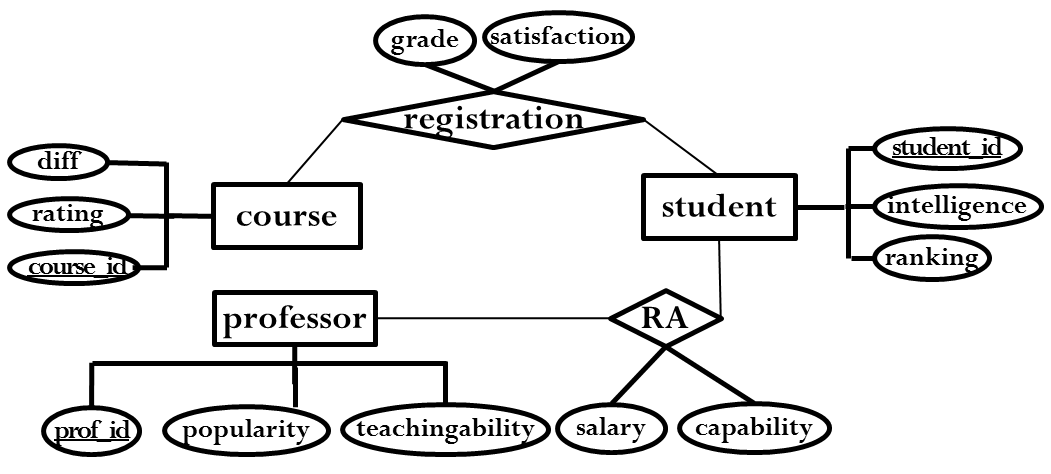
\includegraphics[width=0.5\textwidth]{figures/university-schema.png} 
%} 
%\caption{A relational ER Design for a university domain.}
% \label{fig:university-schema}
%\end{figure}
%
% We begin with a standard \textbf{relational schema} containing a set of tables, each with key fields, %typically
%descriptive attributes, and possibly foreign key pointers. 
%A \textbf{database instance} specifies the tuples contained in the tables of a given database schema. 
%We assume that tables in the relational schema can be divided into {\em entity tables} and {\em relationship tables.} 
%This is the case whenever a relational schema is derived from an entity-relationship model (ER model) \cite[Ch.2.2]{Ullman1982}. 
%The functor formalism is rich enough to represent the constraints of an ER schema by the following translation: Entity sets correspond to types, descriptive attributes to functions, relationship tables to predicates, and foreign key constraints to type constraints on the arguments of relationship predicates.  
%Assuming an ER design, a relational structure can be visualized as a complex network \cite[Ch.8.2.1]{Russell2010}: individuals are nodes, attributes of individuals are node labels, relationships correspond to (hyper)edges, and attributes of relationships are edge labels. Conversely, a complex  network can be represented using a relational database schema.


%Table \ref{table:university-schema} shows a relational schema for a database related to a university.
%In this example, there are three entity tables: a $\student$ table, a $\course$ table and a $\prof$ table.  
%The relationship table $\reg$ with foreign key pointers to the $\student$ and $\course$ tables whose tuples indicate which students have registered in which courses.
%
%The other two relationship tables have the similar foreign key constraints involving different entity tables. 
%
%Figure \ref{fig:university-tables} displays a small database instance for this schema together with a Parametrized Bayes Net (only considering the $\reg$ relationship for simplicity.) 
%%To keep the schema simple, we introduce only a limited number of attributes for each entity class. 
%
% 
%\begin{figure}[htbp] %  figure placement: here, top, bottom, or page
% \centering
%\resizebox{0.5\textwidth}{!}{
% 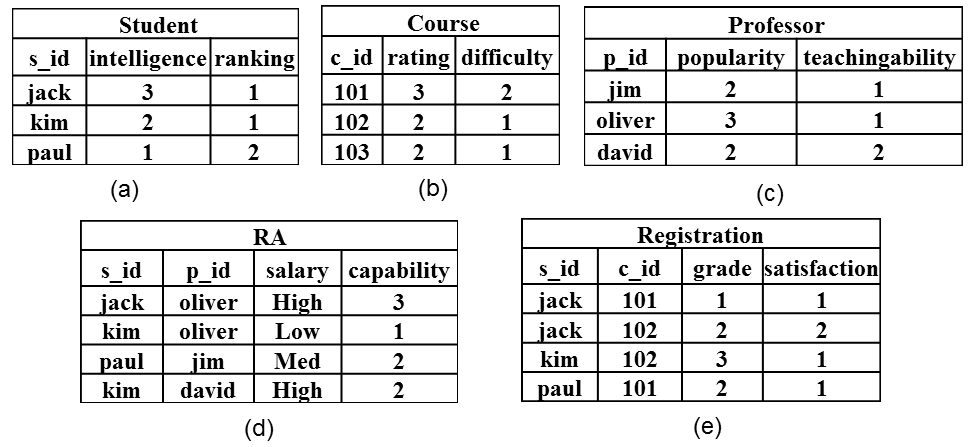
\includegraphics[width=0.5\textwidth]{figures/university-tables.png} 
%} 
%\caption{Database Table Instances: (a) $\student$, (b) $\course$, (c) $\reg$.  (d)A sample Parametrized Bayes Net based on the university schema.  % The $\cttable(\reg)$ table  is the contingency table for $\reg$ which we will introduce in Section~\ref {sec:mobius}. (e) 
%}
% \label{fig:university-tables}
%\end{figure}
%


%\subsection{Propositional Machine Learning}
%bla,bla,

%\subsection{Bayes Nets for Relational Data}
%Poole introduced the Parametrized Bayes net (PBN) formalism that combines Bayes nets with logical syntax for expressing relational concepts \cite{Poole2003}. We adopt the PBN formalism, following Poole's presentation.
%A \textbf{population} is a set of individuals.
%Individuals are denoted by lower case expressions (e.g., $\it{bob}$). 
%%A \textbf{population variable} is capitalized. 
%A \textbf{functor} represents a mapping
%$\functor: \population_{1},\ldots,\population_{a} \rightarrow \outdomain_{\functor}$
%where $\functor$ is the name of the functor, each $\population_{i}$ is a population, and $\outdomain_{\functor}$ is the output type or \textbf{range} of the functor. 
%In this paper we consider only functors with a finite range, disjoint from all populations.  If $\outdomain_{\functor} = \{\true,\false\}$, the functor $\functor$ is a (Boolean) \textbf{predicate}. A predicate with more than one argument is called a \textbf{relationship}; other functors are called \textbf{attributes}. We use uppercase for predicates and lowercase for other functors.
%
%
%
%%the populations associated with 
% %the variables are of the appropriate type for the functor.
%%A \textbf{Parametrized random variable} (PRV) is of the form $\functor(\X_{1},\ldots,\X_{a})$, where each $\X_{i}$ is a 1st-order variable. 
%Each 1st-order variable is associated with a population that specifies its domain or type. 
%We refer to the 1st-order variables as population variables to distinguish them from the parametrized random variables. %that appear in a Bayes net model. 
%
%
%Figure \ref{fig:university-tables} displays a small database instance for this schema together with a Parametrized Bayes Net (only considering the $\ra$ relationship for simplicity.) 
%%To keep the schema simple, we introduce only a limited number of attributes for each entity class. 
%
% 
%\begin{figure}[htbp] %  figure placement: here, top, bottom, or page
% \centering
%\resizebox{0.4\textwidth}{!}{
% 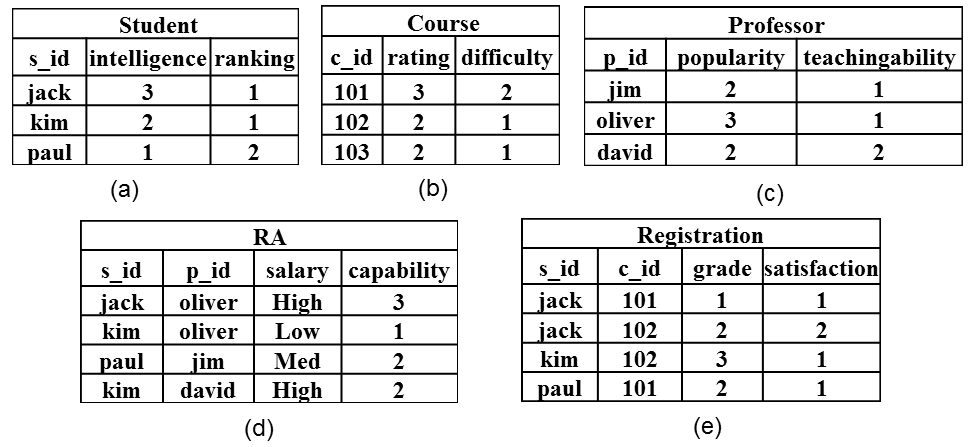
\includegraphics[width=0.5\textwidth]{figures/university-tables.png} 
%} 
%\caption{Database Table Instances: (a) $\student$, (b) $\prof$, (c) $\ra$.  (d) A sample Parametrized Bayes Net based on the university schema.  % The $\cttable(\reg)$ table  is the contingency table for $\reg$ which we will introduce in Section~\ref {sec:mobius}. (e) 
%}
% \label{fig:university-tables}
%\end{figure}




\section{The Random Variable Database} 

Statistical analysis is based on a set of random variables. Formally, a random variable $\node$ is defined by a domain of possible values and a probability distribution over that domain. In this section we discuss what types of random variables are suitable for analyzing relational databases; we refer to these as {\em relational random variables.} We also discuss how to find and store relevant metainformation about relational random variables. The metainformation for a random variable must include the following at a minimum.

\begin{enumerate}
\item The domain of the random variable. For instance, a range of continuous values, or a finite set of discrete values.
\item Pointers to the table and/or column in the original database that contains the data relevant to the random variables. 
\end{enumerate}

There are various different notational systems for defining random variables in relational structures, of equivalent expressive power. We adopt function-based notation from logic for combining statistical and relational concepts \cite{Russell2010}. As we discuss below, the expressive power of this formalism is equivalent to well-known logical query languages such as the domain relational calculus. Our approach can be easily adapted for other notational systems.

\subsection{Relational Random Variables}
A domain or \textbf{population} is a set of individuals.
Individuals are denoted by lower case expressions (e.g., $\it{bob}$). 
%A \textbf{first-order variable} is capitalized. 
A \textbf{functor} represents a mapping
$\functor: \population_{1},\ldots,\population_{a} \rightarrow \outdomain_{\functor}$
where $\functor$ is the name of the functor, each $\population_{i}$ is a population, and $\outdomain_{\functor}$ is the output type or \textbf{range} of the functor. 
In this paper we consider only functors with a finite range, disjoint from all populations.  If $\outdomain_{\functor} = \{\true,\false\}$, the functor $\functor$ is a (Boolean) \textbf{predicate}. A predicate with more than one argument is called a \textbf{relationship}; other functors are called \textbf{attributes}. We use uppercase for predicates and lowercase for other functors. Throughout this paper we assume that all relationships are binary, though this is not essential for our algorithm.
%the populations associated with 
 %the variables are of the appropriate type for the functor.
%
A \textbf{Relational random variable} (RRV) is of the form $\functor(\X_{1},\ldots,\X_{a})$, where each $\X_{i}$ is a first-order variable \cite{Poole2003}. 
Each first-order variable is associated with a population/type. In the context of RRVs, we therefore refer to first-order variables also as \textbf{population variables}. An RRV has two components: A functor and a list of population variables. We discuss first how to translate a relational database schema into a set of functors. Second, we describe a default method for combining population variables with functors. 

\textbf{mention Schema Analyzer that gives me the variables}

\subsection{Translating Entity-Relationship Models Into Functors}
 We begin with a standard \textbf{relational schema} containing a set of tables, each with key fields, %typically
descriptive attributes, and possibly foreign key pointers. 
A \textbf{database instance} specifies the tuples contained in the tables of a given database schema. 
We assume that tables in the relational schema can be divided into {\em entity tables} and {\em relationship tables.} 
This is the case whenever a relational schema is derived from an entity-relationship model (ER model) \cite[Ch.2.2]{Ullman1982}. Figure~\ref{fig:university-schema} shows an ER diagram for a toy university domain. An ER diagram shows entity sets as boxes, relationships between entities as diamonds, and attributes as ovals. Our approach is to translate the components of the ER diagram into random variables for statistical analysis \cite{Heckerman+al:SRL07}. Figure~\ref{fig:instance} shows a database instance for this ER diagram.


\begin{figure}[htbp] %  figure placement: here, top, bottom, or page
 \centering
\resizebox{0.4\textwidth}{!}{
 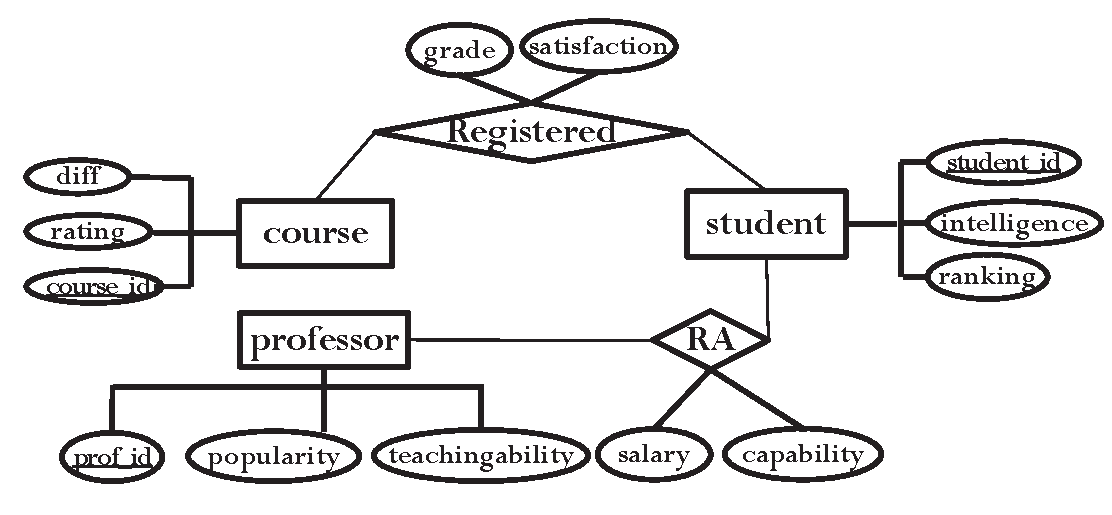
\includegraphics[width=0.5\textwidth]{university-schema.pdf} 
} 
\caption{A relational ER Design for a university domain.}
 \label{fig:university-schema}
\end{figure}


\begin{figure}[htbp] %  figure placement: here, top, bottom, or page
 \centering
\resizebox{0.4\textwidth}{!}{
 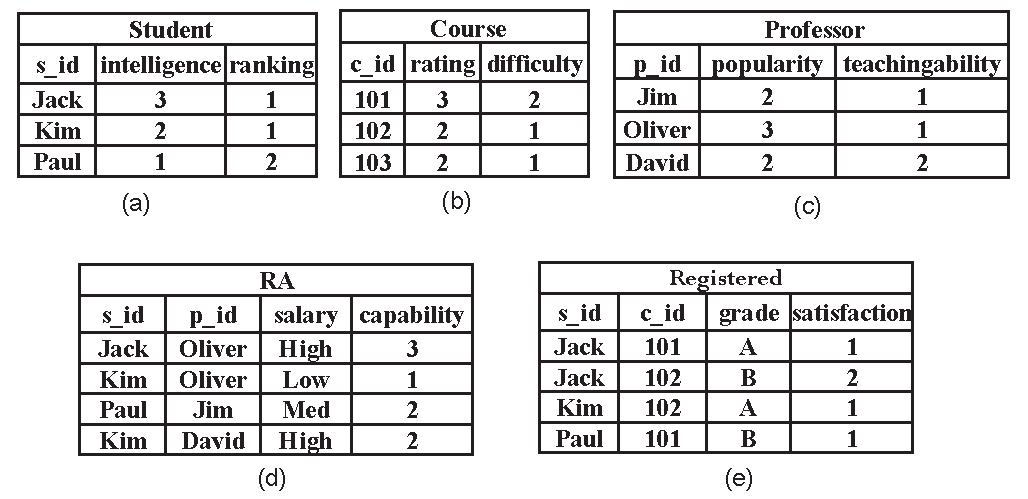
\includegraphics[width=0.5\textwidth]{university-tables.pdf} 
} 
\caption{Database Table Instances: (a) $\student$, (b) $\course$, (c) $\prof$, (d) $\ra$, (e) $\reg$.  
}
 \label{fig:instance}
\end{figure}


The functor formalism is rich enough to represent the constraints of an entity-relationship schema via the following translation: Entity sets correspond to populations, descriptive attributes to attribute functors, relationship tables to relationship functors, and foreign key constraints to type constraints on the arguments of relationship predicates. The translation of an ER diagram into a set of functors converts each element of the diagram into a functor, except for entity sets and key fields. Table~\ref{table:translation} illustrates this translation.
%, distinguishing attributes of entities ($\eatts$) and attributes of relationships ($\ratts$). 


%\begin{table}[btp] \centering
%\resizebox{0.4\textwidth}{!}{
%\begin{tabular}[c]
%{|l|c|l|l|}\hline
% ER Design &Type & Functor &\RRV \\\hline
%    \begin{tabular}{l}Entity \\Tables\end{tabular}&\begin{tabular}{l}Population \\Variables \end{tabular} & Student, Course & S, C \\\hline
%    \begin{tabular}{l}Relation \\Tables \end{tabular}&RNodes &RA & RA(P,S) \\\hline
%   \begin{tabular}{l}Entity \\Attributes \end{tabular}&1Nodes & intelligence, ranking &\begin{tabular}{l} \{intelligence(S), ranking(S)\}  \\=1Nodes(S) \end{tabular} \\\hline
%  \begin{tabular}{l} Relationship \\Attributes \end{tabular}&2Nodes & teachingability, salary &\begin{tabular}{l}   \{teachingability(P,S), salary(P,S)\}  \\= 2Nodes(RA(P,S))\end{tabular}\\\hline
%   
%\end{tabular}
%}
% % end scalebox
%\caption{Translation from ER Diagram to Relational Random Variable. \textbf{OS fix table}
% \label{table:translation}}
%\end{table}
\begin{table}[btp] \centering
\resizebox{0.4\textwidth}{!}{
\begin{tabular}[c]
{|l|c|l|l|}\hline
 ER Design &Type & Functor &\RRV \\\hline
    \begin{tabular}{l}Entity \\Tables\end{tabular}&\begin{tabular}{l}Population \\Variables \end{tabular} & Student, Course & $\S, \C$ \\\hline
    \begin{tabular}{l}Relation \\Tables \end{tabular}&Relationship &RA & RA($\P$,$\S$) \\\hline
   \begin{tabular}{l}Entity \\Attributes \end{tabular}&1Attributes & intelligence, ranking &\begin{tabular}{l} \{intelligence($\S$), ranking($\S$)\}  \\=1Attributes($\S$) \end{tabular} \\\hline
  \begin{tabular}{l} Relationship \\Attributes \end{tabular}&2Attributes & capability, salary &\begin{tabular}{l}   \{capability($\P, \S$), salary($\P, \S$)\}  \\= 2Attributes(RA($\P, \S$))\end{tabular}\\\hline
   
\end{tabular}
}
 % end scalebox
\caption{Translation from ER Diagram to Relational Random Variable. %\textbf{OS fix table}
 \label{table:translation}}
\end{table}



There are different types of functors corresponding to the different types of ER diagram components. From a statistical point of view, the simplest type represents an attribute of an entity set. We refer to such functors as \textbf{1Attributes}. In Figure~\ref{fig:university-schema}, there are six 1Attributes corresponding to attributes of Professors (2), Students (2), and Courses (2). 
%The primary keys (p\_id, s\_id, c\_id) are identifiers that are not treated as random variables. 
The metainformation about 1Attributes can be stored in a database table as shown in Figure~\ref{fig:attributes}. 

\begin{figure}[htbp] %  figure placement: here, top, bottom, or page
 \centering
\resizebox{0.4\textwidth}{!}{
 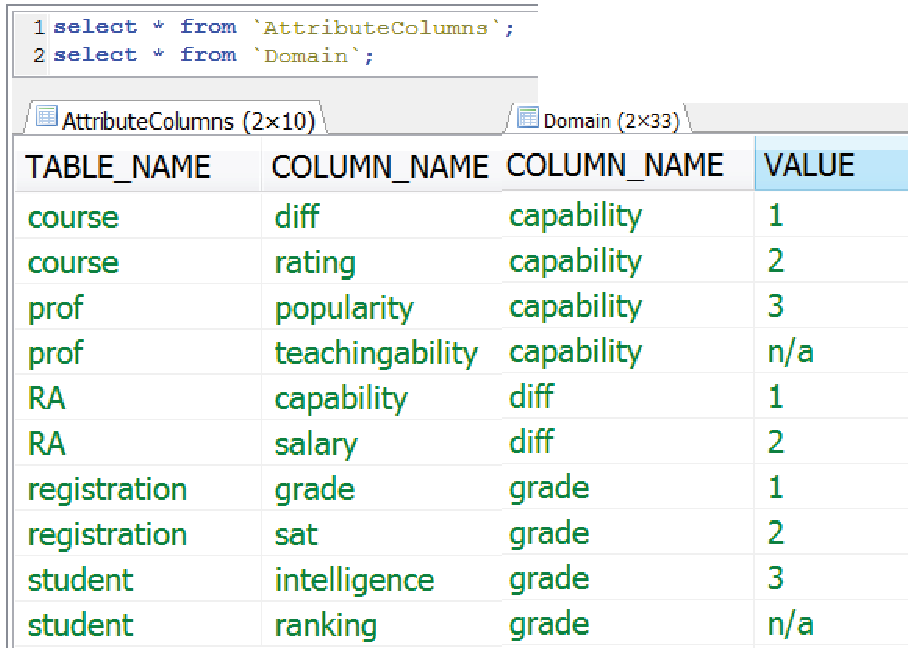
\includegraphics[width=0.5\textwidth]{attribute-domain.pdf} 
} 
\caption{The metainformation about attributes represented in database tables.  
}
 \label{fig:attributes}
\end{figure}

1Attributes correspond to {\em columns}, just as random variables in single-table data do. Relationship functors have the Boolean domain $\{\true,\false\}$. Relationship functors correspond to {\em tables}, not columns. There are two relationship variables in the diagram~\ref{fig:university-schema} corresponding to the $\it{Registered}$ and $\it{RA}$ relationships. A relationship table stores the information about which entities are related to each other in a certain way. For example, the database instance of Figure~\ref{fig:instance} represents that student Jack took course 101, and that student Kim did not take course 101. Including a relationship random variable in a statistical model allows the model to represent uncertainty about whether or not a relationship exists \cite{linkGetoor2003,domingos}. This supports applications like link prediction, (e.g., predicting whether two users are friends, \cite{Liben-Nowell2007}), and multiple link analysis for finding correlations among relationships (e.g., if user $u$ performs a web search for item $i$, is it likely that $u$ watches a video about $i$ ?). 
%
%Managing relationships raises several new issues compared to managing single-table column-based variables. 
To relate a relationship variable to the original relationship data, we need to store pointers to the related entity sets as metainformation. 

We refer to attributes of relationships as \textbf{2Attributes}. In Figure~\ref{fig:university-schema}, there are four 2Attributes corresponding to attributes of Registered (2) and RA (2). An important issue for relational data is that the values of descriptive attributes of relationships are undefined for entities that are not related. Following \cite{Russell2010}, we represent this by introducing a new constant $\it{n/a}$ in the domain of a 2Variable; see Figure~\ref{fig:attributes}.
%\cite{BLOG}, 
%$\it{capability(\P,\S)} = n/a $
%we indicate this by writing 
%%$\it{grade}(\s,\c) = n/a$ 
%$\it{capability(\P,\S)} = n/a $ for a reserved constant $\it{n/a}$. 
%The assertion $\it{capability(\P,\S)}$ = n/a is therefore equivalent to the assertion that $\ra(\P,\S) = \false$.

%\subsection{Generating Default Relational Random Variables}

%We use upper case for Boolean-valued variables with domain $\{\true,\false\}$, such as RVariables. We use
%lower case for other random variables. 

\subsection{Population Variables and Self-Relationships}

Next we discuss how to combine population variables with functors to obtain full RRVs. The random variable database specifies a set of population variables. With each population variable, we store a pointer to the original entity table as metainformation. For example, the $\it{S}$ population variable is associated with the the $\it{Student}$ table in the original database. 
In the example of Figure~\ref{fig:university-schema}, the type/foreign key constraints on the functors determine which population variables to add, as shown in Table~\ref{table:translation}. In this case adding population variables to functors enhances readability but is redundant given the type information. 

The additional expressive power from population variables becomes important in the presence of self-relationships \cite{Heckerman+al:SRL07}. 
A self-relationship relates two entities of the same type.
%, when we need to introduce more than one relationship node for the relationship functor. 
For example, the Mondial database contains a self-relationship $\it{Borders}$ that relates two countries, as shown in the ER diagram Figure~\ref{fig:mondial-er}. Neville and Jensen provide evidence that self-relationships are very common, so it is important to accommodate them in a statistical model \cite{Neville2007}. Self-relationships give rise to relational autocorrelations, where the attribute value of an entity depends probabilistically on the attribute value of related entities \cite{Neville2007}. 
Relational autocorrelations are analogous to temporal autocorrelations in time series analysis, where there is a correlation between the value of a quantity at one time and the value of the same quantity at another. An autocorrelation cannot be represented in a model that contains only one random variable referring to the quantity in question. For time series, a common solution is to introduce {\em two} distinct random variables  that refer to the same quantity, but at different times. For instance, we may have two random variables $\it{temperature}_{t}$ and $\it{temperature}_{t+1}$. Similarly, to represent a relational autocorrelation between the continents of two different countries, we may introduce two random variables $\it{continent}_{\C_{1}}$ and $\it{continent}_{\C_{2}}$. The index notation can equivalently be replaced by function notation, where we write $\it{continent}(\C_{1})$ and $\it{continent}(\C_{2})$ \cite{Milch2007}. This leads to the concept of a relational random variable as previously defined. 

%In the ER diagram, there are two lines from the $\it{Countries}$ entity set to the $\it{Borders}$ relationship set 
%The ring structure may be represented with two different population variables that each refer to the $\it{Countries}$ entity set. 
The corresponding relationship random variable is $\it{Borders}(\C_{1},\C_{2})$. The different positions of the 1st-order variables can represent different roles in the relationship. A random variable for a descriptive 2Attribute can also be represented using population variables, for instance $\it{Border\_Length}(\C_{1},\C_{2})$. %\textbf{OS: add ER diagram for this simple Mondial example}. 
This notation is expressive enough to represent autocorrelations. 
For instance, the association rule
$$\it{continent}(\C_{1}) = \it{Europe}, \it{Borders}(\C_{1}, \C_{2}) = \true \rightarrow \it{continent}(\C_{2}) = \it{Europe}$$
Some complex patterns require more than one relationship variable for the same relationship functor. For instance, representing transitivity requires three relationship variables as in 
$$\it{Borders}(\C_{1}, \C_{2}) = \true,  \it{Borders}(\C_{1}, \C_{3}) = \true \rightarrow \it{Borders}(\C_{1}, \C_{3}) = \true.$$
expresses that if two countries are neighbors and one is in Europe, the other country is likely to be in Europe. By default, our system creates three such copies for every self-relationship, together with the applicable 1Variables (e.g., $\it{continent}(\C_{3}$).
%Since we introduce two population variables referring to the same entity set, we need to duplicate the 1Nodes for that entity set. 
%This allows the logical language to represent that attributes of neighboring countries influence each other, 
%%Using a second relationship node with the $\it{Borders}$ functor allows us to represent such influences, 
%for instance in the following rule
%$$\it{continent}(\C_{1}) = \it{Europe}, \it{Borders}(\C_{1}, \C_{2}) = \true \rightarrow \it{continent}(\C_{2}).$$
If the database schema contains a self-relationship, our script adds one population variable for each role in the relationship in the default database. For each population variable there is a separate set of corresponding 1Nodes. In the Mondial example, there are two 1Nodes $\it{continent}(\C_{1})$ and $\it{continent}(\C_{2})$.
\begin{figure}[htbp] %  figure placement: here, top, bottom, or page
 \centering
\resizebox{0.4\textwidth}{!}{
 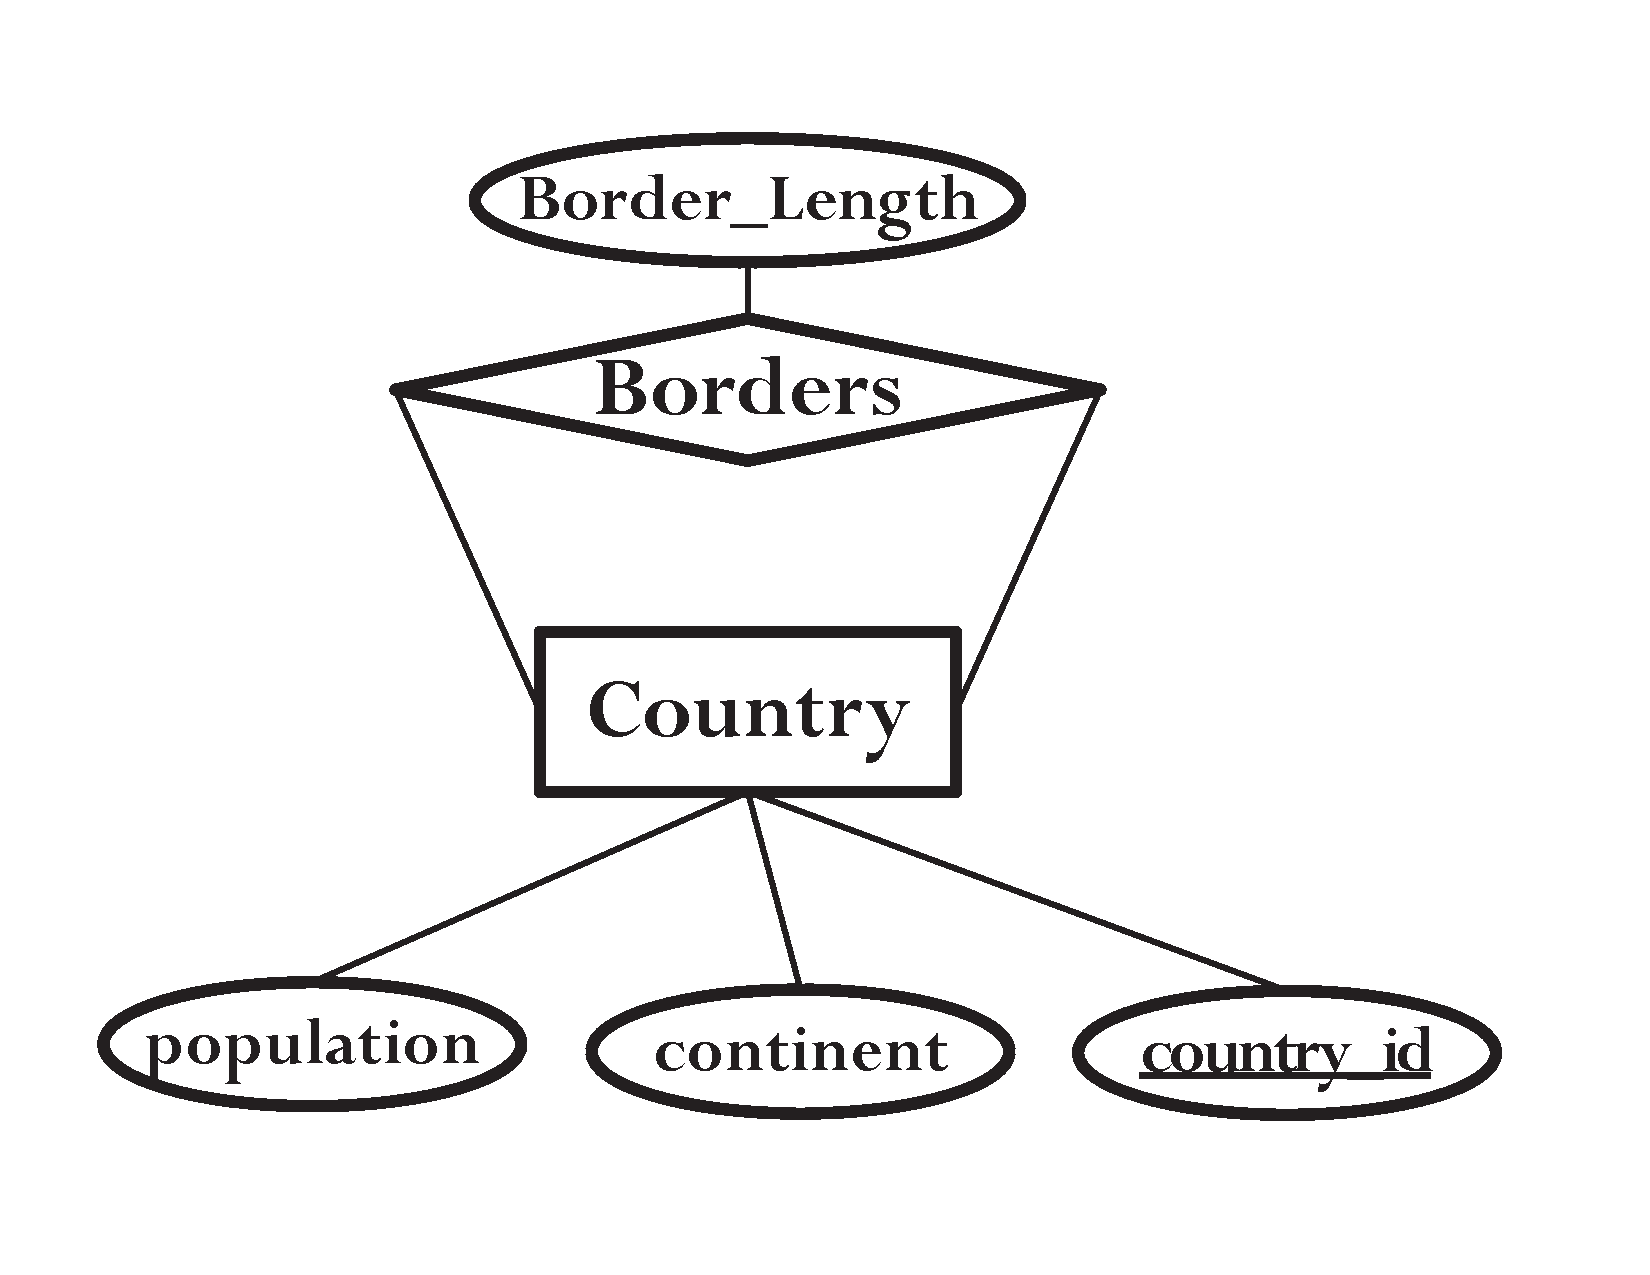
\includegraphics[width=0.5\textwidth]{mondial-er.pdf} 
} 
\caption{The ER diagram for Mondial database. $\it{Borders}$ is a self-relationship. 
}
 \label{fig:mondial-er}
\end{figure}

%\textbf{OS: make table for random variable database}
%move  to the appendix
%\begin{table}[htbp]
%  \centering
%\resizebox{0.5\textwidth}{!}{
%    \begin{tabular}{|r|r|r|r|r|r|}
%    \hline
%    \multicolumn{2}{|c|}{Table Name} & \multicolumn{4}{c|}{Schema}  \\
%    \hline
%    \multicolumn{2}{|l|}{AttributeColumns} & \multicolumn{4}{l|}{\begin{tabular}{l}TABLE\_NAME,  COLUMN\_NAME   \end{tabular}}  \\
%    \hline
%    \multicolumn{2}{|l|}{Domain} & \multicolumn{4}{l|}{\begin{tabular}{l}COLUMN\_NAME, VALUE   \end{tabular}}  \\
%    \hline
%    \multicolumn{2}{|l|}{Pvariables} & \multicolumn{4}{l|}{\begin{tabular}{l}Pvid,  TABLE\_NAME  \end{tabular}}  \\
%    \hline
%    \multicolumn{2}{|l|}{1Variables} & \multicolumn{4}{l|}{\begin{tabular}{l}1VarID,  COLUMN\_NAME,  Pvid 
%\end{tabular} }  \\
%    \hline
%    \multicolumn{2}{|l|}{2Variables } & \multicolumn{4}{l|}{\begin{tabular}{ll} 2VarID,  COLUMN\_NAME,  Pvid1,  Pvid2, \\ TABLE\_NAME \end{tabular}}  \\
%    \hline
%    \multicolumn{2}{|l|}{Relationship} & \multicolumn{4}{l|}{\begin{tabular}{lll}RVarID,  TABLE\_NAME, Pvid1,  Pvid2, \\ COLUMN\_NAME1,  COLUMN\_NAME2  \end{tabular}}  \\
%    \hline
%    \end{tabular}%
%}
%  \caption{Schema for Random Variable Database}
%  \label{table:rvdb}%
%\end{table}%




%To build a table with definitions of nodes, we represent a node as a tuple of the form $\langle \functor, \it{pv}_1, \ldots, \it{pv}_\ell \rangle$; in this paper we assume that  $\ell = 1,2$. Table~\ref{table:translation} shows examples.
%Adding population variables to functors generally requires only utilizing the primary key information to find which entities are associated with each functor and then using the population variables constructed in the previous step. If we find a self-relationship, we add one population variable for each role in the relationship, and one set of 1Nodes for each population variable. 

\subsection{SQL Implementation}

The metainformation about the random variables is stored in the \textbf{random variable database} (RVDB). The relational schema of the RVDB is shown in Figure~\ref{fig:rv_db}. %\textbf{OS: make 6 relations}. 
The relational schema of the original database is represented in tables in the database system catalog. Given that both the system catalog and the RVDB are databases, we can use SQL to transfer information from one to the other. %\textbf{OS make SQL query} 
We show an SQL query for extracting the metainformation about 1Attributes from the system catalog. The exact name and format of this catalog is system-dependent; our query works for MySQL version 5.5. The remaining components of our model manager depend only on the metainformation in the RVDB, not on the system catalog.
Our second SQL query shows the construction of RVariables in our university example. This illustrates the use of foreign key information from the system catalog. The full SQL script also constructs tables for 2Attributes, recognizes self-relationships by using foreign key pointer information, and constructs relationship variables for the same relationship when necessary. The full script is included in the supplementary material. 

After the random variable database has been created from the system catalog, the user  can add or substract relational random variables depending on the statistical patterns of interest.
\begin{alltt}
CREATE TABLE  KeyColumns AS SELECT * FROM
(SELECT TABLE_NAME, COLUMN_NAME, CONSTRAINT_NAME 
FROM  INFORMATION_SCHEMA.KEY_COLUMN_USAGE
WHERE  (KEY_COLUMN_USAGE.TABLE_SCHEMA = 'uni'))
 as A NATURAL JOIN 
(SELECT COLUMNS.TABLE_NAME, COLUMNS.COLUMN_NAME     
FROM   INFORMATION_SCHEMA.COLUMNS,    
INFORMATION_SCHEMA.TABLES
WHERE  (COLUMNS.TABLE_SCHEMA = `uni'        
AND TABLES.TABLE_SCHEMA = `uni'
AND TABLES.TABLE_NAME = COLUMNS.TABLE_NAME 
AND TABLES.TABLE_TYPE = `BASE TABLE') ) as B;

CREATE TABLE PVariables AS  SELECT 
CONCAT(EntityTables.TABLE_NAME, `0') AS pvid,
EntityTables.TABLE_NAME FROM
(SELECT distinct TABLE_NAME, COLUMN_NAME 
FROM   KeyColumns T WHERE
1 = (SELECT  COUNT(COLUMN_NAME)   
FROM   KeyColumns T2  WHERE     
T.TABLE_NAME = T2.TABLE_NAME
AND CONSTRAINT_NAME = 'PRIMARY')) 
as EntityTables 

CREATE TABLE 1Variables AS
SELECT CONCAT(`\`', COLUMN_NAME,
 `(', pvid, `)', `\`') AS 1VarID,
COLUMN_NAME,   pvid  FROM    
PVariables   NATURAL JOIN  AttributeColumns;

\end{alltt}

%\begin{quote}
%CREATE TABLE 1VARIABLES AS SELECT \\
%CONCAT($'`'$, COLUMN\_NAME, $'(', $pvid,$ ')', '`')$ AS 1VarID,\\
%COLUMN\_NAME,    pvid\\
%%    index\_number = 0 AS main \\
%FROM\\
%PVariables        NATURAL JOIN    AttributeColumns;
%\end{quote}
%\subsection{The Random Variable Database}
%The information about the random variables is stored in the \textbf{random variable database}.  
%%This database provides metainformation for machine learning analysis analogous to the way in which the system catalog provides metainformation for database queries. The definitions of the random variables are stored in tables in the random variable database, together with useful metainformation about the random variables, such as their domains and the sizes of their domains. 
%%
%The Virtual Join algorithm distinguishes three types of PRVs, 1Nodes, RNodes, and 2Nodes. 
%For each attribute of an entity, there is a corresponding attribute node called a \textbf{1Node} for short. The domain of a 1Node is the same as that of the corresponding attribute.  There is a Boolean random variable for each relationship set, called a \textbf{relationship node} or \textbf{RNode} for short.
%Throughout this paper we assume that all relationships are binary, though this is not essential for our algorithm. 
%For each attribute of an relationship, there is a corresponding attribute node called a \textbf{2Node} for short. The domain of a 2Node is the same as that of the corresponding attribute. 
%%In logical terms, nodes are interpreted as functions that return a value for a given input entity tuple \cite{Milch2007}.
%Table~\ref{table:translation} illustrates %the mapping from the ER design to 
%the logical functor notation and its relationship to the database ER diagram. 

%
%The basic set of random variables is derived from the elements of an ER design.
%Table~\ref{table:translation} illustrates the mapping from the ER design to the logical functor notation. 
%There is a random variable for each entity set, called a \textbf{population variable}. 
%The domain of population variables comprises the entities in the associated entity set. 
%There is a Boolean random variable for each relationship set, called a \textbf{relationship node} or \textbf{RNode} for short.
%Throughout this paper we assume that all relationships are binary, though this is not essential for our system. 
%For each attribute of an entity, there is a corresponding attribute node called a \textbf{1Node} for short. The domain of a 1Node is the same as that of the corresponding attribute.  
%For each attribute of an relationship, there is a corresponding attribute node called a \textbf{2Node} for short. The domain of a 2Node is the same as that of the corresponding attribute. 
%In logical terms, nodes are interpreted as functions that return a value for a given input entity tuple \cite{Milch2007}.
%As the table shows, we refer to the attributes of a population variable $\A$ collectively as $1Nodes(\A)$ and to the attributes of a relationship node $\R$ collectively as $2Nodes(\R)$. %\cite{BLOG}. 

%The value of a relationship attribute is undefined for entities that are not related.
% For example, if student $\s$ is not registered in course $\c$, the value of $\it{grade}(\s,\c)$ is undefined. 
%Following \cite{Milch2007}, 
%%\cite{BLOG}, 
%we indicate this by writing $\it{grade}(\s,\c) = n/a$ for a reserved constant $\it{n/a}$. 
%The assertion $\it{grade}(\s,\c) = n/a$ is therefore equivalent to the assertion that $\reg(\s,\c) = \false$.
 



%\begin{figure}[htbp]
%\begin{center}
%\resizebox{0.5\textwidth}{!}{
%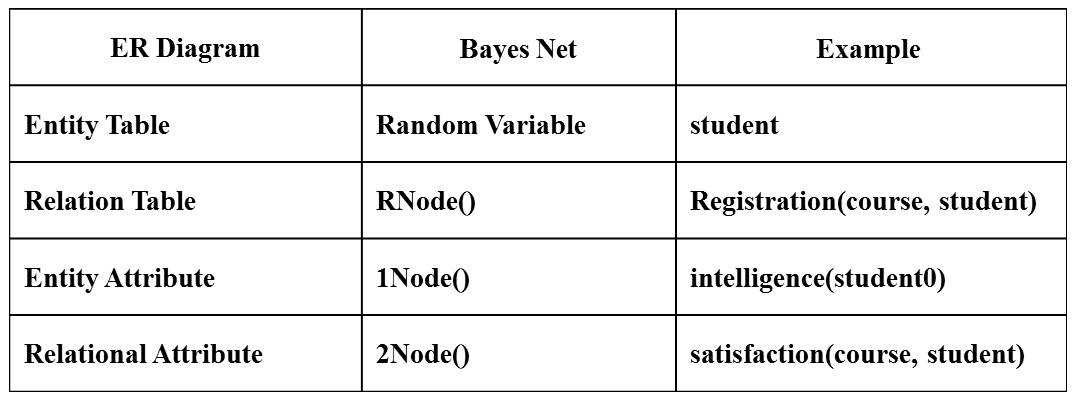
\includegraphics[width=0.5\textwidth]{figures/translation.png}
%}
%\caption{Translation from ER Diagram of Relational Database to Bayes Nets.
%\label{fig:translation}}
%\end{center}
%\end{figure}

%\begin{table}[btp] \centering
%\resizebox{0.5\textwidth}{!}{
%\begin{tabular}[c]
%{|l|l|l|l|}\hline
% ER Design &Bayes Net & Example &Term Notation\\\hline
%    Entity Tables&Population Variables  & Student, Course & S, C \\\hline
%    Relation Tables &RNodes &Registered & Registered(C,S) \\\hline
%   Entity Attributes &1Nodes & intelligence, ranking & \{intelligence(S), ranking(S)\} = 1Nodes(S) \\\hline
%   Relationship Attributes &2Nodes & satisfaction, grade & \{satisfaction(C, S), grade(C,S)\} = 2Nodes(Registered(C,S)) \\\hline
%   
%\end{tabular}
%}
% % end scalebox
%\caption{Translation from ER Design of Relational Database to Bayes Nets.
% \label{table:translation}}
%\end{table}
%\begin{table}[btp] \centering
%\resizebox{0.4\textwidth}{!}{
%\begin{tabular}[c]
%{|l|c|l|l|}\hline
% ER Design &Type & Functor &PRV \\\hline
%   % \begin{tabular}{l}Entity \\Tables\end{tabular}&\begin{tabular}{l}Population \\Variables \end{tabular} & Student, Course & S, C \\\hline
%    \begin{tabular}{l}Relation \\Tables \end{tabular}&RNodes &RA & RA(P,S) \\\hline
%   \begin{tabular}{l}Entity \\Attributes \end{tabular}&1Nodes & intelligence, ranking &\begin{tabular}{l} \{intelligence(S), ranking(S)\}  \\=1Nodes(S) \end{tabular} \\\hline
%  \begin{tabular}{l} Relationship \\Attributes \end{tabular}&2Nodes & teachingability, salary &\begin{tabular}{l}   \{teachingability(P,S), salary(P,S)\}  \\= 2Nodes(RA(P,S))\end{tabular}\\\hline
%   
%\end{tabular}
%}
% % end scalebox
%\caption{Translation from ER Diagram to Relational Random Variables.
% \label{table:translation}}
%\end{table}

%{\em Database Representation.} 
%The definitions of the three types of PRVs are listed in three tables in the
% Random Variable Database. 
%This database also provides information about the random variables that is required for learning, such as their domains and the sizes of their domains. We refer to this as \textbf{metainformation}. Utilizing the metainformation allows us to develop general schema-independent learning algorithms. 
%
%\subsection{Generating Default PRVs} Defining a set of PRVs for a given database requires some user expertise in translating domain knowledge into the functor representation and metainformation.
%% terms of understanding the functor representation and extracting metainformation. 
%An alternative is to exploit the database schema catalog to generate default random variable database.
%We use this default in the experiments reported below.  
%Given an ER-diagram, it is straightforward to generate functors as illustrated in Table~\ref{table:translation}.
% Given a database information schema, we can compute an implicit ER diagram by reversing the standard translation from ER-diagrams to SQL \cite{Ullman1982}.
%For instance, if a table contains a single primary key column and no foreign key pointers, we treat it as representing an entity set and associate a population variable with it. 
%Since the database information schema is itself stored in table form, the default random variable database can be created using an SQL script. 
%We omit further details due to space constraints.
%
%The main complication arises when the database contains a self-relationship \cite{Heckermann} that relates two entities of the same type.
%%, when we need to introduce more than one relationship node for the relationship functor. 
%For example, the Mondial database contains a self-relationship $\it{Borders}$ that relates two countries. 
%%In the ER diagram, there are two lines from the $\it{Countries}$ entity set to the $\it{Borders}$ relationship set 
%%The ring structure may be represented with two different population variables that each refer to the $\it{Countries}$ entity set. 
%The corresponding relationship node is $\it{Borders}(\C_{1},\C_{2})$ . The different positions of the 1st-order variables can represent different roles in the relationship. 
%%Since we introduce two population variables referring to the same entity set, we need to duplicate the 1Nodes for that entity set. 
%%This allows the logical language to represent that attributes of neighboring countries influence each other, 
%%%Using a second relationship node with the $\it{Borders}$ functor allows us to represent such influences, 
%%for instance in the following rule
%%$$\it{continent}(\C_{1}) = \it{Europe}, \it{Borders}(\C_{1}, \C_{2}) = \true \rightarrow \it{continent}(\C_{2}).$$
%If the database schema contains a self-relationship, our script adds one population variable for each role in the relationship in the default database. For each population variable there is a separate set of corresponding 1Nodes. In the Mondial example, there are two 1Nodes $\it{continent}(\C_{1})$ and $\it{continent}(\C_{2})$.
%
%
%To build a table with definitions of nodes, we represent a node as a tuple of the form $\langle \functor, \it{pv}_1, \ldots, \it{pv}_\ell \rangle$; in this paper we assume that  $\ell = 1,2$. Table~\ref{table:translation} shows examples.
%Adding population variables to functors generally requires only utilizing the primary key information to find which entities are associated with each functor and then using the population variables constructed in the previous step. If we find a self-relationship, we add one population variable for each role in the relationship, and one set of 1Nodes for each population variable. 
%
%We first discuss computing a default set of population variables and functors from the schema information, then combining the variables with the functors to form terms.
%
%\begin{algorithm}[htbp]
%\caption{Generating a default set of functors for modelling a target database. Can be implemented with SQL queries to the database information schema.}
%\label{alg:functors}
%%\linesnumbered
%\SetKwData{KwCalls}{Calls}
%\SetKwData{KwCondition}{Precondition:}
%\KwIn{Database Information Schema; Target Database $\D$}
%\KwOut{Tables with meta information about functors, stored in the random variable database $\D_{\RV}$.}
%\begin{algorithmic}[1]
%\STATE Find tables in $\D$ with a single primary key field. Store table names in $\D_{\RV}.\it{EntityTables}$.
%\STATE For each entity table, %.
%add one population variable entry $(\it{pv})$ in $\D_{\RV}.\it{Pvariables}$.
%\STATE For each entity table, for each column that is not part of the primary key, add an entry $(\it{column\_name})$ in $\D_{\RV}.\it{1Functors}$.
%%\STATE For each entity table, for each column that is not part of the primary key, add an entry $(\it{column\_name},\it{pv})$ in $\D_{\RV}.\it{1Functors}$.
%\STATE Find tables in $\D$ with two primary key columns that reference entity tables. Store table names in $\D_{\RV}.\it{RelationTables}$.
%% \STATE For each relation table, add an entry $(\it{table\_name}, \it{pv}_{1}, \it{pv}_{2})$ to $\D_{\RV}.
% \STATE For each relation table, add an entry $(\it{table\_name})$ to $\D_{\RV}
%\it{RFunctors}$. 
%\STATE For each relation table , for each column that is not part of the primary key, add an entry $(\it{column\_name})$  in $\D_{\RV}.\it{2Functors}$.
%%\STATE For each relation table , for each column that is not part of the primary key, add an entry $(\it{column\_name}, \it{pv}_{1}, \it{pv}_{2})$  in $\D_{\RV}.\it{2Functors}$.
%\end{algorithmic}
%\end{algorithm}
%
%
%\subsection{Generating Nodes}
%\textbf{duplicate part?}
%There are many statistical dependencies that functors by themselves are not sufficient to express. 
%These concern relational autocorrelations \cite{jensen}, where the attribute values of related entities influence each other. This type of dependency occurs when the ER diagram contains a self-relationship.
%%, when we need to introduce more than one relationship node for the relationship functor. 
%For example, the Mondial database contains a self-relationship $\it{Borders}$ that relates two countries. In the ER diagram, there are two lines from the $\it{Countries}$ entity set to the $\it{Borders}$ relationship set that form a ring \cite{ullmann}. \textbf{role in relationship? ring?}
%The ring structure may be represented with two different population variables that each refer to the $\it{Countries}$ entity set. The corresponding relationship node is $\it{Borders}(\C_{1},\C_{2})$ . The different positions of the variables can represent different roles in the relationship. 
%%Since we introduce two population variables referring to the same entity set, we need to duplicate the 1Nodes for that entity set. 
%This allows the logical language to represent that attributes of neighboring countries influence each other, 
%%Using a second relationship node with the $\it{Borders}$ functor allows us to represent such influences, 
%for instance in the following rule
%$$\it{continent}(\C_{1}) = \it{Europe}, \it{Borders}(\C_{1}, \C_{2}) = \true \rightarrow \it{continent}(\C_{2}).$$
%
%To build a table with definitions of nodes, we represent a node as a tuple of the form $\langle \functor, \it{pv}_1, \ldots, \it{pv}_\ell \rangle$; in this paper we assume that  $\ell = 1,2$. Table~\ref{table:translation} shows examples.
%Adding population variables to functors generally requires only utilizing the primary key information to find which entities are associated with each functor and then using the population variables constructed in the previous step. If we find a self-relationship, we add one population variable for each role in the relationship, and one set of 1Nodes for each population variable. 
%-unielwin: pvariable, rnodes,1nodes, 2nodes.... show the whole setup database.
%- Pseudocode for explaining the metadata script. in Figure \ref{fig:rv_db}
%- mention self-relationship detail


\begin{figure}[htbp]
\begin{center}
\resizebox{0.5\textwidth}{!}{
%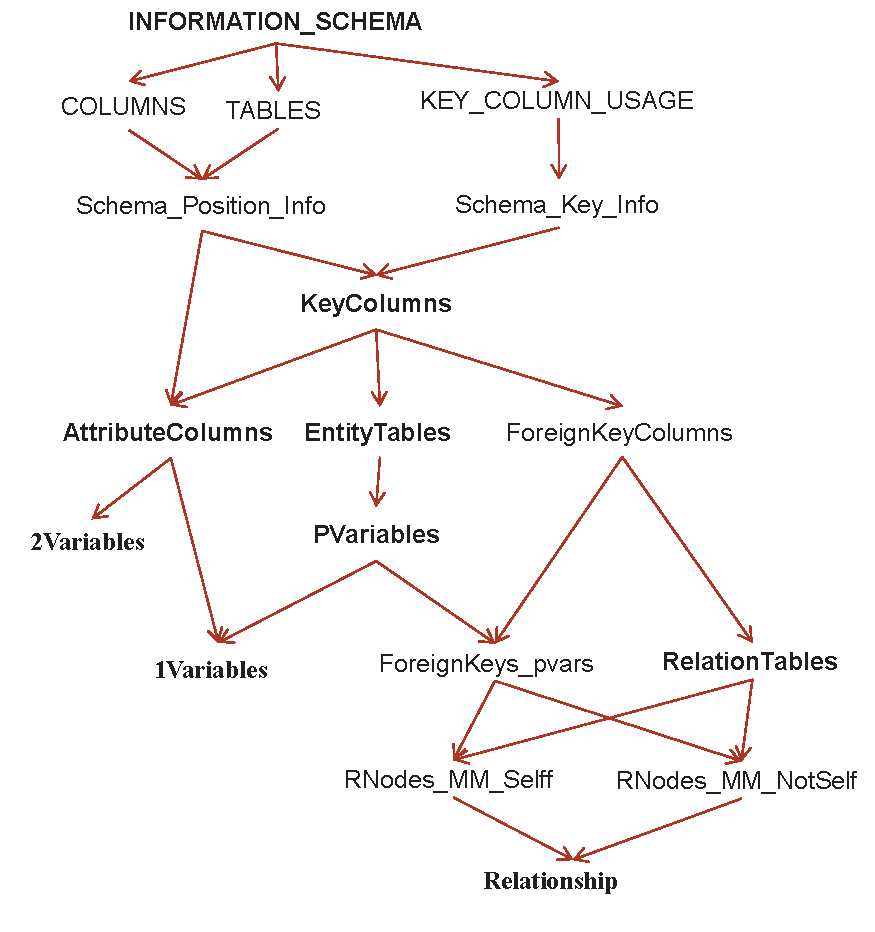
\includegraphics[width=0.5\textwidth]{rv_db.pdf} %move to the appendix
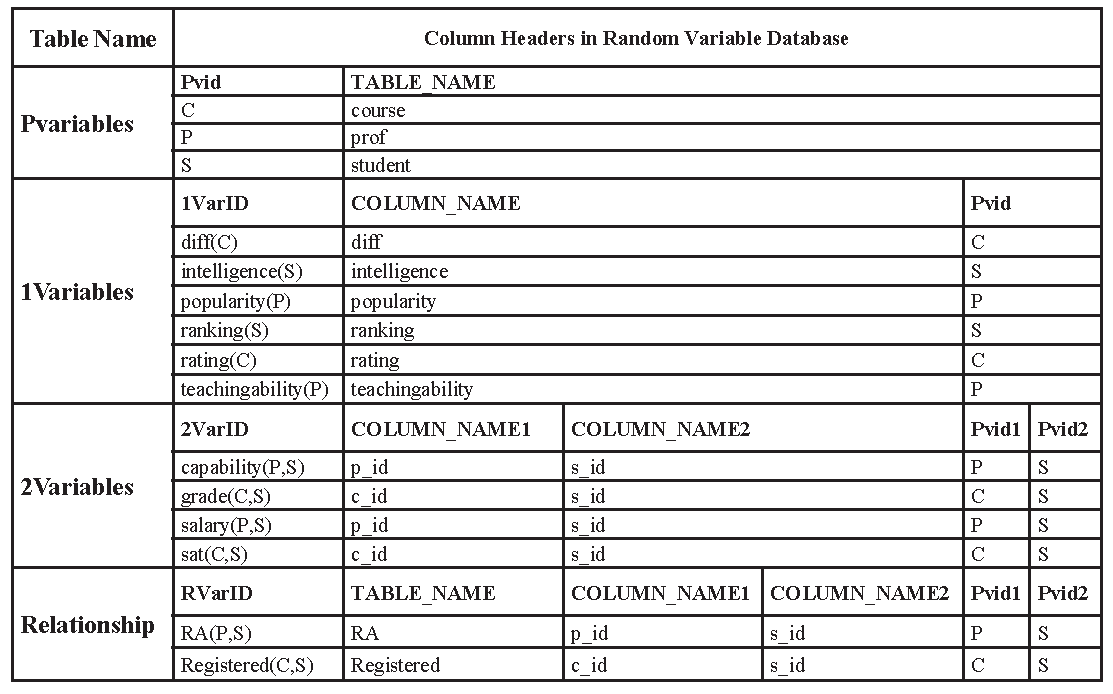
\includegraphics[width=0.5\textwidth]{rv_db_tables.pdf}
}
\caption{Main Tables in the Random Variable Database $\RVD$.
\label{fig:rv_db}}
\end{center}
\end{figure}

\section{The Count Manager} 
A key service for machine learning that a data management system needs to provide is counting how many times a given pattern is instantiated in the data. Such counts are known as {\em sufficient statistics} \cite{Graefe1998}. Many statistical machine learning algorithms do not require full access to the original data, but only to sufficient statistics (hence the name ``sufficient''). So if a database management system is extended to provide sufficient statistics on demand, a learning algorithm for single-table data can be applied to relational database with few modifications. 

There are several strong reasons for employing an RDBMS for gathering sufficient statistics. (1). The learning system saves expensive data transfer by executing count operations in the database server space rather than local main memory. (2) SQL optimizations for aggregate functions such as SUM and COUNT can be leveraged. (3) Sufficient statistics can be computed once and stored/cached for future reuse in the RDBMS. For many datasets, the number of sufficient statistics runs in the millions and is too big for main memory \cite{Moore1998}.  An RDBMS provides disk storage and fast access for large numbers of sufficient statistics. Previous work has exploited these advantages for single-table data \cite{Ordonez2010}. We discuss how to compute sufficient statistics for a more general situation where sufficient statistics combine information {\em across} different tables in the relational database. In SQL terms, this requires combining aggregate functions with table joins. 


\subsection{Relational Contingency Tables}
%Our starting point is the observation that a statistical learning algorithm like a Bayes net learner does not require an enumeration of individuals tuples, but only {\em sufficient statistics} \cite{Heckerman1995,Schulte2011}. 
%It is well-known in machine learning that a statistical learning algorithm like a Bayes net learner does not require an enumeration of individuals tuples, but only {\em sufficient statistics} \cite{Heckerman1995,Schulte2011}. 
Sufficient statistics can be represented in {\em contingency tables} as follows \cite{Moore1998}. 

 %A contingency table is defined as follows.
%The Bayes net is learned from the contingency table. 

%The count column in the $\ct$-table represents the number of instantiations for a given tuples of values in a row in the input database. 

Consider a fixed list of relational variables.
%$\R_{1}, R_{2},\ldots,R_{m}$, and attribute nodes $\functor_{1},\ldots,\functor_{j}$. 
A \textbf{query} is a set of $(variable = value)$ pairs where each value is of a valid type for the variable. 
The \textbf{result set} of a query in a database $\D$ is the set of instantiations of the population variables such that the query evaluates as true in $\D$.
For example, in the database of Figure~\ref{fig:instance} the result set for the query 
%$(\it{intelligence}(\S) = 2$, $\it{rank}(\S) = 1$, $\it{rating}(\C) = 3$, $\it{diff}(\C) = 1$, $\reg(\S,\C) = F)$
$(\it{intelligence}(\S) = 2$, $\it{rank}(\S) = 1$, $\it{popularity}(\P) = 3$, $\it{teachingability}(\P) = 1$, $\ra(\P,\S) = T)$ 
is the singleton $\{\langle \it{kim}, \it{Oliver}\rangle\}$. 
% $\{\langle \it{kim}, \it{101}\rangle\}$
The \textbf{count} of a query is the cardinality of its result set. 

Every set of variables $\set{V} = \{\V_{1},\ldots,\V_{n} \}$ has an associated \textbf{contingency table} denotes by $\ct(\set{V})$. %$CT(\set{V})$. 
This is a table with a row for each of the possible assignments of values to the variables in $\set{V}$, and a special integer column called $\qcount$. 
The value of the $\qcount$ column in a row 
corresponding to $V_{1} = v_{1},\ldots,V_{n} = v_{n}$ records the count of the 
corresponding query. 
Figure~\ref{fig:ct} shows the contingency table from university database. 
%The value of a relationship attribute is undefined for entities that are not related.
%Following \cite{Milch2007}, %\cite{BLOG}, 
%%$\it{capability(\P,\S)} = n/a $
%we indicate this by writing 
%%$\it{grade}(\s,\c) = n/a$ 
%$\it{capability(\P,\S)} = n/a $ for a reserved constant $\it{n/a}$. 
%The assertion $\it{capability(\P,\S)}$ = n/a is therefore equivalent to the assertion that $\ra(\P,\S) = \false$.
%For example, if student $\s$ is not registered in course $\c$, the value of $\it{grade}(\s,\c)$ is undefined. 


\begin{figure}[htbp]
\begin{center}
\resizebox{0.5\textwidth}{!}{
%%!%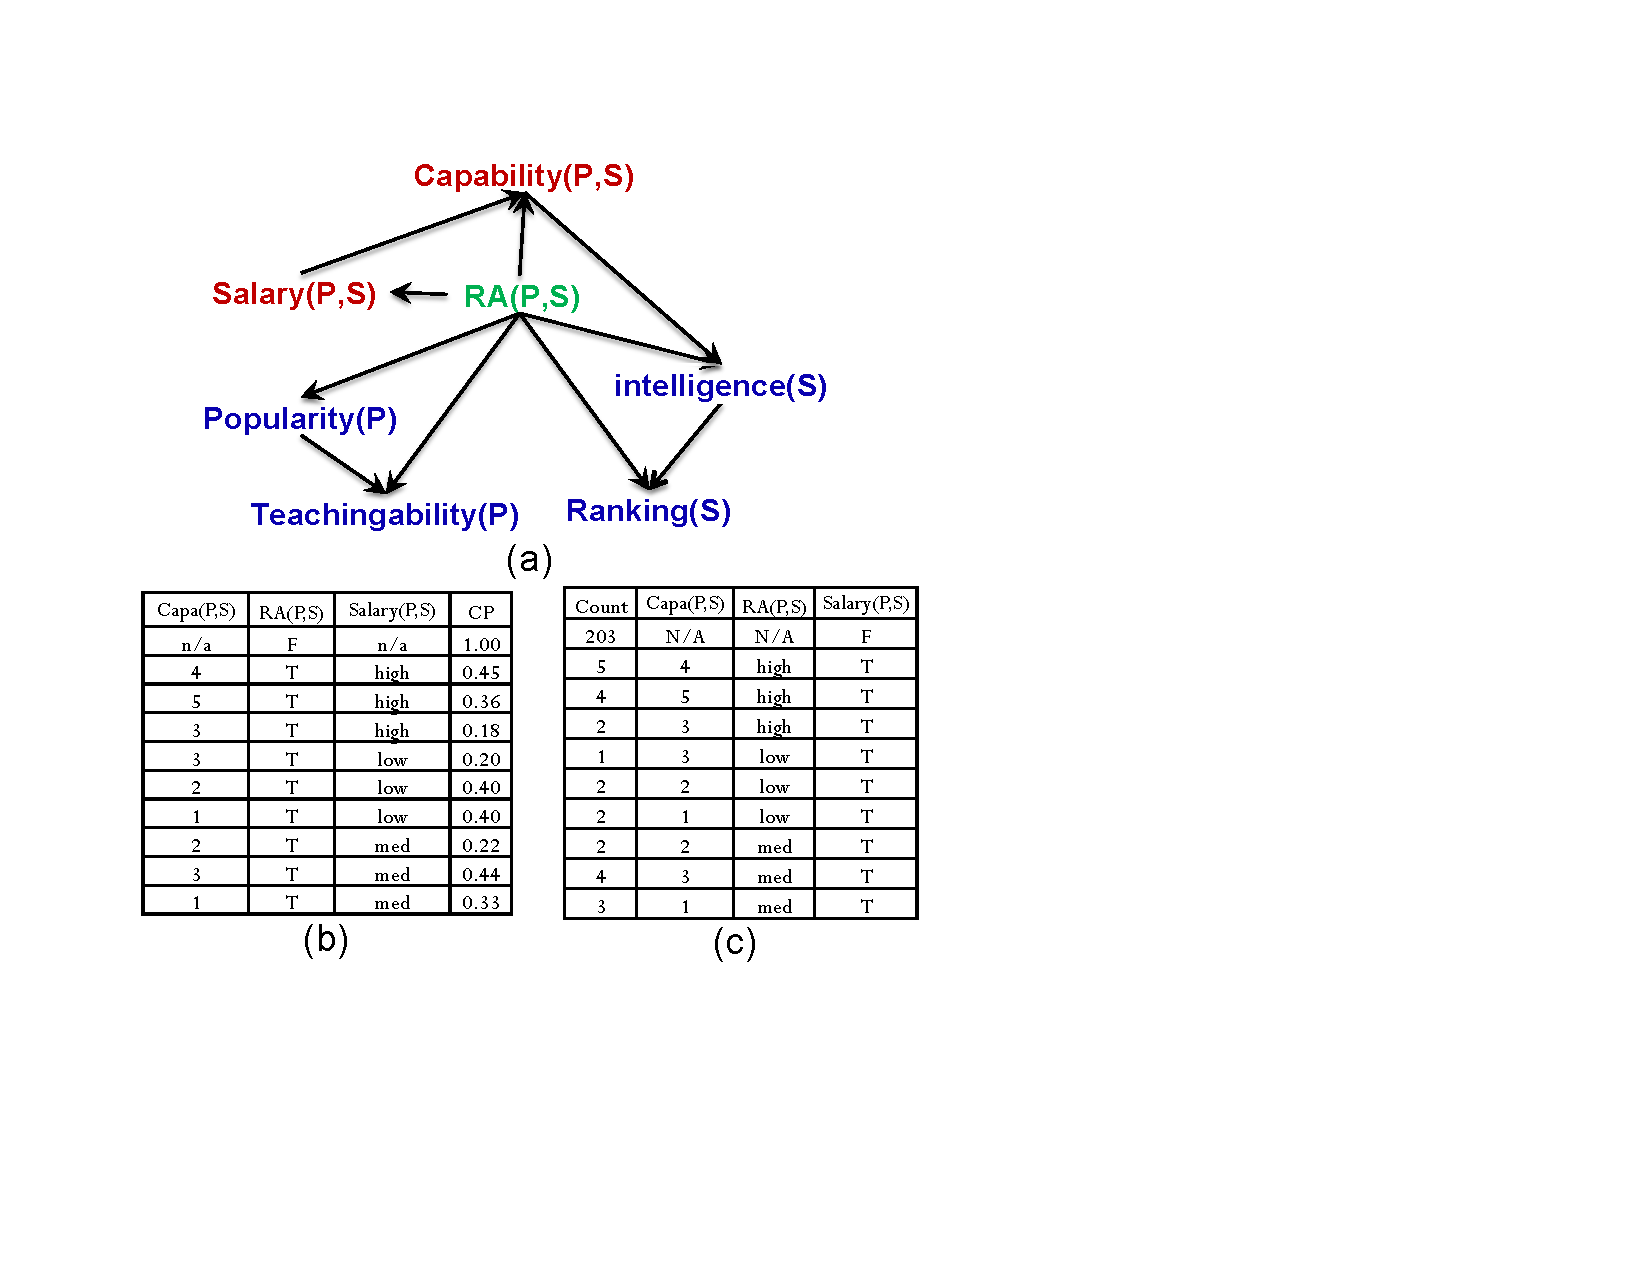
\includegraphics[width=1\textwidth]{pbn}
%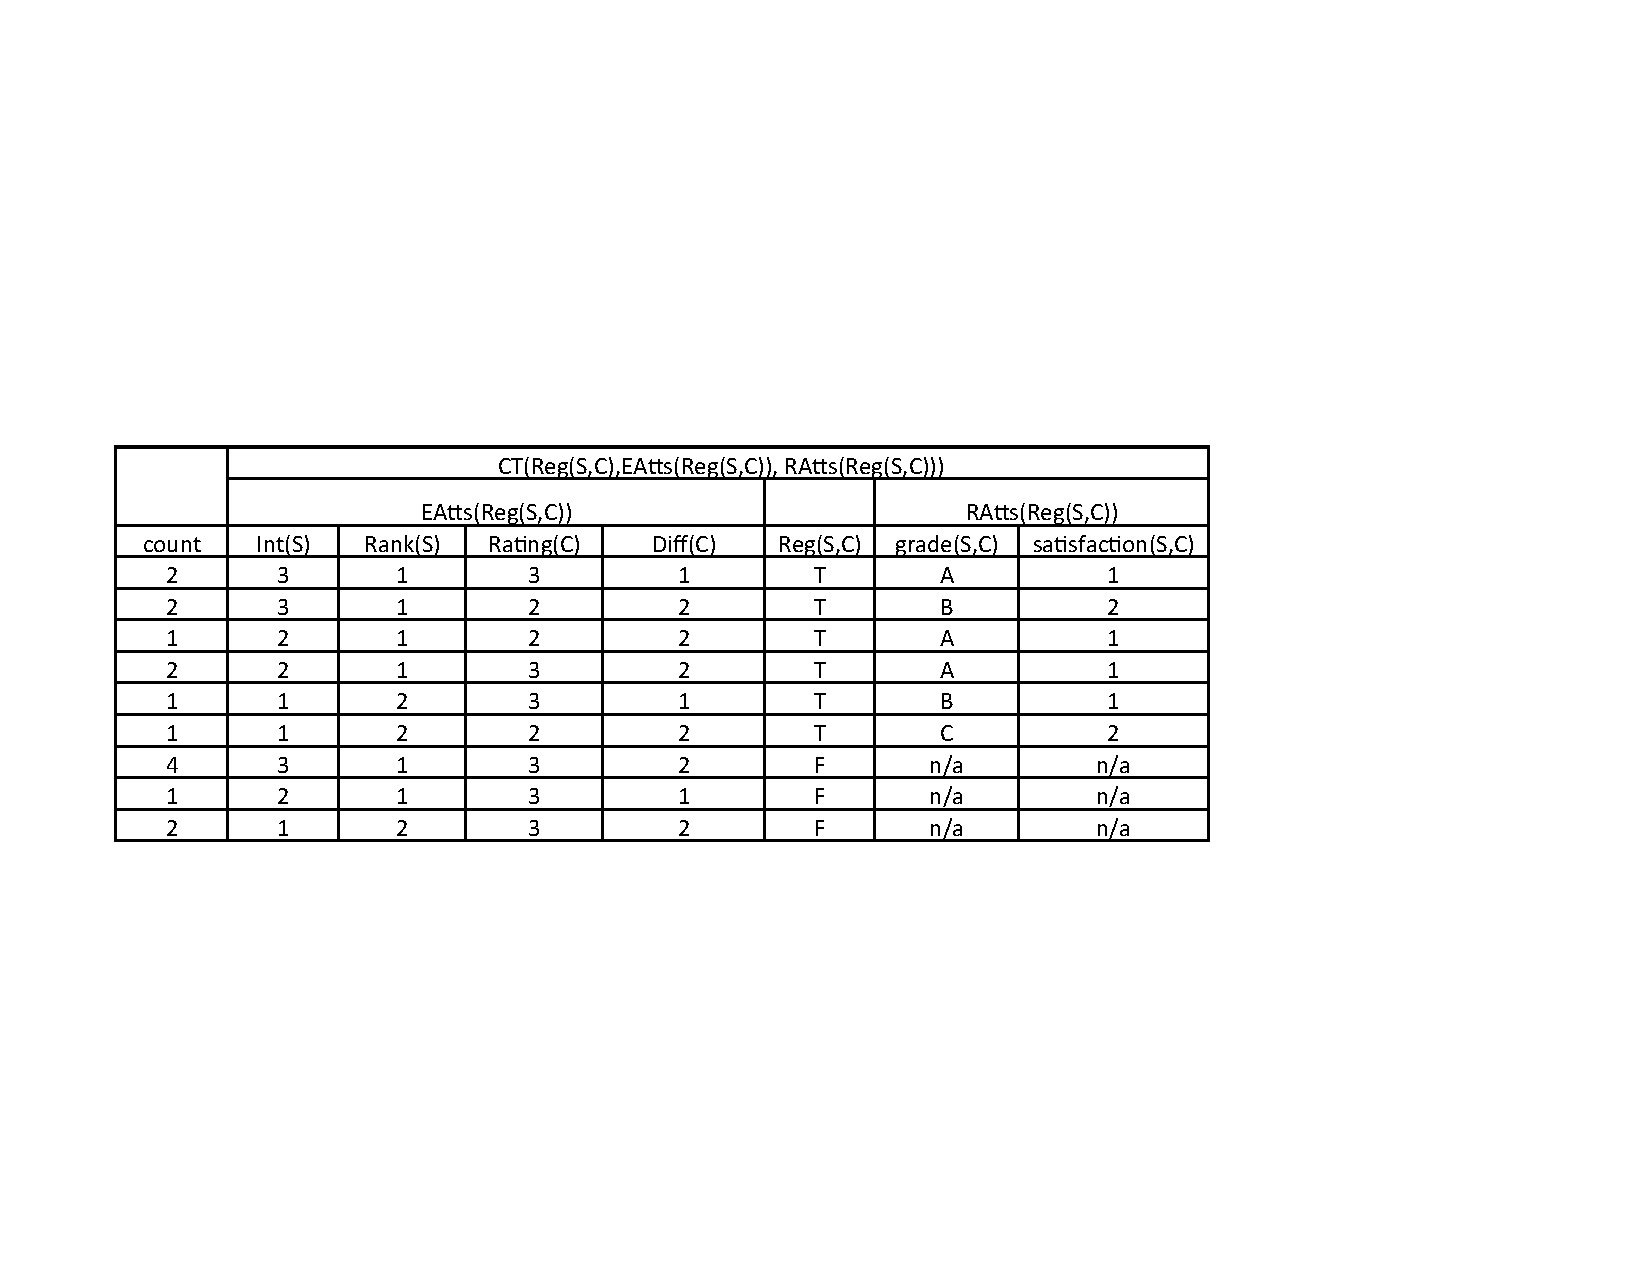
\includegraphics{figures/ct-table.pdf}
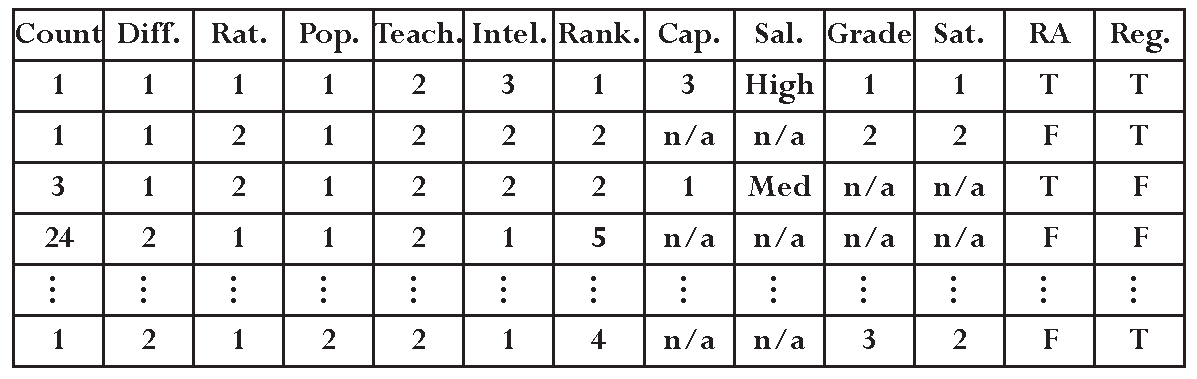
\includegraphics[width=0.5\textwidth]{uni-ct-table.pdf}
}
\caption{The contingency table for university database. % for the attribute-relation table of Figure~\ref{fig:university-tables}
Each row shows a query and its instantiation count in the database.
%one possible assignment of such variables with its count. 
% where for illustration we have added counts for another student like Jack and another course like 103.
%use partial real table
\label{fig:ct}}
\end{center}
\end{figure}

%A \textbf{conditional contingency table}, written 
%$$\ct(V_{1},\ldots,V_{k}|V_{k+1} = v_{k+1},\ldots, V_{k+m} = v_{k+m})$$
%is the contingency table whose column headers are $V_{1},\ldots,V_{k}$ and whose counts are  defined by subset of instantiations that match the conditions to the right of the $\vert$ symbol.  %  \textbar 

The \textbf{contingency table problem} is to compute a contingency table for a target set of variables $\set{V} $ and a given database $\D$. Machine learning algorithms can leverage this capability in several different ways. A pre-counting approach computes a joint contingency table for all relational random variables at once \cite{Moore1998,Qian2014a}. Another possibility is to use postcounting \cite{lv2012}: Rather than precompute a large contingency table prior to learning, compute many small contingency tables for  small subsets of variables on demand during learning. In this paper, we describe an approach to compute contingency tables that leverages SQL capabilities. First, we store contingency tables as first-class database tables, as in \cite{Qian2014a}. The column headers of a contingency table are IDs for the relational random variables, plus an integer-valued count column. Second, we use SQL queries to perform the necessary table joins and count operations. 



To illustrate the SQL-based approach, we examine the following problem: precomputing a contingency table for all relational random variables that are associated with a given chain of relationships. A relationship chain is a list $$[\Relation_{1}(\argterms_{1}),\ldots,\Relation_{k}(\argterms_{k})]$$
 of relationship variables such that each relationship variable shares at least one first-order variable with the preceding terms. In SQL terms, a relationship is formed by following foreign key pointers from one relationship table to the next. Sufficient statistics for relationship chains are important for discovering correlations between the attributes of entities that are related by paths of a certain type \cite{Getoor2007c} (called ``metapaths'' in \cite{Sun2012}). 
 
\subsection{Contingency Tables in SQL} \textbf{OS: this can be extended to include contingency tables with negative relationships}. The \textbf{Count Database} (CDB) stores a set of contingency tables each defined as a view. We discuss how to create these views using SQL.  
Each row in a contingency table represents the count for a conjunctive query in a logical calculus; we refer to these as count-conjunction queries.
It is well-known that conjunctive queries in a logical calculus can be algorithmically translated into relational algebra queries and hence into an SQL query \cite{Ullman1982}. Our approach uses SQL itself to construct the count-conjunction query. We refer to this construction as an SQL \textbf{meta query}. The meta query approach has several advantages over using a general programming language. (1) Succinctness and portability: Given the metainformation in the random variable database, the meta query is short, mainly requires a few natural joins. The meta query requires only standard SQL, whereas a translation in an application language (e.g., Java) would have to be ported for each different application language. (2) Automatic Update: We can store the result of the meta query as a database view. This means that changes in the original database schema are propagated to contingency tables. For instance, if a column $\it{gpa}$ is added to the $\it{Student}$ table in the original database schema, then the view definition adds this column automatically to contingency tables derived from the $\it{Student}$ table.

A contingency table for a set of random variables can be computed by an SQL count-conjunction query of the form 
\begin{alltt}
CREATE ct-table(variables) AS
SELECT COUNT(*) AS count, <VARIABLE-LIST>
FROM TABLE-LIST
GROUP BY VARIABLE-LIST
WHERE <Join-Conditions>
\end{alltt}
%As the top level of  Figure~\ref{fig:flow} illustrates, 
%The required counts involving only true relationships can be computed using the standard SQL constructs COUNT(*) and GROUP BY. 
%The general form of these operations is the same for every input database. 
%The varying part is the list of columns to be included, which depends on the input database. 
%For a fixed database, the column lists can be hard-coded. 
%To achieve a general solution when the column list is not known in advance, we introduce a new approach that we refer to as an SQL \textbf{meta query}. 

%Thus an SQL meta query maps schema information to the components of another SQL query. 
 Given a list of $\RRV$'s as input, the meta query is constructed as follows. 
\begin{description}
\item[FROM LIST] Find the tables referenced by the $\RRV$'s. An $\RRV$ references the entity tables associated with its population variables (see $\RVD.Pvariables$). Relational $\RRV$'s also reference the associated relationship table (see $\RVD.Relationship$). 
\item[WHERE LIST] Add join conditions on the matching primary keys of the referenced tables in the WHERE clause. The primary key columns are recorded in table $\RVD.KeyColumns$. 
\item[SELECT LIST] For each attribute $\RRV$, find the corresponding column name in the original database (see $\RVD.AttributeColumns$). Rename the column with the ID of the $\RRV$.
\end{description}

We represent a count-conjunction query of this form in 
four kinds of tables: the Select, From, Where and Group By tables. The Select table lists the entries in the Select clause of the target query, the From table lists the entries in the From clause, and similar for Where and GROUP BY tables. The entries of the Group By table (not shown) are the same as the Select table without the $\qcount$ column.
Given the four query tables, the corresponding SQL count query can be easily executed in an application or stored procedure to produce the $\ct$-table entries.
Figure~\ref{fig:meta-query} shows an example of metaqueries for the university database. The metaquery accesses tables in the Relational Random Variable Database. %We omit further details due to space constraints.

\begin{figure}[htb]
\begin{center}
\resizebox{0.5\textwidth}{!}{
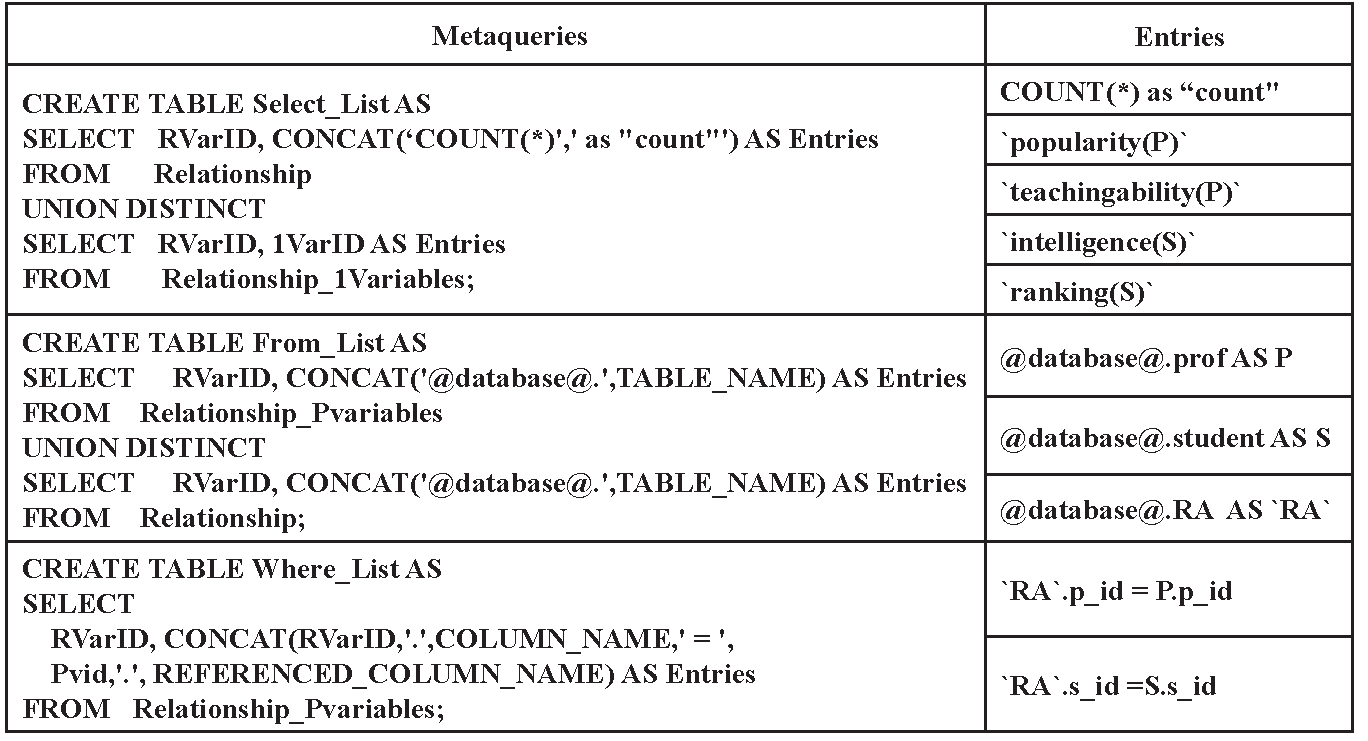
\includegraphics[width=0.5\textwidth]{meta-query.pdf}
}
\caption{Example of metaqueries and metaquery results for the random variable list 
%relationship table $\ra$  
based on university database. The $\it{@database@}$ is a string placeholder for the input database name. 
~\label{fig:meta-query} }
\end{center}
\end{figure}







%Relational learning algorithms explore longer and longer chains of relationships that may link statistically dependent objects. 
%Chains of relationships form a natural lattice structure. 
%%Conceptually, the lattice view simplifies describing and developing learning algorithms. Computationally, 
%The Virtual Join algorithm computes contingency tables by using the results for smaller relationships for larger relationship chains. In terms of the lattice, this corresponds to moving from the bottom to the top. 
%%The lattice diagram facilitates the computation of contingency tables that summarize the sufficient database statistics for learning.
%%
%%\subsection{The Relationship Lattice}
%%
%
%A relationship set is a \textbf{chain} if it can be ordered as a list $[\Relation_{1}(\argterms_{1}),\ldots,\Relation_{k}(\argterms_{k})]$ 
%%is a \textbf{chain} if 
%such that each functor $\Relation_{i+1}(\argterms_{i+1})$ shares at least one population variable with the preceding terms $\Relation_{1}(\argterms_{1}),\ldots,\Relation_{i}(\argterms_{i})$.
%%\footnote{Essentially the same concept is called a slot chain in PRM modelling \cite{Getoor2007c}.}
%%A relationship set forms a chain if the corresponding list is a chain. 
%All sets in the lattice are constrained to form a chain.
%%
%For instance, in the University schema of Figure~\ref{fig:university-schema}, a %relationship 
%chain is formed by the two relationship nodes
%\[\reg(\S,\C),\ra(\P,\S).\]
%%list \[[\it{RA}(\P,\S),\it{Registered}(\S,\C)].\] 
%If relationship node $\it{Teaches}(\P,\C)$ is added,
%%to record which student is a TA for which course,
%we may have a three-element chain \[\reg(\S,\C),\ra(\P,\S),\it{Teaches}(\P,\C).\] 
%The subset relation defines a lattice on relationship sets/chains. 
%Figure~\ref{fig:big-lattice} illustrates the  lattice for the relationship nodes in the university schema. 
%For reasons that we explain below, entity tables are also included in the lattice and linked to relationships that involve the entity in question. 
%
%\begin{figure}[htbp]
%\begin{center}
%\resizebox{0.5\textwidth}{!}{
%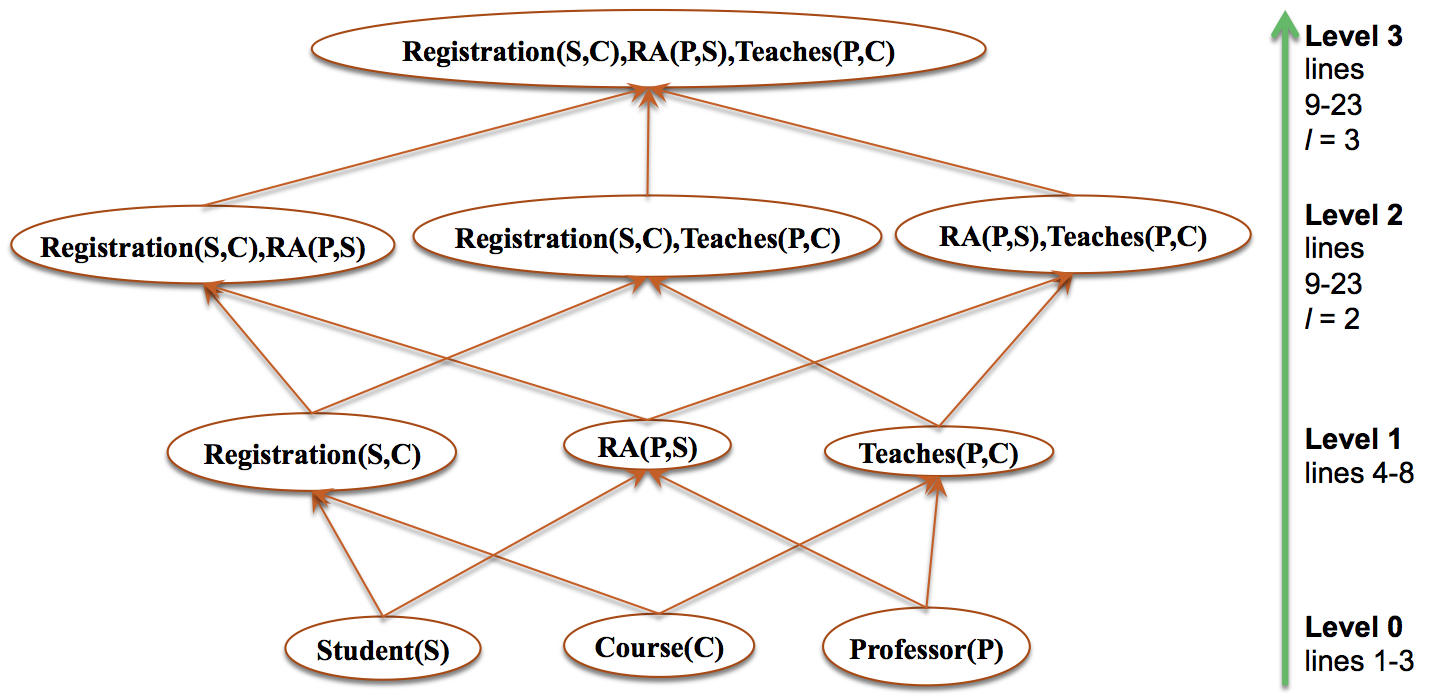
\includegraphics[width=0.8\textwidth]{figures/uni-big-lattice.png}
%}
%\caption{A lattice of relationship sets for the university schema of Figure~\ref{fig:university-schema}.
% Links from entity tables to relationship tables correspond to foreign key pointers. 
%%The list representation of the sets is determined by the functor ordering $\it{Registered} < \it{TA} < \it{Teaches}$. 
%\label{fig:big-lattice}}
%\end{center}
%\end{figure}
%
%
%
%
%With each relationship set $\set{\Relation}$ is associated a $\ct$-table $\ct_{\set{\Relation}}$. 
%For a relationship chain $\set{\Relation}$ the nodes in the $\ct$-table  $\ct_{\set{\Relation}}$%$\B_{\set{Relation}}$
% comprise: the Rnodes in the set $\set{\Relation}$, the 1Nodes and 2Nodes associated with each of the Rnodes. To describe these, we introduce the following notation.
%%Let's first introduce the notations for all kinds of functor nodes in order to extend relational algebra operators for manipulating $\qcount$ in contingency tables as follows.
%%Let $R$ be a relationship node and let $\set{R}$ be a set of relationship nodes.
%
%\begin{itemize}
%\item $\eatts(R)$ denotes the set of entity attribute nodes for the population variables involved in the relationship $R$. 
%\item $\eatts(\set{R})$ is the union of the entity attributes for each relationship $R \in \set{R}$.
%\item $\ratts(R)$ denotes the set of relationship attribute nodes for %the population variables involved in 
%the relationship $R$.
%\item $\ratts(\set{R})$ is the union of the relationship attributes for each relationship $R \in \set{R}$.
%\item $\atts(R)$ is the set of both entity and relationship attributes for relationship $R$, similarly for $\atts({\set{R}})$.
%\item  $1Nodes(\A)$ denotes the attributes of a population variable $\A$ collectively
%%\item $R_{i}$ is the Boolean relationship node.
%%\item $\etable$ denotes a entity table.
%%\item $Column\_List({\etable})$ is the set of non-count columns in entity table $\etable$.
%\end{itemize}
%
%In this notation, the nodes in the $\ct$-table  $\ct_{\set{\Relation}}$  are denoted as $\set{\Relation} \cup \atts({\set{R}})$. 
%
%\emph{Implementation.} The Random Variable Database specifies the set of relationship nodes for building the lattice. Building a lattice of relationship chains can be done using any standard technique, such as those developed for enumerating itemsets in association rule  mining \cite{Agrawal1994}. 
%We create a table {\em Lattice} in the Bayes net database with one row for each relationship chain. We also create two auxilliary tables: One that lists which relationship chains are children of which others. A child contains exactly one more relationship node (cf. Figure~\ref{fig:big-lattice}). 
%%For example, the relationship chain $\it{Registered}(\S,\C),\it{RA}(\S,\P)$ is a child of the chain $\it{Registered}(\S,\C)$. Another auxilliary table lists which relationship nodes are members of which relationship chain. For example, the relationship chain $\it{Registered}(\S,\C),\it{RA}(\S,\P)$ has two members. The auxilliary tables are used during learning as described below.
%
%The goal of the Virtual Join Algorithm is to compute a contingency table for each point in the lattice. 
%In the example of Figure~\ref{fig:big-lattice}, the algorithm computes 10 contingency tables. The $\ct$-table for the top element of the lattice is the $\ct$-table for the entire database. 
%It is useful to distinguish two types of rows within each $\ct$-table: rows where all the relationship nodes are assigned the value $\true$---positive relationships only---and rows where one or more relationship nodes are assigned the value $\false$---some negative relationships. 
%We begin with the case of positive relationships.

\section{The Model Manager}

There is a large space of machine learning models, which require support for a diverse set of capabilities. We focus on three services that are required in almost all model selection tasks: 1) Estimating and storing parameter values. 2) Computing one or more model selection scores. 3) Inferring a model prediction for a set of test instances and scoring the model against the true values. We briefly discuss other more advanced capabilities, such as model structure learning, and incorporating user background knowledge. 

In machine learning theory and implementations, different objects are often represented as matrices, and combined using matrix multiplication. The same results can be obtained in a relational format using natural joins with summations \cite{regina}, as we illustrate in several examples below.

Our illustrative case study describes how MRLBase can be used to implement a challenging machine learning application: Constructing a Bayesian network model for a relational database. Managing Bayesian networks are a good illustration of typical challenges and how RDBMS capabilities can address them because: (1) The structure of a Bayesian networks is fairly complex, based on a graph of relational random variables. (2) BN parameters are localized and not simply a flat vector. (3) Bayesian networks are widely regarded as a very useful model class in machine learning and AI, that supports decision making and reasoning under uncertainty. At the same time, they are considered challenging to learn from data. (4) Database researchers have proposed Bayesian networks for combining databases with uncertainty \cite{bayestore,graepel}. After we have illustrated the capabilities of our SQL-based approach, we discuss how to apply it with other machine learning models, such as classifiers.

\subsection{Bayesian Networks for Relational Data}
A {\bf Bayesian Network (BN)} is a directed acyclic graph (DAG) whose nodes comprise a set of random variables and conditional probability parameters.
The parameters of the BN  
are the conditional probabilities of the form, $P(\it{child}|\it{parent\_values}$), that specify the probability of a child node value given an assignment of values to its parents. 
In this paper we consider only Bayesian networks whose nodes are relational random variables (called ``Parametrized Bayesian Networks'' in \cite{Poole2003}). 
%If a Parametrized random variable appears in a Bayes net, we often refer to it simply as a node. 
Figure \ref{fig:pbn} shows a Bayesian network for the University domain (only considering the $\ra$ relationship for simplicity.) 
\begin{figure}[htbp] %  figure placement: here, top, bottom, or page
 \centering
\resizebox{0.4\textwidth}{!}{
 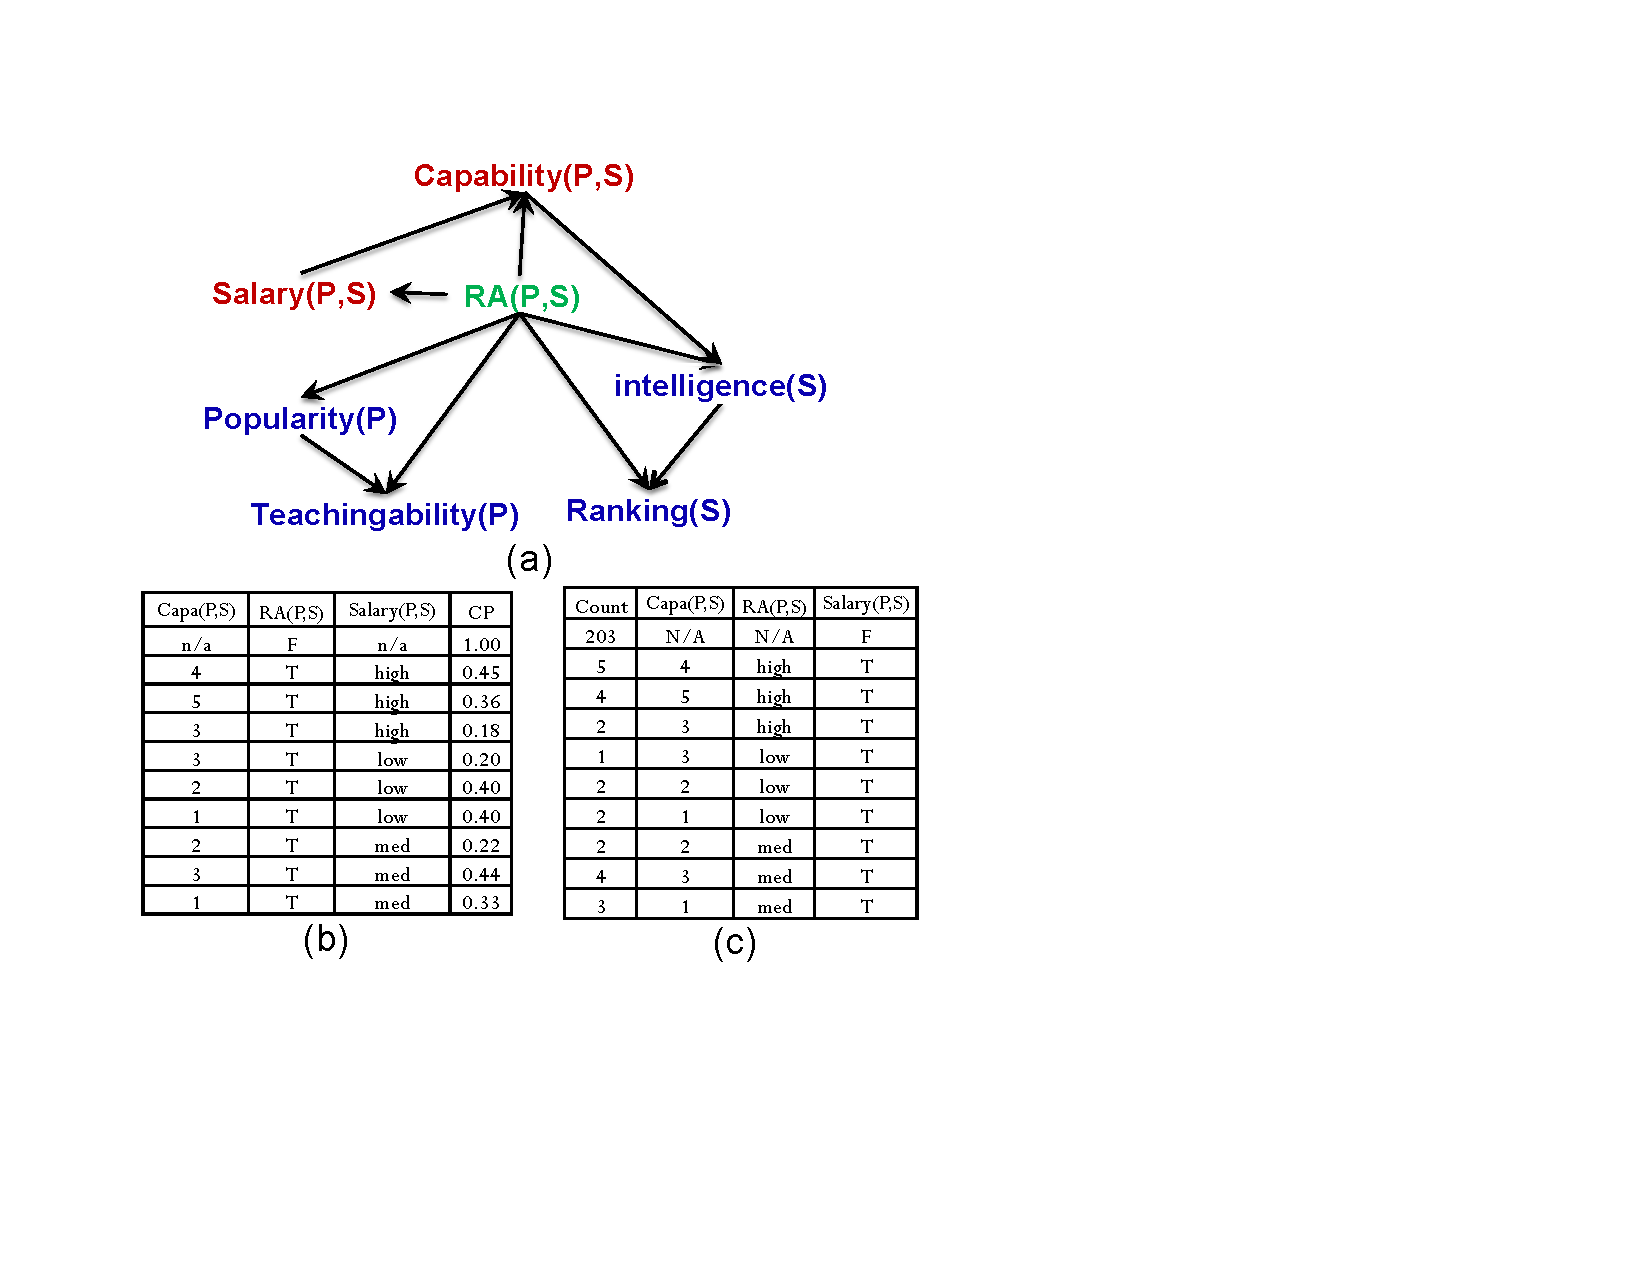
\includegraphics[width=0.5\textwidth]{pbn.pdf} 
} 
\caption{(a) Bayesian network for the University domain. (b) Conditional Probability table $Capability(\P,\S)\_\cptable$, for the node $Capability(\P,\S)$. Only value combinations that occur in the data are shown. (c) Contingency Table $Capability(\P,\S)\_\cttable$ for the node $Capability(\P,\S)$ and its parents. Both CP and CT tables are stored as database tables in the DBMS.
}
 \label{fig:pbn}
\label{fig:ct-cp-table}
\end{figure}


%\begin{figure}[htbp] %  figure placement: here, top, bottom, or page
% \centering
%\resizebox{0.4\textwidth}{!}{
% \includegraphics[width=0.5\textwidth]{ct-cp-table.pdf} 
%} 
%\caption{ct-cp-table}
% \label{fig:ct-cp-table}
%\end{figure}

%\subsection{Model Representation} 
\paragraph{SQL Representation of Model Structure} A Bayesian network structure is a directed graph that can be stored straightforwardly in a database table $\it{BayesNet}$ whose columns are $\it{child}$ and $\it{parent}$. The table entries are the IDs of relational random variables defined in the Relational Random Variable database. An entry such as $(\it{Capability}(\P,\S),\it{Salary}(\P,\S),)$ means that $\it{Capability}(\P,\S)$ is a child of $\it{Salary}(\P,\S)$. This table is stored in the \textbf{Models Database}, abbreviated as $\MDB$. The relational schema for the Models Database is shown in Table~\ref{table:mdb-schema}.

\begin{table}[tbp] \centering
 \begin{tabular}
[c]{|l|}\hline
$\it{BayesNet}$(\underline{$child$,$parent$})\\
$\it{@nodeID@\_\cptable}$(\underline{$@nodeID@$,$parent_{1},\ldots,parent_{k}$},\cpcol)\\ 
$\it{Scores}$(\underline{$nodeID$},$\loglikelihood$,$\parameters$,$\aic$)\\
\hline
\end{tabular}
\caption{The main tables in the Models Database $\MDB$. For a Bayesian network, the Models Database stores its structure, parameter estimates, and model selection scores.The $\it{@nodeID@}$ expression ranges over the different IDs of Bayesian network nodes (random variables), for instance $\it{Capability}(\P,\S)$.
\label{table:mdb-schema}} 
\end{table}



\subsection{Parameter Manager}

To make predictions with a model, we need to estimate values for its parameters. In keeping with our approach of storing all model components in the RDBMS, the parameters for a Bayesian network are stored as database tables, called conditional probability tables. Conditional probability tables have the same structure as contingency tables, but with a special column $\cp$ instead of $\it{count}$. Maximizing the data likelihood is the basic parameter estimation method for Bayesian networks. It can be shown that the maximum likelihood estimates use the observed frequency of a child value given its parent values. 

\paragraph{SQL Construction of Conditional Probability Tables} Given the sufficient statistics in a contingency table, a conditional probability table containing these frequencies can be computed using SQL as follows.

\begin{enumerate}
\item For each node, construct a local contingency table whose variable set comprises the node and its parents. This table can be computed from scratch using the count manager, or may already be available as part of model structure learning (see below). 
\item Using a SUM(count) = parent\_count and GROUP BY query on the local contingency table, construct a  parent contingency table whose variable set comprises the parents only.
\item Carry out a natural join of the local contingency table with the parent contingency table, dividing each local contingency count by the parent\_count. The natural join matches the values of parent variables. 
\end{enumerate}

All of these tables can be stored as views. This means that parameter values are updated automatically when contingency tables are updated, that is, when new data are obtained. 
Figure~\ref{fig:ct-cp-table} shows a local contingency table and a conditional probability table for the node Capability(P, S). More complex smoothing methods such as the Laplace correction can be easily computed from the maximum likelihood estimates.

\subsection{Model Score Computation}

Model structure learning uses a model selection score to find an optimum model for a given database. Model selection scores can be computed and stored in an RDBMS as well. Caching model selection scores is important for scalable structure learning \cite{tetrad}. A typical model selection approach is to maximize the likelihood of the data, balanced by a penalty term. For instance, the Akaike Information Criterion (AIC) is defined as follows.
\[
\mathit{AIC}(\G,\datatable) \equiv ln(P_{\widehat{G}}(\datatable)) - \parameters(\G) \]
where $\widehat{G}$ is the BN $\G$ with its parameters instantiated to be the maximum likelihood estimates given the datatable $\datatable$, and $\parameters(\G)$ is the number of free parameters in the structure $\G$. This expression involves two terms, the likelihood and the number of parameters. 
%We discuss how to use SQL for computing each.

Assume that the maximum likelihood estimates are represented in a conditional probability table as discussed above. For a BN, the likelihood function can be computed node by node, as follows. For each child node value, and for each combination of parent values: (1) find the instantiation count in the data for the conjunction of child node value and parent node values. (2) Find the conditional probability of the child node value given the parent node values. (3) Multiply the instantiation count by the logarithm of the conditional probability. Finally, sum these products to obtain a total likelihood score for the child node.

The number of parameters for a node is basically the product the possible values for the parent nodes, multiplied by (the number of the possible values for the child node -1). One complication is that if a relationship node has the value $\false$, then all associated 2Variables (relationship attributes) must have the value n/a. The computation of the number of parameters must be adjusted to account for this deterministic relationship; for the details see the script in the supplementary material. 

\paragraph{SQL Computation of Model Score} We assume that for each node with ID $@nodeID@$, a conditional probability database table $@nodeID@\_\cptable$ has been built in the Models database $\MDB$. Similarly, we assume that
a local contingency database table $\CDB.@nodeID@\_\cttable$ has been built in the Count Database $\CDB$ (see Figure~\ref{fig:ct-cp-table}). The model likelihood for node $@nodeID@$ can be computed in SQL simply using the natural join of the two tables summing over a row-wise product, as follows.


\begin{alltt}
SELECT @nodeID@,  SUM
(@nodeID@\_\cptable.\cpcol * \CDB.@nodeID@\_\cttable.\countcol) AS \loglikelihood
FROM @nodeID@\_\cptable NATURAL JOIN \CDB.@nodeID@\_\cttable
\end{alltt}

The $\loglikelihood$ value for $@nodeID@$ is inserted into the $\it{Scores}$ table. 

%our system creates a view $@nodeID@\_Likelihood$. This view has the same schema as the CP database table $@nodeID@\_\cptable$, except that instead of a conditional probability for a given child-parent configuration, we store a likelihood score. 

%We assume that a local contingency database table $\ct$ and a conditional probability database table $\cptable$ have been built for the child node as describe above (see Figure~\ref{fig:ct-cp-table}). The model likelihood can be computed in SQL simply as the natural join of the two tables, with a new column $\it{likelihood}$ defined by $$\it{likelihood} = \it{ct.count} * log(\cptable.\cp).$$ 

For determining the number of parameters, the number of possible variable values can be found in the $\it{Domain}$ table of the Random Variable Database $\RVD$.  The $\parameters$ number for $@nodeID@$ is also inserted into the $\it{Scores}$ table. The AIC column is then defined as $\aic = \loglikelihood - \parameters$. These values can be inserted directly or the AIC column can be implemented as a derived column. %Given the table $\it{BayesNet}$ that specifies the Bayes net graph, we create a view $\it{NumParameters}$ whose columns are $\it{Node}$ and $\it{Parameters}$. An entry such as $(\it{Capability}(\P,\S),16)$ means that the number of parameters associated with the capability node in the BN model is 16. 
%
Other model selection scores such as BIC and BDeu can be computed in a similar way given the model likelihood and number of parameters.

\subsection{Structure Learning}
 


- structure learning for Bayesian network. 
- basic: use big CT-table, learn BN.
- if big Ct-table doesn't fit in main memory, then you can use DBN to score.
- hierarchical search learn-and-join.



\section{Test Set Predictions}

A basic procedure for evaluating the accuracy of a machine learning algorithm is the train-and-test paradigm, where the system is provided a training set for learning and then we test its predictions on unseen test cases. %
%
We first discuss how to compute a prediction for a single test case, then how to compute an overall prediction score for a set of test cases. A number of prediction models have been developed for multi-relational data \cite{Dzeroski2003}. A prominent model class is defined by a \textbf{log-linear equation}

$$P(\Y = \y|\set{\X} = \x) \propto \exp(\sum_{i} w_{i} \cdot f_{i}(\y,\x))  $$

where $\Y$ denotes a ground target node to be classified, $\y$ a class label, $\X = \x$ is an assignment of values $\x$ to predictors or input variables $\y$, a feature function $f_{i}$ maps the class label and input variable values to a real number, and $w_{i}$ is a weight parameter for the feature function $f_{i}$. The term ``ground'' refers to replacing population variables by target instances. For example, a ground target node may be $\it{intelligence}(jack)$, meaning that the goal is to predict the intelligence of student Jack. In this example, we refer to Jack as the \textbf{target entity}. A log-linear classification model is associated with the prominent Markov Logic Network model class (Tuffy, Domingos). A log-linear classification model for Bayesian networks can be defined as follows [cite]. For the class variable and for each child of the class variable, there is a feature for each joint assignment of values to child and parents. The associated feature function $f_{i}(\it{child\_value},\it{parent\_values})$ is the instantiation count for the conjunction of child and parent values, {\em given the target instance}. The weight parameter $w_{i} \equiv ln(P((\it{child\_value}|\it{parent\_values}))$ is the log-conditional probability stored in the BN parameter table. For instance, suppose that we want to use the BN of Figure~\ref{fig:ct-cp-table} to predict $\it{intelligence}(jack)$. One feature function in the log-linear equation would correspond to the conjunctive feature $$\it{intelligence}(jack) = hi,\it{capability}(\P,jack) = 1, \it{RA}(\P,Jack) = \true.$$ The feature function is the number of true instances of this query in the data, i.e. it is the number of capability scores 1 that Jack has earned for each professor that he has worked with (i.e., $\it{RA}(\P,Jack) = \true$). This number is multiplied by $\ln(P(\it{intelligence}(jack) = hi|\it{capability}(\P,jack) = 1, \it{RA}(\P,Jack) = \true)$. For further details please see ...

\paragraph{SQL Computation of the Log-Linear Classification Score}
The derivation of the log-linear equation for a BN shows that the conditional class probability is equivalent to the log-likelihood of a restricted BN and a restricted set of instantiation counts. The restrictions are that only the class node and its children are included in the log-likelihood computation, and all instantiations must agree with the target entity ($\S = Jack$). This observation means that we can apply the log-likelihood computation described in Section~\ref{sec:likelihood} as follows. %
(1) For the class node and each of its children, compute the $\cttable$ for instantiations that agree with the target entity. (2) For each such $\cttable$, compute the product with the associated $\cptable$ using the natural join as in Section~\ref{sec:likelihood}. As Figure~\ref{fig:test} illustrates, the computation is the same as for the general model log-likelihood. The new problem is finding the contingency table for the target entity. SQL allows us to solve this very easily by restricting counts to target entity in the WHERE clause. To illustrate, suppose we want to modify the contingency table query of Figure~\ref{fig:meta-query} to compute the contingency table for $\S = Jack$. First we add the student id to the SELECT clause, so the new SELECT clause becomes

\begin{alltt}
COUNT(*) AS count, popularity(P), teachingability(P),
intelligence(S), ranking(S), \em{S.sid}
\end{alltt}

and the new WHERE list becomes

\begin{alltt}
RA.p\_id = P.p\_id AND RA.s\_id = S.s\_id AND \em{S.s\_id = jack}.
\end{alltt}

We emphasize the new parts of the queries and omit apostrophes for readability. The FROM and GROUP BY clauses are the same as in Figure~\ref{fig:meta-query}. The metaquery of Figure~\ref{fig:meta-query} is easily changed to produce these SELECT and WHERE CLAUSES. 
In sum, the log-likelihood computation of Section~\ref{sec:likelihood} can be easily adapted to compute a log-linear classification score by adjusting the contingency table counts to the target entity. This is an example of how well the high-level SQL constructs support computation with structured objects. Programming the likelihood computations in a general programming language like Java requires significant development effort and results in a less concise and less portable solution. [move to likelihood section. This illustrates the modularity and reusability of solutions]

We next consider a setting where a model is to be scored against an entire test set. This occurs for instance in the standard cross-validation computation for model scoring. For concreteness, suppose the problem is to predict the intelligence of a set of students
 $\it{intelligence}(jack), \it{intelligence}(jill)$,

 $\it{intelligence}(student_{3}),\ldots, \it{intelligence}(student_{m})$.
 An obvious approach is to loop through the set of test instances, repeating the likelihood computation for each single instance. However, SQL supports {\em block access} where we process the test instances as a block. Intuitively, instead of building a contingency table for each test instance, we build a single contingency table that stacks together the individual contingency tables. Blocked access can be implemented in a beautifully simple manner in SQL: we simply add the primary key id field for the target entity to the GROUP BY list. To illustrate,  suppose that the $\it{Student}$ table contains all test target entities. The query for the stacked contingency table is constructed as in Figure~\ref{fig:meta-query}, with the change that: We add the $\it{S.sid}$ field to the SELECT and to the GROUP BY lists. The FROM and WHERE clauses are as in Figure~\ref{fig:meta-query}. This is an example of how well the high-level SQL constructs support computation with structured objects. Programming blocked access in a general programming language like Java would require significant development effort and probably new file or data structures. If the set of test instances is large, a stacked contingency table is also unlikely to fit into main memory.


\section{Evaluation} 
We describe the system and the datasets we used.
Code was written in Java, JRE 1.7.0.  and executed with 8GB of RAM and a single Intel Core 2 QUAD Processor Q6700 with a clock speed of 2.66GHz (no hyper-threading). The operating system was Linux Centos 2.6.32. 
The MySQL Server version 5.5.34 was run with 8GB of RAM and a single core processor of 2.2GHz. 
All code and datasets are available on-line (pointer omitted for blind review). 


\subsection{Datasets}
We used seven benchmark real-world databases. For detailed descriptions and  the sources of the databases, please see reference~\cite{Schulte2012}. Table~\ref{table:datasetsize} summarizes basic information about the benchmark datasets.  A  self-relationship %\cite{Heckerman+al:SRL07} 
relates two entities of the same type (e.g. $\it{Borders}$ relates two countries in Mondial). Random variables for each database were defined as described in Section~\ref{sec:variables} (see also \cite{Schulte2012}). IMDB is the largest dataset in terms of number of total tuples (more than 1.3M tuples) and schema complexity. %attributes.
It combines the MovieLens database\footnote{www.grouplens.org, 1M version} with data from the Internet Movie Database (IMDB)\footnote{www.imdb.com, July 2013} following \cite{Peralta2007}.

\begin{table}[hbtp] \centering
%\scalebox{0.7in}{
\resizebox{0.5\textwidth}{!}{
\begin{tabular}[c]
{|l|c|c|r|c|}\hline
 \textbf{Dataset} & \textbf{\begin{tabular}[l] {ll} \#Relationship \\Tables/ Total \end {tabular}} & \textbf{\begin{tabular}[l] {ll} \#Self \\Relationships\end {tabular}}  & \textbf{\#Tuples} 
%& \textbf{\#Attributes}  
\\\hline
% \textbf{Dataset} & \textbf{Relationships} & \textbf{\begin{tabular}[l] {ll} Self \\Relationships \end {tabular}} &
% \textbf{\begin{tabular}[l] {ll} Same Type\\ Relationships \end {tabular}}& \textbf{\#Tuples} & \textbf{\begin{tabular}[l] {ll} \#Attribute  \\Columns \end{tabular}}  \\\hline
 %   University&2 & 0 & N & 171 & 12\\\hline
    Movielens &1 / 3 & 0  & 1,010,051 
%& 7
\\\hline
%    Movielens(0.1M) &1 & N & N &  83,402 & 7\\\hline
    Mutagenesis & 2 / 4 & 0 & 14,540 
%& 11
\\\hline
 UW-CSE &2 / 4 & \textbf{2}  & 712 %& 14
\\\hline   
  Mondial &2 / 4 & \textbf{1} &  870
%& 18
\\\hline
    %Financial &3 / 7 & 0  &  225,932& 15\\\hline
   Hepatitis &3 / 7 & 0 &12,927  
%& 19
\\\hline
   IMDB &3 / 7 & 0 &1,354,134  %& 17
\\\hline   
\end{tabular}
}
 % end scalebox
\caption{Datasets characteristics. \#Tuples = total number of tuples over all tables in the dataset. 
  \label{table:datasetsize}}
\end{table}

\textbf{OS: need data for random variable database}

% Table generated by Excel2LaTeX from sheet 'model-manager'
\begin{table}[htbp]
  \centering
    \begin{tabular}{|l|c|c|}
    \hline
   \textbf{Dataset} &\textbf{\# RRV}&  \textbf{\# Tuples in \RVD}  \\
    \hline
    Movielens & 7     & 72   \\
    \hline
    Mutagenesis & 11    & 124   \\
    \hline
    UW-CSE & 14    & 112   \\
    \hline
    Mondial & 18    & 141   \\
    \hline
    Hepatitis & 19    & 207   \\
    \hline
    IMDB  & 17    & 195   \\
    \hline
    \end{tabular}%
  \label{tab:rvd}%
  \caption{random variable database}
\end{table}%




We describe the datasets in terms of their representation as databases with tables. The databases follow an Entity-Relationship (E-R) design \cite{Ullman1982}. 
%An E-R schema can be translated into our function-based logical notation as follows: Entity sets correspond to populations, descriptive attributes to functions, relationship tables to predicates, and foreign key constraints to type constraints on the arguments of relationship predicates.
%
We used six benchmark real-world databases from prior work~\cite{Schulte2012}. 

%% Table generated by Excel2LaTeX from sheet 'Sheet1'
%\begin{table}[htbp]
%  \centering
%   \resizebox{0.5\textwidth}{!}{ \begin{tabular}{|l|r|r|r|r|r|}
%    \hline
% \textbf{  Dataset  }&  \textbf{ \begin{tabular}[l] {ll} \# Database\\Tuples  \end{tabular} }&\textbf{ \begin{tabular}[l] {ll}\# Sufficient \\ Statistics \end{tabular}}& \textbf{\begin{tabular}[l] {ll} SS \\Computing\\ Time (s) \end{tabular}} &\textbf{\begin{tabular}[l] {ll}  \#BN \\ Parameters  \end{tabular}} & \textbf{\begin{tabular}[l] {ll}Para. \\Learning\\ Time (s) \end{tabular} }\\
%    \hline
%    Movielens & 1,010,051 & 252   & 2.7   & 292   & 0.57  \\
%    \hline
%    Mutagenesis & 14,540 & 1,631 & 1.67  & 721   & 0.98  \\
%    \hline
%    UW-CSE & 712   & 2,828 & 3.84  & 241   & 1.14  \\
%    \hline
%    Mondial & 870   & 1,746,870 & 1,112.84 & 339   & 60.55  \\
%    \hline
%%    Financial & 225,932 & 3,013,011 & 1,421.87 & 2,433  & 88.974  \\
%%    \hline
%    Hepatitis & 12,927 & 12,374,892 & 3,536.76 & 569   & 429.15  \\
%    \hline
%    IMDB  & 1,354,134 & 15,538,430 & 7,467.85 & 60,059 & 505.61  \\
%    \hline
%    \end{tabular}%
%}
%  \label{tab:addlabel}%
%  \caption{Count Manager}
%\end{table}%

% Table generated by Excel2LaTeX from sheet 'Sheet1'
\begin{table}[htbp]
  \centering
   \resizebox{0.5\textwidth}{!}{ \begin{tabular}{|l|r|r|r|r|r|}
    \hline
 \textbf{  Dataset  }&  \textbf{ \begin{tabular}[l] {ll} \# Database\\Tuples  \end{tabular} }&\textbf{ \begin{tabular}[l] {ll}\# Sufficient \\ Statistics \end{tabular}}& \textbf{\begin{tabular}[l] {ll} SS \\Computing\\ Time (s) \end{tabular}} &\textbf{\begin{tabular}[l] {ll}  \#BN \\ Parameters  \end{tabular}}%& \textbf{\begin{tabular}[l] {ll}Para. \\Learning\\ Time (s) \end{tabular} }
\\
    \hline
    Movielens & 1,010,051 & 252   & 2.7   & 292   \\%& 0.57  \\
    \hline
    Mutagenesis & 14,540 & 1,631 & 1.67  & 721   \\%& 0.98  \\
    \hline
    UW-CSE & 712   & 2,828 & 3.84  & 241   \\%& 1.14  \\
    \hline
    Mondial & 870   & 1,746,870 & 1,112.84 & 339  \\% & 60.55  \\
    \hline
%    Financial & 225,932 & 3,013,011 & 1,421.87 & 2,433  & 88.974  \\
%    \hline
    Hepatitis & 12,927 & 12,374,892 & 3,536.76 & 569   \\%& 429.15  \\
    \hline
    IMDB  & 1,354,134 & 15,538,430 & 7,467.85 & 60,059 \\%& 505.61  \\
    \hline
    \end{tabular}%
}
  \label{tab:addlabel}%
  \caption{Count Manager}
\end{table}%


% Table generated by Excel2LaTeX from sheet 'model-manager'
\begin{table}[htbp]
  \centering
      \resizebox{0.5\textwidth}{!}{ \begin{tabular}{|l|r|r|r|r|}
    \hline
     \textbf{ Dataset} %&  \textbf{ \begin{tabular}[l] {ll}\# Tuples In \\  RRVD \end{tabular} } 
&  \textbf{ \begin{tabular}[l] {ll} \# Tuples in \\Bayes Net  \end{tabular} }& \textbf{ \begin{tabular}[l] {ll} \# Bayes Net \\ Parameters   \end{tabular} } & \textbf{\begin{tabular}[l] {ll}Para. \\Learning\\ Time (s) \end{tabular} }\\
    \hline
    Movielens &   72    %& 12
    & 292 & 0.57  \\
    \hline
    Mutagenesis &   124   % & 57
    & 721 & 0.98  \\
    \hline
    UW-CSE &       112 %& 118
   & 241  & 1.14 \\
    \hline
    Mondial &       141 %& 126 
  & 339 & 60.55    \\
    \hline
    Hepatitis &       207%& 142 
  & 569  & 429.15   \\
    \hline
    IMDB  &      195 %& 217  
 & 60,059   & 505.61\\
    \hline
    \end{tabular}%
}  \caption{Model Manager}
  \label{tab:addlabel}%
\end{table}%





% Table generated by Excel2LaTeX from sheet 'count-manager'
\begin{table}[htbp]
  \centering
     \resizebox{0.5\textwidth}{!}
{  \begin{tabular}{|l|r|r|r|r|r|r|}
    \hline
    Scoring Method & Movielens & Mutagenesis & Mondial & UW-CSE & Hepatitis & IMDB \\
    \hline
    Blocked Instances & 54.44 & 61.79 & 109.2 & 80.18 & 693.42 & 5.21 h \\
    \hline
    Instance-by-instance & 5544.01 & 4052.43 & 957.37 & 1064.12 & 23210.52 & >20 h \\
    \hline
    \end{tabular}%
}
  \caption{Test Timing for Model Predictions}
  \label{tab:addlabel}%
\end{table}%

\begin{figure}[htbp] %  figure placement: here, top, bottom, or page
 \centering
\resizebox{0.4\textwidth}{!}{
 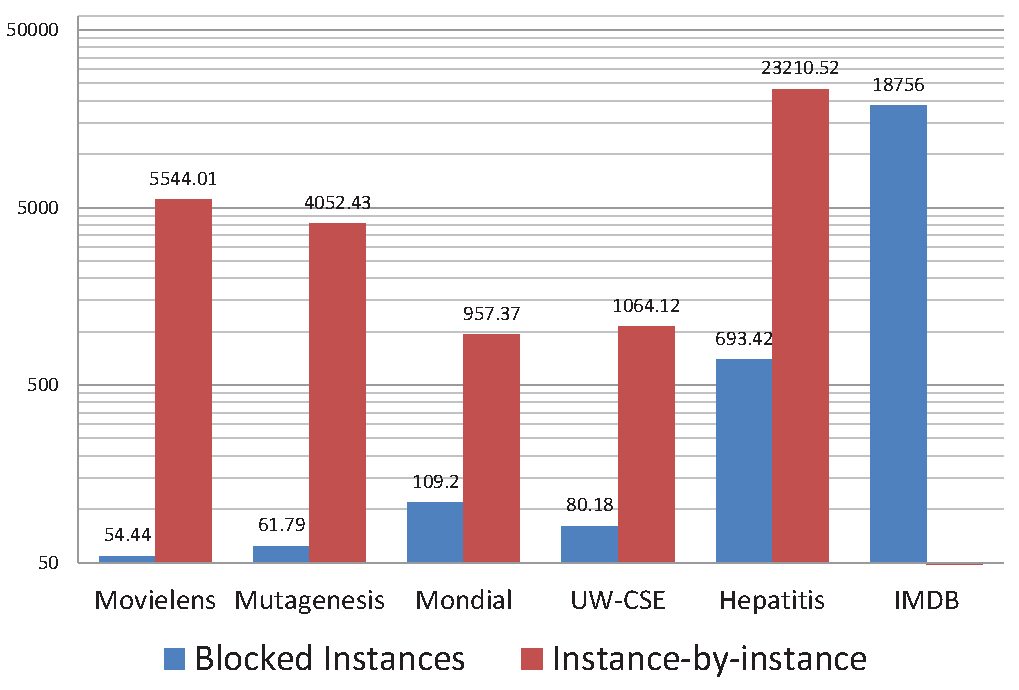
\includegraphics[width=0.5\textwidth]{test-timing.pdf} 
} 
\caption{Test Timing.   
}
 \label{fig:test-timing}
\end{figure}

\section{Other Applications}

In this section we outline how the MRLBase framework can be applied to support other machine learning applications. This discussion is mean to illustrate the potential of MRLBase for other machine learning applications beyond Bayesian network learning.

\subsection{Markov Networks} Markov networks or undirected graphical models have been applied extensively to relational data \cite{taskar,domingos}. An  undirected graphical model defines a log-linear equation for classification. Markov Logic Networks (MLNs) define a widely applied logic-based formalism for specifying the random variables in a Markov network \cite{domingos}. An MLN structure is defined as a set of first-order logic formulas. Typically these formulas are conjunctive queries of the type that define relational contingency tables. 

One option for learning a Markov Logic Network structure is to first learn a Bayesian network structure, then transform the BN structure to an MLN using a standard conversion method (moralization) \cite{MLJ}. This means that the MRLBase method we have described for learning Bayesian networks can be directly applied for learning Markov Logic Networks with RDMBS support. For complex relational schemas, the MRLBase approach to learning MLNs is much more scalable than previous MLN learning methods (scales to millions of records rather than hundreds of thousands). The accuracy of the Bayesian network approach is competive if not greater \cite{}.

An MLN structure can be represented in a database table just like a BN structure. A conjunctive formula is a list $\node_{1} = \value_{1},\ldots,\node_{k} = \value_{k}$. A list of formulas can be represented in a table $\MLN\_\it{Structure}$ with four columns $\it{Index},\it{Variable},\it{Value}$, where $\it{Index}$ stores the index $i$ of a formula, $\it{Variable}$ stores the ID of a relational random variable in formula $i$, and $\it{Value}$ stores the value assigned to the variable in formula $i$. Given a database representation of a BN structure, and the variable domain information in the random variable database, it is straightforward to implement moralization to convert the BN structure table to a corresponding MLN structure table. 

This approach has potential not only for supporting scalable multi-relational learning, but also for probabilistic inference based on a learned model. Database researchers have developed powerful probabilistic inference algorithms that leverage RDBMS capabilities for inference much as MRLBase does for learning \cite{Bayestore,Tuffy}. Such inference algorithms treat statistical objects as first-class citizens in a relational database as MRLBase does. The Tuffy system achieves highly reliable and scalable inference for MLNs with an RDBMS. A future project with great potential is to combine MLN learning by MRLBase with inference by the Tuffy system to produce a single integrated RDBMS package for both learning and inference. 

\subsection{Classification With Aggregate Functions}

A prominent alternative to log-linear models for relational classification is to use aggregate functions \cite{prms,survey,treeliker}. The general idea is to ``flatten'' or ``propositionalize'' the relational structure by summarizing the information about links and linked entities in terms of aggregate features of the target individuals. These aggregate features can be visualized as new columns added to the entity table representing target individuals. Classification can then be performed using any standard single-table classifier (SVM, logistic regression). In our university example, we may compute the average capability score of a student and his or her average grade in courses. This would generate two new features of students that can be used for predicting the intelligence of a student.  


- Classification: log-linear, already discussed.
- aggregate features, like Popescul. Store SQL queries.
- collective matrix factorization, tensor factorization. 
1M parameters. 




\section{Conclusion and Future Work} 
OLAP? Hadoop? Tuffy?
We described different methods for extending relational Bayes net learning to correlations involving links. 
Statistical measures indicate that Bayes net methods succeed in finding relevant correlations. 
There is a trade-off between statistical power and computational feasibility (full table search vs constrained search). 
Hierarchical search often does well on both dimensions, but needs to be extended with a pruning step to eliminate redundant edges.

A key issue for scalability is that most of the learning time is taken up by forming table joins, whose size is the cross product of entity tables. 
These table joins provide the sufficient statistics required in model selection. 
To improve scalability, computing sufficient statistics needs to be feasible for cross product sizes in the millions or more. 
A possible solution may be the virtual join methods that compute sufficient statistics without materializing table joins, such as the Fast M\"obius Transform~\cite{Schulte2012b,Yin2004}.

A valuable direction for future work is to compare learning link correlations with directed and undirected models, such as Markov Logic Networks \cite{Domingos2009}. As we explained in Section~\ref{sec:related}, current relational learners for undirected models do not scale to most of our datasets. One option is to subsample the datasets so that we can compare the statistical power of directed and undirect learning methods
independently of scalability issues. Khosravi {\em et al.} were able to obtain structure learning results for Alchemy~\cite{Khosravi2010}, but did not evaluate the models with respect to link correlations. For the MLN-Boost system, we were able to obtain preliminary results on several benchmark databases  (including Mutagenesis and Hepatitis), by selecting the right subset of target predicates. MLN-Boost is the current state-of-the-art learner for Markov Logic Networks \cite{Khot2011}. The Bayes net models were competitive with the MLN-Boost models on a standard cross-validation measure of predictive accuracy.




%ACKNOWLEDGMENTS are optional
\section{Acknowledgments}

This research was supported by a Discovery grant to Oliver Schulte by the Natural Sciences and Engineering Research Council of Canada. 
Zhensong Qian was supported by a grant from the China Scholarship Council.
We thank the organizers for providing a discussion venue, and the anonymous reviewers for constructive criticism.


% The following two commands are all you need in the
% initial runs of your .tex file to
% produce the bibliography for the citations in your paper.
\bibliographystyle{abbrv}
\bibliography{master} 

 % vldb_sample.bib is the name of the Bibliography in this case
% You must have a proper ".bib" file
%  and remember to run:
% latex bibtex latex latex
% to resolve all references

%\subsection{References}

%%APPENDIX is optional.
%% ****************** APPENDIX **************************************
%% Example of an appendix; typically would start on a new page
%\newpage
%\pagebreak
%
\begin{appendix}
You can use an appendix for optional proofs or details of your evaluation which are not absolutely necessary to the core understanding of your paper. 
\begin{table}[htbp]
  \centering
\resizebox{0.5\textwidth}{!}{
    \begin{tabular}{|r|r|r|r|r|r|}
    \hline
    \multicolumn{2}{|c|}{Table Name} & \multicolumn{4}{c|}{Schema}  \\
    \hline
    \multicolumn{2}{|l|}{AttributeColumns} & \multicolumn{4}{l|}{\begin{tabular}{l}TABLE\_NAME,  COLUMN\_NAME   \end{tabular}}  \\
    \hline
    \multicolumn{2}{|l|}{Domain} & \multicolumn{4}{l|}{\begin{tabular}{l}COLUMN\_NAME, VALUE   \end{tabular}}  \\
    \hline
    \multicolumn{2}{|l|}{Pvariables} & \multicolumn{4}{l|}{\begin{tabular}{l}Pvid,  TABLE\_NAME  \end{tabular}}  \\
    \hline
    \multicolumn{2}{|l|}{1Variables} & \multicolumn{4}{l|}{\begin{tabular}{l}1VarID,  COLUMN\_NAME,  Pvid 
\end{tabular} }  \\
    \hline
    \multicolumn{2}{|l|}{2Variables } & \multicolumn{4}{l|}{\begin{tabular}{ll} 2VarID,  COLUMN\_NAME,  Pvid1,  Pvid2, \\ TABLE\_NAME \end{tabular}}  \\
    \hline
    \multicolumn{2}{|l|}{Relationship} & \multicolumn{4}{l|}{\begin{tabular}{lll}RVarID,  TABLE\_NAME, Pvid1,  Pvid2, \\ COLUMN\_NAME1,  COLUMN\_NAME2  \end{tabular}}  \\
    \hline
    \end{tabular}%
}
  \caption{Schema for Random Variable Database}
  \label{table:rvdb1}%
\end{table}%
\begin{figure}[htbp]
\begin{center}
\resizebox{0.5\textwidth}{!}{
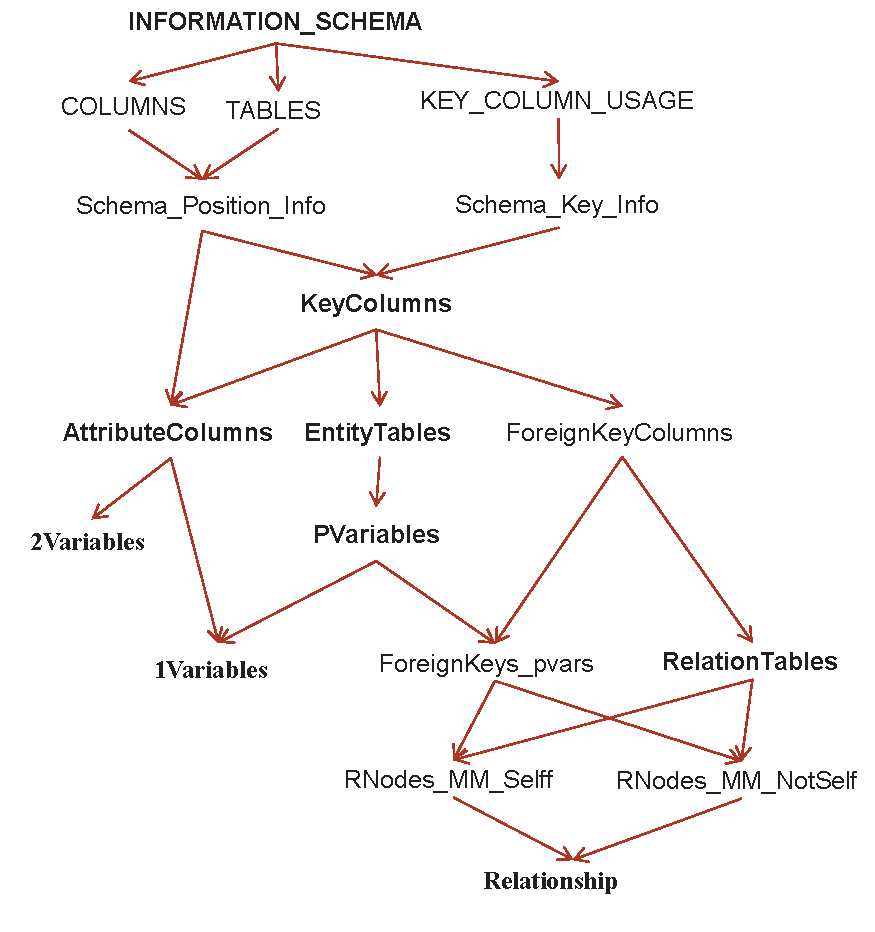
\includegraphics[width=0.5\textwidth]{rv_db.pdf} %move to the appendix
%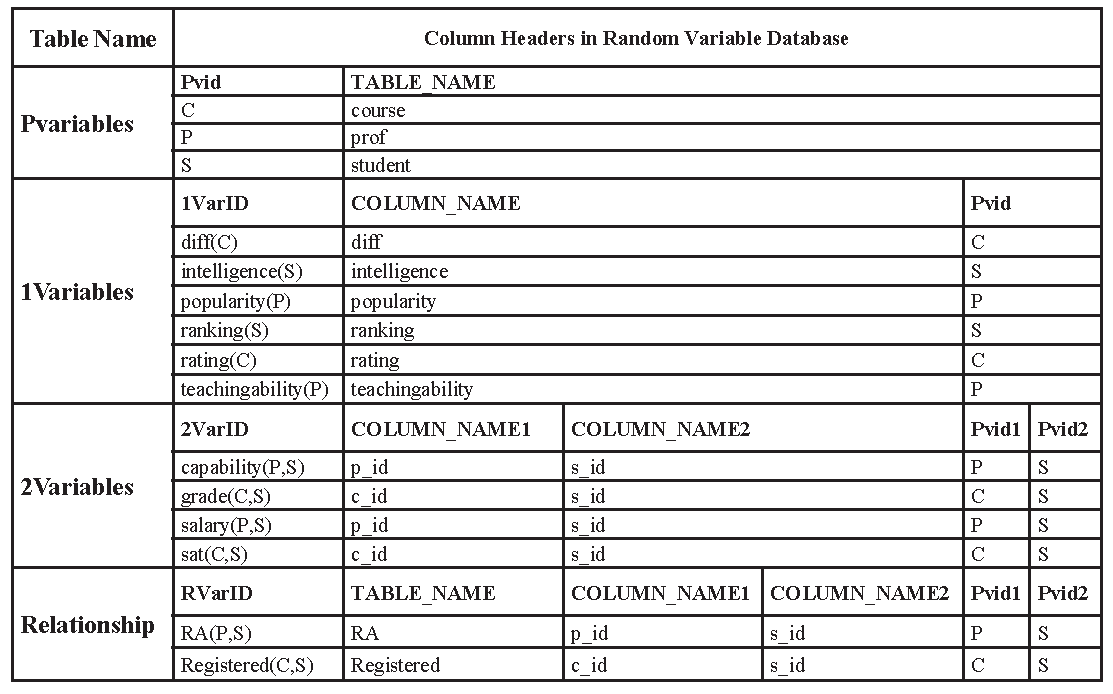
\includegraphics[width=0.5\textwidth]{rv_db_tables.pdf}
}
\caption{Tables  Dependency in the Random Variable Database $\RVD$.
\label{fig:rv_db1}}
\end{center}
\end{figure}

\small
\begin{alltt}
/*AchemaAnalyzer.sql*/
DROP SCHEMA IF EXISTS @database@_AchemaAnalyzer; 
CREATE SCHEMA  @database@_AchemaAnalyzer;

CREATE SCHEMA  if not exists @database@_BN;
CREATE SCHEMA  if not exists @database@_CT;

USE @database@_AchemaAnalyzer;
SET storage_engine=INNODB;

CREATE TABLE Schema_Key_Info AS SELECT TABLE_NAME, COLUMN_NAME,
REFERENCED_TABLE_NAME, REFERENCED_COLUMN_NAME, CONSTRAINT_NAME FROM
INFORMATION_SCHEMA.KEY_COLUMN_USAGE WHERE (KEY_COLUMN_USAGE.TABLE_SCHEMA =
'@database@') ORDER BY TABLE_NAME;

CREATE TABLE Schema_Position_Info AS SELECT COLUMNS.TABLE_NAME,
COLUMNS.COLUMN_NAME,
COLUMNS.ORDINAL_POSITION FROM
INFORMATION_SCHEMA.COLUMNS,
INFORMATION_SCHEMA.TABLES
WHERE
(COLUMNS.TABLE_SCHEMA = '@database@'
    AND TABLES.TABLE_SCHEMA = '@database@'
    AND TABLES.TABLE_NAME = COLUMNS.TABLE_NAME
    AND TABLES.TABLE_TYPE = 'BASE TABLE')
ORDER BY TABLE_NAME;

CREATE TABLE NoPKeys AS SELECT TABLE_NAME FROM
Schema_Key_Info
WHERE
TABLE_NAME NOT IN (SELECT 
        TABLE_NAME
    FROM
        Schema_Key_Info
    WHERE
        CONSTRAINT_NAME LIKE 'PRIMARY');

CREATE table NumEntityColumns AS
SELECT 
    TABLE_NAME, COUNT(DISTINCT COLUMN_NAME) num
FROM
    Schema_Key_Info
WHERE
    CONSTRAINT_NAME LIKE 'PRIMARY'
        OR REFERENCED_COLUMN_NAME IS NOT NULL
GROUP BY TABLE_NAME;

CREATE TABLE TernaryRelations as SELECT TABLE_NAME FROM
NumEntityColumns
WHERE
num > 2;

CREATE TABLE KeyColumns AS SELECT * FROM
(Schema_Key_Info
NATURAL JOIN Schema_Position_Info)
WHERE
TABLE_NAME NOT IN (SELECT 
        TABLE_NAME
    FROM
        NoPKeys)
    AND TABLE_NAME NOT IN (SELECT 
        TABLE_NAME
    FROM
        TernaryRelations);

CREATE TABLE AttributeColumns AS SELECT TABLE_NAME, COLUMN_NAME FROM
Schema_Position_Info
WHERE
(TABLE_NAME , COLUMN_NAME) NOT IN (SELECT 
        TABLE_NAME, COLUMN_NAME
    FROM
        KeyColumns)
    and TABLE_NAME NOT IN (SELECT 
        TABLE_NAME
    FROM
        NoPKeys)
    and TABLE_NAME NOT IN (SELECT 
        TABLE_NAME
    FROM
        TernaryRelations);

ALTER TABLE AttributeColumns ADD PRIMARY KEY (TABLE_NAME,COLUMN_NAME);

CREATE TABLE InputColumns AS SELECT * FROM
KeyColumns
WHERE
CONSTRAINT_NAME = 'PRIMARY'
ORDER BY TABLE_NAME;

CREATE TABLE ForeignKeyColumns AS SELECT * FROM
KeyColumns
WHERE
REFERENCED_COLUMN_NAME IS NOT NULL
ORDER BY TABLE_NAME;

ALTER TABLE ForeignKeyColumns ADD PRIMARY KEY (TABLE_NAME,COLUMN_NAME,REFERENCED_TABLE_NAME);

CREATE TABLE EntityTables AS SELECT distinct TABLE_NAME, COLUMN_NAME FROM
KeyColumns T
WHERE
1 = (SELECT 
        COUNT(COLUMN_NAME)
    FROM
        KeyColumns T2
    WHERE
        T.TABLE_NAME = T2.TABLE_NAME
            AND CONSTRAINT_NAME = 'PRIMARY');

ALTER TABLE EntityTables ADD PRIMARY KEY (TABLE_NAME,COLUMN_NAME);

CREATE TABLE SelfRelationships AS SELECT DISTINCT RTables1.TABLE_NAME AS TABLE_NAME,
RTables1.REFERENCED_TABLE_NAME AS REFERENCED_TABLE_NAME,
RTables1.REFERENCED_COLUMN_NAME AS REFERENCED_COLUMN_NAME FROM
KeyColumns AS RTables1,
KeyColumns AS RTables2
WHERE
(RTables1.TABLE_NAME = RTables2.TABLE_NAME)
    AND (RTables1.REFERENCED_TABLE_NAME = RTables2.REFERENCED_TABLE_NAME)
    AND (RTables1.REFERENCED_COLUMN_NAME = RTables2.REFERENCED_COLUMN_NAME)
    AND (RTables1.ORDINAL_POSITION < RTables2.ORDINAL_POSITION);

ALTER TABLE SelfRelationships ADD PRIMARY KEY (TABLE_NAME);

CREATE TABLE Many_OneRelationships AS SELECT KeyColumns1.TABLE_NAME FROM
KeyColumns AS KeyColumns1,
KeyColumns AS KeyColumns2
WHERE
(KeyColumns1.TABLE_NAME , KeyColumns1.COLUMN_NAME) IN (SELECT 
        TABLE_NAME, COLUMN_NAME
    FROM
        InputColumns)
    AND (KeyColumns2.TABLE_NAME , KeyColumns2.COLUMN_NAME) IN (SELECT 
        TABLE_NAME, COLUMN_NAME
    FROM
        ForeignKeyColumns)
    AND (KeyColumns2.TABLE_NAME , KeyColumns2.COLUMN_NAME) NOT IN (SELECT 
        TABLE_NAME, COLUMN_NAME
    FROM
        InputColumns);

CREATE TABLE PVariables AS SELECT CONCAT(EntityTables.TABLE_NAME, '0') AS Pvid,
EntityTables.TABLE_NAME,
0 AS index_number FROM
EntityTables 
UNION 
SELECT 
CONCAT(EntityTables.TABLE_NAME, '1') AS Pvid,
EntityTables.TABLE_NAME,
1 AS index_number
FROM
EntityTables,
SelfRelationships
WHERE
EntityTables.TABLE_NAME = SelfRelationships.REFERENCED_TABLE_NAME
    AND EntityTables.COLUMN_NAME = SelfRelationships.REFERENCED_COLUMN_NAME ;

ALTER TABLE PVariables ADD PRIMARY KEY (Pvid);

CREATE TABLE RelationTables AS SELECT DISTINCT ForeignKeyColumns.TABLE_NAME,
ForeignKeyColumns.TABLE_NAME IN (SELECT 
        TABLE_NAME
    FROM
        SelfRelationships) AS SelfRelationship,
ForeignKeyColumns.TABLE_NAME IN (SELECT 
        TABLE_NAME
    FROM
        Many_OneRelationships) AS Many_OneRelationship FROM
ForeignKeyColumns;

ALTER TABLE RelationTables ADD PRIMARY KEY (TABLE_NAME);

CREATE TABLE 1Variables AS SELECT CONCAT('`', COLUMN_NAME, '(', Pvid, ')', '`') AS 1VarID,
COLUMN_NAME,
Pvid,
index_number = 0 AS main FROM
PVariables
    NATURAL JOIN
AttributeColumns;

ALTER TABLE 1Variables ADD PRIMARY KEY (1VarID);
ALTER TABLE 1Variables ADD UNIQUE(Pvid,COLUMN_NAME);

CREATE TABLE ForeignKeys_pvars AS SELECT ForeignKeyColumns.TABLE_NAME,
ForeignKeyColumns.REFERENCED_TABLE_NAME,
ForeignKeyColumns.COLUMN_NAME,
Pvid,
index_number,
ORDINAL_POSITION AS ARGUMENT_POSITION FROM
ForeignKeyColumns,
PVariables
WHERE
PVariables.TABLE_NAME = REFERENCED_TABLE_NAME;

ALTER TABLE ForeignKeys_pvars ADD PRIMARY KEY (TABLE_NAME,Pvid,ARGUMENT_POSITION);

CREATE table Relationship_MM_NotSelf AS
SELECT 
    CONCAT('`',
            ForeignKeys_pvars1.TABLE_NAME,
            '(',
            ForeignKeys_pvars1.Pvid,
            ',',
            ForeignKeys_pvars2.Pvid,
            ')',
            '`') AS orig_RVarID,
    ForeignKeys_pvars1.TABLE_NAME,
    ForeignKeys_pvars1.Pvid AS Pvid1,
    ForeignKeys_pvars2.Pvid AS Pvid2,
    ForeignKeys_pvars1.COLUMN_NAME AS COLUMN_NAME1,
    ForeignKeys_pvars2.COLUMN_NAME AS COLUMN_NAME2,
    (ForeignKeys_pvars1.index_number = 0
        AND ForeignKeys_pvars2.index_number = 0) AS main
FROM
    ForeignKeys_pvars AS ForeignKeys_pvars1,
    ForeignKeys_pvars AS ForeignKeys_pvars2,
    RelationTables
WHERE
    ForeignKeys_pvars1.TABLE_NAME = ForeignKeys_pvars2.TABLE_NAME
        AND RelationTables.TABLE_NAME = ForeignKeys_pvars1.TABLE_NAME
        AND ForeignKeys_pvars1.ARGUMENT_POSITION < ForeignKeys_pvars2.ARGUMENT_POSITION
        AND RelationTables.SelfRelationship = 0
        AND RelationTables.Many_OneRelationship = 0;

CREATE table Relationship_MM_Self AS
SELECT 
    CONCAT('`',
            ForeignKeys_pvars1.TABLE_NAME,
            '(',
            ForeignKeys_pvars1.Pvid,
            ',',
            ForeignKeys_pvars2.Pvid,
            ')',
            '`') AS orig_RVarID,
    ForeignKeys_pvars1.TABLE_NAME,
    ForeignKeys_pvars1.Pvid AS Pvid1,
    ForeignKeys_pvars2.Pvid AS Pvid2,
    ForeignKeys_pvars1.COLUMN_NAME AS COLUMN_NAME1,
    ForeignKeys_pvars2.COLUMN_NAME AS COLUMN_NAME2,
    (ForeignKeys_pvars1.index_number = 0
        AND ForeignKeys_pvars2.index_number = 1) AS main
FROM
    ForeignKeys_pvars AS ForeignKeys_pvars1,
    ForeignKeys_pvars AS ForeignKeys_pvars2,
    RelationTables
WHERE
    ForeignKeys_pvars1.TABLE_NAME = ForeignKeys_pvars2.TABLE_NAME
        AND RelationTables.TABLE_NAME = ForeignKeys_pvars1.TABLE_NAME
        AND ForeignKeys_pvars1.ARGUMENT_POSITION < ForeignKeys_pvars2.ARGUMENT_POSITION
        AND ForeignKeys_pvars1.index_number < ForeignKeys_pvars2.index_number
        AND RelationTables.SelfRelationship = 1
        AND RelationTables.Many_OneRelationship = 0;

CREATE table Relationship_MO_NotSelf AS
SELECT 
    CONCAT('`',
            ForeignKeys_pvars.REFERENCED_TABLE_NAME,
            '(',
            PVariables.Pvid,
            ')=',
            ForeignKeys_pvars.Pvid,
            '`') AS orig_RVarID,
    ForeignKeys_pvars.TABLE_NAME,
    PVariables.Pvid AS Pvid1,
    ForeignKeys_pvars.Pvid AS Pvid2,
    KeyColumns.COLUMN_NAME AS COLUMN_NAME1,
    ForeignKeys_pvars.COLUMN_NAME AS COLUMN_NAME2,
    (PVariables.index_number = 0
        AND ForeignKeys_pvars.index_number = 0) AS main
FROM
    ForeignKeys_pvars,
    RelationTables,
    KeyColumns,
    PVariables
WHERE
    RelationTables.TABLE_NAME = ForeignKeys_pvars.TABLE_NAME
        AND RelationTables.TABLE_NAME = PVariables.TABLE_NAME
        AND RelationTables.TABLE_NAME = KeyColumns.TABLE_NAME
        AND RelationTables.SelfRelationship = 0
        AND RelationTables.Many_OneRelationship = 1;

CREATE table Relationship_MO_Self AS
SELECT 
    CONCAT('`',
            ForeignKeys_pvars.REFERENCED_TABLE_NAME,
            '(',
            PVariables.Pvid,
            ')=',
            ForeignKeys_pvars.Pvid,
            '`') AS orig_RVarID,
    ForeignKeys_pvars.TABLE_NAME,
    PVariables.Pvid AS Pvid1,
    ForeignKeys_pvars.Pvid AS Pvid2,
    KeyColumns.COLUMN_NAME AS COLUMN_NAME1,
    ForeignKeys_pvars.COLUMN_NAME AS COLUMN_NAME2,
    (PVariables.index_number = 0
        AND ForeignKeys_pvars.index_number = 1) AS main
FROM
    ForeignKeys_pvars,
    RelationTables,
    KeyColumns,
    PVariables
WHERE
    RelationTables.TABLE_NAME = ForeignKeys_pvars.TABLE_NAME
        AND RelationTables.TABLE_NAME = PVariables.TABLE_NAME
        AND RelationTables.TABLE_NAME = KeyColumns.TABLE_NAME
        AND PVariables.index_number < ForeignKeys_pvars.index_number
        AND RelationTables.SelfRelationship = 1
        AND RelationTables.Many_OneRelationship = 1;

CREATE TABLE Relationship AS SELECT * FROM  
Relationship_MM_NotSelf    
UNION SELECT            
*                   
FROM
Relationship_MM_Self 
UNION SELECT 
*
FROM
Relationship_MO_NotSelf 
UNION SELECT 
*
FROM
Relationship_MO_Self;

ALTER TABLE Relationship ADD PRIMARY KEY (orig_RVarID);
ALTER TABLE `Relationship` ADD COLUMN `RVarID` VARCHAR(10) NULL , ADD UNIQUE INDEX `RVarID_UNIQUE` (`RVarID` ASC) ; 


CREATE TABLE 2Variables AS SELECT CONCAT('`',
        COLUMN_NAME,
        '(',
        Pvid1,
        ',',
        Pvid2,
        ')',
        '`') AS 2VarID,
COLUMN_NAME,
Pvid1,
Pvid2,
TABLE_NAME,
main FROM
Relationship
    NATURAL JOIN
AttributeColumns;

ALTER TABLE 2Variables ADD PRIMARY KEY (2VarID);</p>\end{alltt}

%\section{Final Thoughts on Good Layout}
%Please use readable font sizes in the figures and graphs. Avoid tempering with the correct border values, and the spacing (and format) of both text and captions of the PVLDB format (e.g. captions are bold).
%
%At the end, please check for an overall pleasant layout, e.g. by ensuring a readable and logical positioning of any floating figures and tables. Please also check for any line overflows, which are only allowed in extraordinary circumstances (such as wide formulas or URLs where a line wrap would be counterintuitive).
%
%Use the \texttt{balance} package together with a \texttt{\char'134 balance} command at the end of your document to ensure that the last page has balanced (i.e. same length) columns.

\end{appendix}



\end{document}


%The databases are fairly complex, so the experiments are computationally demanding, especially the Alchemy inference component, which needs to be applied to all groundings of all descriptive attributes to compute average predictive performance. The databases and their main characteristics are as follows. 
% and on-line sources such as \cite{bib:jbnsite}.
%In this paper we report the average result over all subdatabases in this paper and leave the evaluation of how models should evolve based on the size of data to an extension of the work in a journal paper. 
%
%\textbf{to do}
%Also, we may emphasize the difference of such datasets in terms of self-relationships and same type relationships.
%
%\noindent\textbf{University Database.} We manually created a small dataset, based on the schema given in Figure~\ref{fig:university-schema}.% omitting the $\it{Teaches}$ relationship for simplicity. 
%The dataset is small and is used as a testbed for the correctness of our algorithms.
%
%\noindent\textbf{MovieLens Database } 
%%A dataset from the UC Irvine machine learning repository. The data are organized in 3 tables (2 entity tables, 1 relationship table, and 7 descriptive attributes). 
%
%This is a standard dataset from the UC Irvine machine learning repository.  \textbf{really? I can NOT find it online.}
%%user:6039; Movie: 3883; rating: 1000129
%%age, 7 bins based on the original MovieLens design
%
%% \cite{Schulte2012}.
%%The schema for the dataset is shown in Table \ref{}.
%It contains two tables representing entity sets: User with 6,039 tuples and Item (Movies) with 3,883 tuples.
%The User table has 2 descriptive attributes, $\age$ and $\it{gender}$. We discretized the attribute $\age$ into three equal-frequency bins. 
%The table Item represents information about the movies. 
%%It has 17 Boolean attributes that indicate the genres of a given movie. 
%There is one relationship table Rated corresponding to a Boolean predicate. 
%The Rated contains Rating as descriptive attribute; 1,000,129 ratings are recorded.  
%We performed a preliminary data analysis following \cite{Schulte2012}.
%%and omitted genres that have only weak correlations with the rating or user attributes, leaving a total of three genres (Drama, Horror, Action).
%
%%
%%The full dataset contains 170,143 ground atoms and is too big for Alchemy to perform learning. We made small subsamples to make the experiments feasible. Subsampling 100 Users and 100 Items transforms to an Alchemy input file with 3,485 ground atoms. Structure learning with Alchemy takes around 30 min.
%%Subsampling 300 Users and 300 Items transforms to an Alchemy input file with 27,134 ground atoms. Structure learning with Alchemy takes about 2 days to run.
%%The full table with 100,000 ratings exceeded the memory limits of Tetrad, so we randomly picked 40\% of the ratings of the relationship table as input data.
%
%\noindent\textbf{Mutagenesis Database.}  This dataset is widely used in Inductive Logic Programming research \cite{Srinivasan1996}. %It contains 4 tables total to 15218 tuples. 
%We used a previous discretization \cite{Schulte2012}.
%Mutagenesis has two entity tables, Atom with 3 descriptive attributes, and Mole (decribing molecules), with 5 descriptive attributes. 
%%including two attributes that are discretized into ten values each (logp and lumo).
%There are two relationship tables, MoleAtom, indicating which atoms are parts of which molecules, and Bond, which relates two atoms and has 1 descriptive attribute. 
%%The full dataset, with 35,973 ground atoms, crashed Alchemy with both structure  and parameter learning. A subsample with 5,017 ground atoms did not terminate for structure learning, but weight learning was feasible. The computational difficulties of Alchemy compared to the MovieLens dataset are  due to the high number of descriptive attributes.
%%%another subsample with
%%Representing a relationship between entities from the same table in a parametrized Bayes net requires using two or more variables associated with the same population (e.g., $\it{Bond}(\A_{1},\A_{2}))$.
%%(Techreport 2009) describes a straightforward extension of Algorithm~\ref{alg:structure} for this case, which we applied to the Mutagenesis dataset.\footnote{Reference omitted for blind review.}
%%We also tested our method on the Financial dataset with similar results, but omit a discussion due to space constraints.
%
%\noindent\textbf{Financial} 
%This dataset stores the loan information about the clients at the associated banks.
%And it's a modified version of the financial dataset from the discovery challenge that was organized at PKDD'99. We adapted the database design to fit the ER model by following the
%modification from CrossMine~\cite{Yin2004} and Graph-NB~\cite{han2009}.
%The data are organized in 7 tables (4 entity tables, 3 relationship tables with 15 descriptive attributes in total).
%
%
%\noindent\textbf{Hepatitis Database.} This data is a modified version of the PKDD02 Discovery Challenge database \cite{Frank2007}. %, which includes removing tests with null values. 
%The database contains information on laboratory examinations of 771 hepatitis B- and C-infected patients, taken between 1982 and 2001. The data are organized in 7 tables (4 entity tables,  3 relationship tables) with 16 descriptive attributes. They contain basic information about the patients, results of biopsy, information on interferon therapy, results of out-hospital examinations, and results of in-hospital examinations. 
%
%\noindent\textbf{IMDB Database.} %, combination?.}
%This is the most challenge dataset in terms of nubmer of total tuples and ER-Digram complexity. %attributes.
%Basically we make a combination of the MovieLens 1M dataset which is a commonly-used rating dataset\footnote{www.grouplens.org}  and the Internet Movie Database (IMDB)\footnote{www.imdb.com, July 2013}.
%We performed a very {\em similar preliminary data processing} with MovieLens dataset. \cite{Peralta2007}
%Two more entity tables representing actors and directors were introduced, and we added more related information as descriptive attributes about the movies from IMDB. 
%In spite of the rating table, we added another two relationship tables. One is to store who directed the movie with genre information, and the other to store which actors participated in which movies.
%So in total, there are four entity tables, three relationship tables.% with more than 1.3M tuples.
%
%%And also includes 3 relationship tables to represent the 5 star rating score given per movie, which actors are involved in given movie and who directed that movie. 
%%4 entity tables : actors (gender 2, quality 6: 98690 ),directors(quality 6,avg\_revenue 5:2201),movies(year 4,country 4,runningtime 4:3832),users(age 7,gender 2,occuption 5 :6039)
%%and 3 relation tables: u2base(rating 5: 996159), movies2actors(cast\_num 4:138349), movies2directos(genre 9:4141)
%
%
%
%\noindent\textbf{Mondial Database.} A geography database, featuring
%one self-relationship, $\it{Borders}$, that indicates which countries border each other. 
%This dataset contains data from multiple geographical web data sources. 
%We follow the modification of She\cite{wangMondial}, and use a subset of the tables and disretized features: 2 entity tables, $\it{Country},\it{Economy}$. 
%The descriptive attributes of Country are continent, government, percentage, majority religion, population size. The descriptive attributes of Economy are inflation, gdp, service, agriculture, industry. 
%Another relationship table is  Economy\_Country specifying which country has what type of economy. %A self-relationship table Borders relates two countries.
%  %$\it{Country},\it{Continent},\it{Economy},\it{Government}$, where the latter three are related to Country by many-one relationships, and one relationship table $\it{Borders}$ that relates two countries. Our dataset includes a self-relationship table Borders that relates two countries.
%
%
%\noindent\textbf{UW-CSE Database.}
%This dataset lists facts about the Department of Computer Science and Engineering at the University of Washington. There're two entity  tables (i.e., $Person$, $Course$) and two relationship tables (i.e. $AdvisedBy$, $TaughtBy$).
%And these two tables both involve a self-relationship relating to two persons \cite{Domingos2007}. 
%%The total number of ground atoms is 4,106,841. The database contained a total of 3380 ground atoms. 
%
%
%\begin{table}[btp] \centering
%%\scalebox{0.7in}{
%\resizebox{0.5\textwidth}{!}{
%\begin{tabular}[c]
%{|l|c|c|c|r|r|}\hline
% \textbf{Dataset} & \textbf{\#Relations} & \textbf{Self} &
% \textbf{SameType}& \textbf{\#Tuples} & \textbf{\#Attribute}  \\\hline
%% \textbf{Dataset} & \textbf{Relationships} & \textbf{\begin{tabular}[l] {ll} Self \\Relationships \end {tabular}} &
%% \textbf{\begin{tabular}[l] {ll} Same Type\\ Relationships \end {tabular}}& \textbf{\#Tuples} & \textbf{\begin{tabular}[l] {ll} \#Attribute  \\Columns \end{tabular}}  \\\hline
%    University&2 & N & N & 171 & 12\\\hline
%    Movielens &1 & N & N & 1,010,051 & 7\\\hline
%%    Movielens(0.1M) &1 & N & N &  83,402 & 7\\\hline
%    Mutagenesis &2 & N & \textbf{Y} & 14,540 & 11\\\hline
%    Financial &3 & N & N &  225,932& 15\\\hline
%   Hepatitis &3 & N & N &12,927  & 19\\\hline
%   IMDB &3 & N &N &1,354,134  & 17\\\hline
%    Mondial &2 & \textbf{Y} & N &  870& 18\\\hline
%    UW-CSE &2 & \textbf{Y} & N & 712 & 14\\\hline
%   
%\end{tabular}
%}
% % end scalebox
%\caption{Real datasets characteristics, including size of datasets in total number of table tuples. 
% \# Attribute should not count the $Rnodes$ ? Here Self means self relationship, and type means same type relationship or not.
% \label{table:datasetsize}}
%\end{table}
%
%
%\subsection{Methods Compared}
%%\paragraph{Methods Compared}
%
%We compared the following methods.
%
%\begin{description}
%\item[Bayes Base Hierarchical Search (B.B.H.) ] The new method that has the potential to find link correlations (Algorithm~\ref{alg:fmt} with the $\ct$-tables instead of natural join tables).
%\item[Flat Search]  Applies the single-table Bayes net learner to the biggest $\ct$-table.
%\item[Complete Graph] fully connected DAG.
%\item[Disconnected Graph] all nodes are disconnected.
%
%\end{description}
%
%To implement Flat Search and the LAJ+ algorithm efficiently, we apply the Fast M\"obius Transform to compute tables of sufficient statistics that involve negated relationships. We discuss the details further in Section~\ref{sec:mobius}.
%
%\subsection{Learning Times: SQL Join Time?}
%
% Table~\ref{table:cttimes} shows the data preprocessing time that the different methods require for table joins. This is the same for all methods, namely the cost of computing the full join table using the fast M\"obius transform described in Section~\ref{sec:mobius}. 
%\begin{table} \centering
%%\scalebox{0.7in}{
%\resizebox{0.5\textwidth}{!}{
%\begin{tabular}
%{|l|r|r|r|r|}\hline 
% \textbf{Dataset} & \textbf{Building Time} & \textbf{Sum(counts)}  & \textbf{\#Tuples} & \textbf{Compress Ratio} \\\hline
%University&1.68/0.05 & 2,280 & 351 &6.5 \\\hline
%Movielens &2.70/703.99 &23,449,437 &252 &93,053.32\\\hline
%%Movielens(0.1M) &0.62 & 1,582,762 &239 &6,622.44 \\\hline
%Mutagenesis &1.67/1096.00 & 905,205 &1,631 &555.00  \\\hline
%Financial &  1421.87/12592.41(N.T.) &149,046,585,349,303 &3,013,011 &49,467,653.90   \\\hline
%Hepatitis &3536.76/6075.39 &17,846,976,000 & 12,374,892 &1,442.19 \\\hline
%IMDB &7467.85/17526.86(N.T.) &5,030,412,758,502,710&15,538,430 & 323,740,092.05 \\\hline
%Mondial &1112.84/132.13&4,655,957&1,746,870&2.67  \\\hline
%UW-CSE &3.84/350.30& 10,201,488&2,828 & 3,607.32\\\hline
%
%\end{tabular}
%}
% % end scalebox
%\caption{Contengency Table (C.T.) Description : Building Time  in seconds. vs Full Relation Table SQL join time? %The Learn-and-Join methods do the same 
% \label{table:cttimes}}
%\end{table}
%
%
%[fill in discussion] 
%
%
%Table~\ref{table:runtimes}
% provides the model search time for each of the link analysis methods. 
%%This does not include the time for computing table joins since this is essentially the same for all methods (the cost of the full join table). 
%On the smaller and simpler datasets, all search strategies are fast, 
%but on the medium-size and more complex datasets (Hepatitis, MovieLens), hierarchical search is much faster due to its use of constraints.
%%Adding prior knowledge as constraints could speed the structure learning substantially.
%%The reason for w LAJ+ starts with the previous LAJ method as the first phase. The edges among attributes that are discovered in the first phase are treated as fixed background knowledge in the second phase. 
%
%
%\begin{table} \centering
%%\scalebox{0.7in}{
%\resizebox{0.5\textwidth}{!}{
%\begin{tabular}[c]
%{|l|r|r|r|r|r|}\hline
% \textbf{Dataset}  & \textbf{BBH} & \textbf{Flat} & \textbf{Compl.} & \textbf{Discon.}\\\hline
%University&1.523&1.486& 0.186 &0.135 \\\hline
%Movielens & 1.528&0.968& 0.101&0.066 \\\hline
%%Movielens(0.1M) &1.178& 0.986& 0.083&0.065 \\\hline
%Mutagenesis & 1.780&1.869& 0.115&0.096 \\\hline
%Financial  &96.308& 1,241.077& 0.203&0.080 \\\hline
%Hepatitis   & 416.704& N.T.& 0.272&0.134 \\\hline
%IMDB   & 551.643 & N.T.&0.286 &0.220 \\\hline
%Mondial & 190.162&1,289.534&0.280 &0.093 \\\hline
%UW-CSE & 2.896&2.367&0.181 &0.100 \\\hline
%\end{tabular}
%}
% % end scalebox
%\caption{Model Structure Learning Time  in seconds.
%% \textbf{Zhensong: may show some realy SQL queries?}
% \label{table:runtimes}}
%\end{table}
%
%
%
%%\paragraph{Performance Metrics }
%\subsection{Performance Metrics }
%
%\textbf{Pseudo Relation Model Selection Scores  \cite{Schulte2011} ?}, advantages \cite{Schulte2013} ?
%
% We report learning time, log-likelihood, Bayes Information Criterion (BIC), and the Akaike Information Criterion (AIC). BIC and AIC are standard scores for Bayes nets \cite{Chickering2003}, defined as follows. We write 
%$$L(\hat{G},\d)$$ for the log-likelihood score,
%where $\hat{G}$ is the BN $\G$ with its parameters instantiated to be the maximum likelihood estimates given the dataset $\d$, and the quantity $L(\hat{G},\d)$ is the log-likelihood of $\hat{G}$ on $\d$. 
%
%The BIC score is defined as follows \cite{Chickering2003,Schulte2011}
%
%$$\mathit{BIC}(\G,\d) = L(\hat{G},\d) - \mathit{par}(\G)/2 \times ln(m)$$
%
%where the data table size is denoted by $m$, and $\mathit{par}(\G)$ is the number of free parameters in the structure $\G$. The AIC score is given by 
%
%$$\mathit{AIC}(\G,\d) = L(\hat{G},\d) - \mathit{par}(\G). $$
%
% AIC is asympotically equivalent to selection by cross-validation, so we may view it as a closed-form approximation to cross-validation,  which is computationally demanding for relational datasets. 
%
%
%
%
%
%%\section{Empirical Evaluation: Statistical Scores}
%
%
%
%
%\begin{table}[hbtp] 
%\begin{center}
%\resizebox{0.5 \textwidth}{!}{
%\begin{tabular}{|l|r|r|r|r| }
%		\hline \textbf{University} &{Pseudo\_BIC}& {Pseudo\_AIC} &{Norm\_log-likelihood} &{\# Para.}\\
%			\hline BBH &-554.01 & -99.50 & -5.50& 94\\
%			\hline Flat  & -3731.88 & -668.20 & -5.20& 663\\
%			 \hline Complete &-386566.28  & -50000.10& -5.10& 49995 \\
%		        \hline Disconnected &-121.44 &-31.89 &-8.89 &23 \\
%			\hline
%		\end{tabular}
%}
%\end{center}
%
%\begin{center}
%\resizebox{0.5 \textwidth}{!}{
%\begin{tabular}{|l|r|r|r|r| }
%\hline \textbf{Movielens(1M) } &{Pseudo\_BIC}& {Pseudo\_AIC} &{Norm\_log-likelihood} &{\# Para.}\\
%
%			\hline BBH &-4927.84& -295.44& -3.44&292\\
%			\hline Flat &-5168.08&-315.44 &-3.44& 312\\
%		      \hline Complete &-11461.86  &-678.44 &-3.44 &675 \\
%		        \hline Disconnected &-179.20 &-19.31 &-4.31 &15 \\
%			
%			\hline
%		\end{tabular}
%}
%\end{center}
%
%%
%%\begin{center}
%%\resizebox{0.5 \textwidth}{!}{
%%\begin{tabular}{|l|r|r|r|r| }
%%		\hline \textbf{Movielens(0.1M) } &{Pseudo\_BIC}& {Pseudo\_AIC} &{Norm\_log-likelihood} &{\# Para.}\\
%%			\hline BBH &-1198.42&-87.10& -3.10&84\\
%%			\hline Flat &-1691.20&-123.10 &-3.10& 120\\
%%			 \hline Complete &-4160.11  &-294.09 &-3.09 &291 \\
%%		        \hline Disconnected &-120.88 &-14.34 & -3.34&11 \\
%%			
%%			\hline
%%		\end{tabular}
%%}
%%\end{center}
%
%\begin{center}
%\resizebox{0.5 \textwidth}{!}{
%\begin{tabular}{|l|r|r|r|r| }
%		\hline \textbf{Mutagenesis  } &{Pseudo\_BIC}& {Pseudo\_AIC} &{Norm\_log-likelihood} &{\# Para.}\\
%			\hline BBH &-9083.88 &-726.96 &-5.96& 721\\
%			\hline Flat & -9224.25 & -1120.59& -5.59& 1115\\
%			 \hline Complete &-5806905.08  &-423374.59 &-5.59 &423369 \\
%		        \hline Disconnected &-292.7 &-43.91 &-7.91 &36 \\
%			\hline
%		\end{tabular}
%}
%\end{center}
%
%\begin{center}
%\resizebox{0.5 \textwidth}{!}{
%\begin{tabular}{|l|r|r|r|r| }
%		\hline \textbf{Financial  } &{Pseudo\_BIC}& {Pseudo\_AIC}&{Norm\_log-likelihood} &{\# Para.}\\
%			\hline BBH &-68562.16 &-2443.74 &-10.74& 2433\\
%			\hline Flat &-188908818.94 &-7206670.64 & -10.66& 7206660\\
%			 \hline Complete &-12218648361.31  &-374400009.12 & -10.67&374399999 \\
%		        \hline Disconnected &-469.21 &-61.79 &-12.79 & 49\\
%			\hline
%		\end{tabular}
%}
%\end{center}
%
%\begin{center}
%\resizebox{0.5 \textwidth}{!}{
%\begin{tabular}{|l|r|r|r|r| }
%		\hline \textbf{Hepatitis  } &{Pseudo\_BIC}& {Pseudo\_AIC} &{Norm\_log-likelihood} &{\# Para.}\\
%			\hline BBH &-10364.93 & -585.58& -16.58& 569\\
%			\hline Flat &N.T. & &  & \\
%			 \hline Complete & N.T.  & & & \\
%		        \hline Disconnected &-473.81 &-76.30 &-18.30 &58 \\
%			\hline
%		\end{tabular}
%}
%\end{center}
%
%
%\begin{center}
%\resizebox{0.5 \textwidth}{!}{
%\begin{tabular}{|l|r|r|r|r| }
%		\hline \textbf{IMDB  } &{Pseudo\_BIC}& {Pseudo\_AIC}&{Norm\_log-likelihood} &{\# Para.}\\
%			\hline BBH &-2072673.77 & -60070.39&-11.39&60059\\
%			\hline Flat & N.T.&  &  &  \\
%			 \hline Complete &N.T.  & & & \\
%		        \hline Disconnected &-647.90 &-66.01 &-12.01 &54 \\
%			\hline
%		\end{tabular}
%}
%\end{center}
%
%\begin{center}
%\resizebox{0.5 \textwidth}{!}{
%\begin{tabular}{|l|r|r|r|r| }
%		\hline \textbf{Mondial  } &{Pseudo\_BIC}& {Pseudo\_AIC} &{Norm\_log-likelihood} &{\# Para.}\\
%			\hline BBH &-3980.41&-357.20&-18.20& 339\\
%			\hline Flat &-8886625.98 &-865255.07 &-14.07  &865241 \\
%			 \hline Complete &N.T.  & & & \\
%		        \hline Disconnected &-336.50 &-74.98 &-19.98 &55 \\
%			\hline
%		\end{tabular}
%}
%\end{center}
%
%\begin{center}
%\resizebox{0.5 \textwidth}{!}{
%\begin{tabular}{|l|r|r|r|r| }
%		\hline \textbf{UW-CSE  } &{Pseudo\_BIC}& {Pseudo\_AIC} &{Norm\_log-likelihood} &{\# Para.}\\
%			\hline BBH & -3187.86& -248.1 & -8.10 & 240\\
%			\hline Flat &-42038.65& -3939.01 & -6.01& 3933 \\
%			 \hline Complete &-356947710.61  &-22118404.95 &-6.02 &22118399 \\
%		        \hline Disconnected &-287.63 &-55.24 &-10.24 &45 \\
%			\hline
%		\end{tabular}
%}
%\end{center}
%\caption{Statistical Performance of different Searching Algorithms by dataset.}
%\textbf{Zhensong: paramete learning  not terminated, mysql, may show some real SQL queries in the appendix?}
%\label{table:result_scores}
%\end{table}
%
%As expected, adding edges between link nodes improves the statistical data fit: 
%the link analysis methods LAJ+ and Flat perform better than the learn-and-join baseline in terms of log-likelihood on all datasets shown in table~\ref{table:result_scores}, except for MovieLens where the Flat search has a lower likelihood. On the small synthetic dataset University, flat search appears to overfit whereas the hierarchical search methods are very close. On the medium-sized dataset MovieLens, which has a simple structure, all three methods score similarly. Hierarchical search finds no new edges involving the single link indicator node (i.e., LAJ and LAJ+ return the same model). 
%
%The most complex dataset, Hepatitis, is a challenge for flat search, which seems to overfit severely with a huge number of parameters that result in a model selection score that is an order of magnitude worse than for hierarchical search. Because of the complex structure of the Hepatitis schema, the hierarchy constraints appear to be effective in combating overfitting.
%
%%
%%\begin{figure*}[htbp] %  figure placement: here, top, bottom, or page
%%   \centering
%%
%%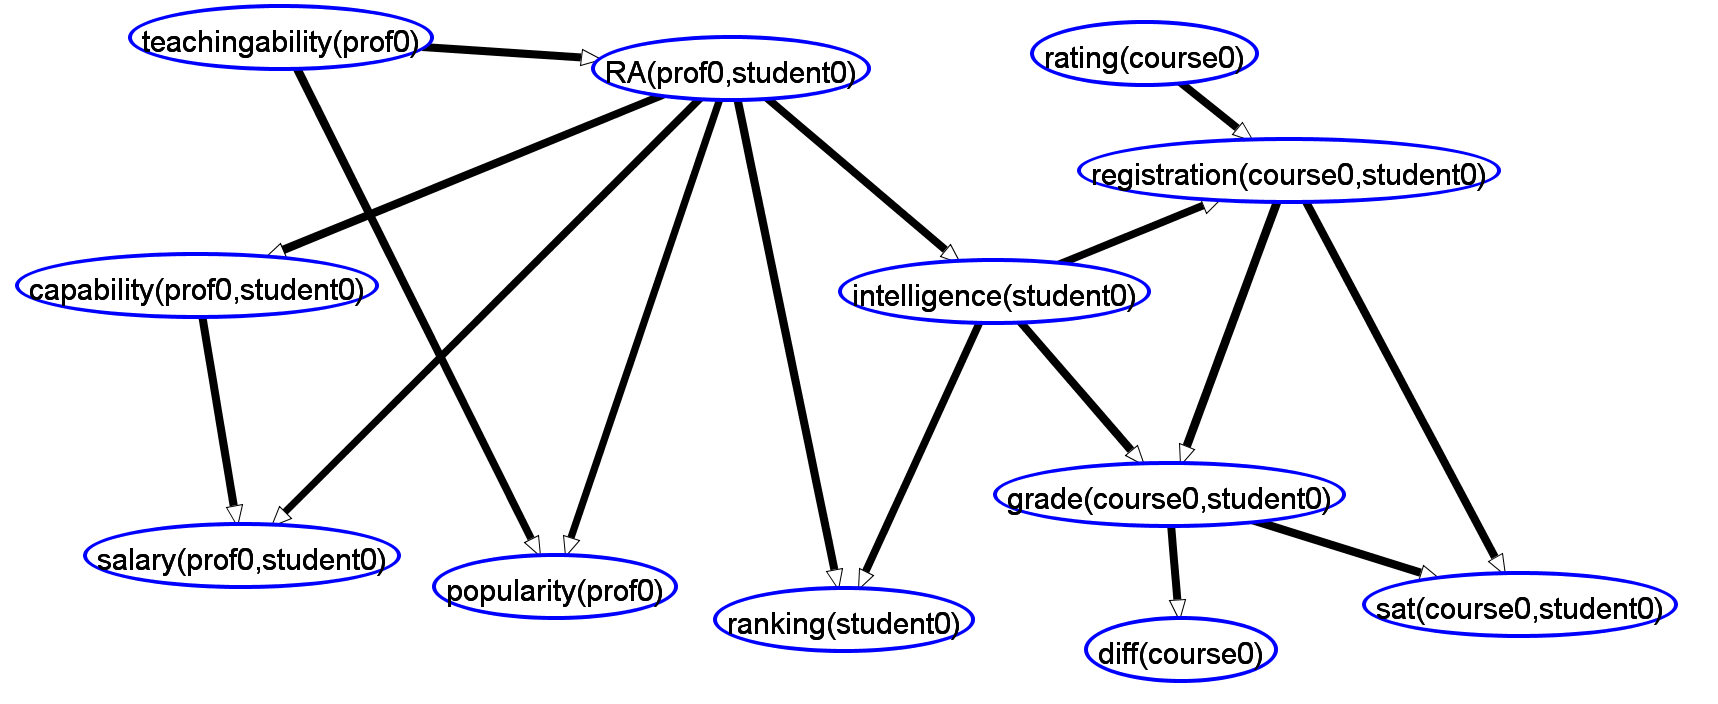
\includegraphics[width=7in,height=0.3\textheight]{unielwin.png}
%%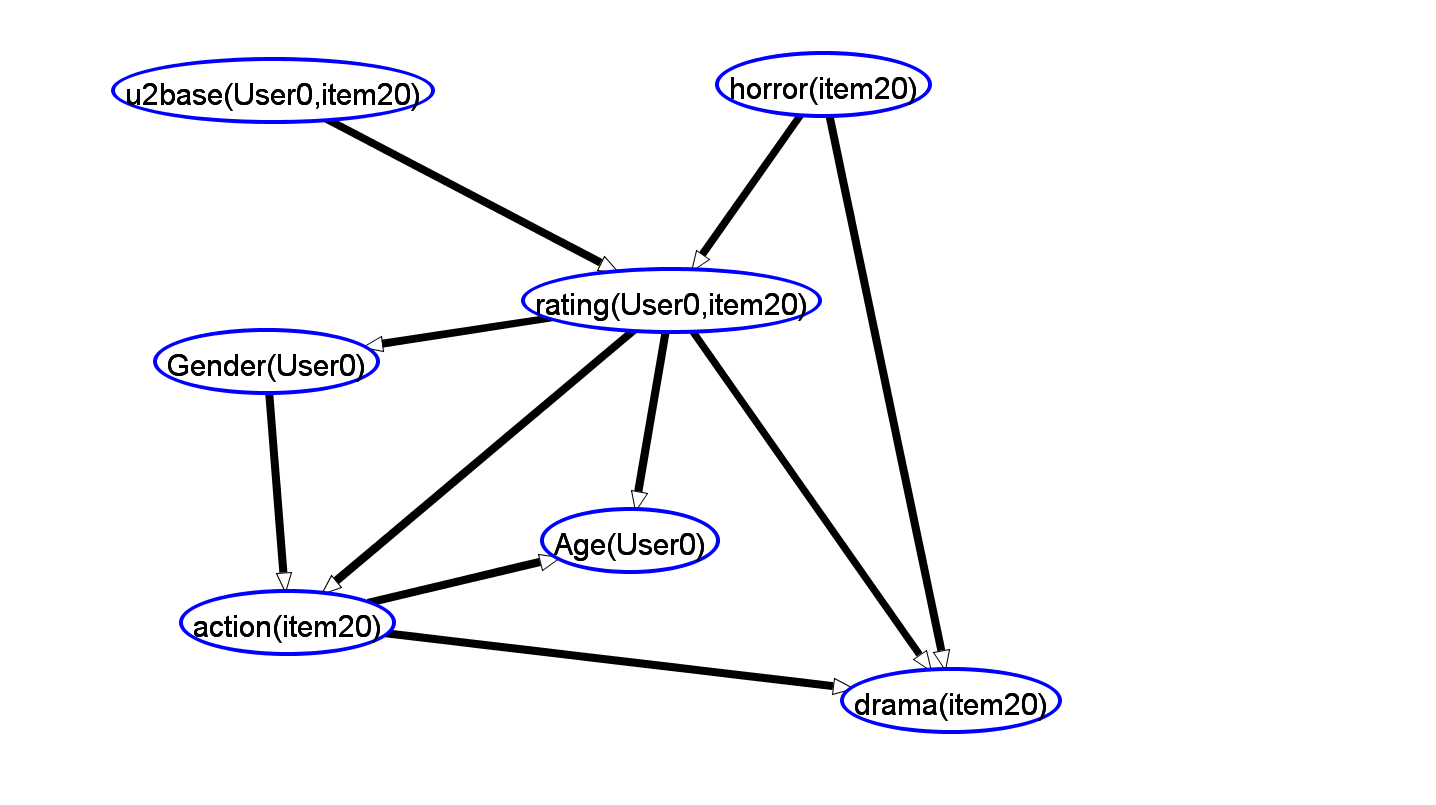
\includegraphics[width=7in,height=0.3\textheight]{movielens.png}
%%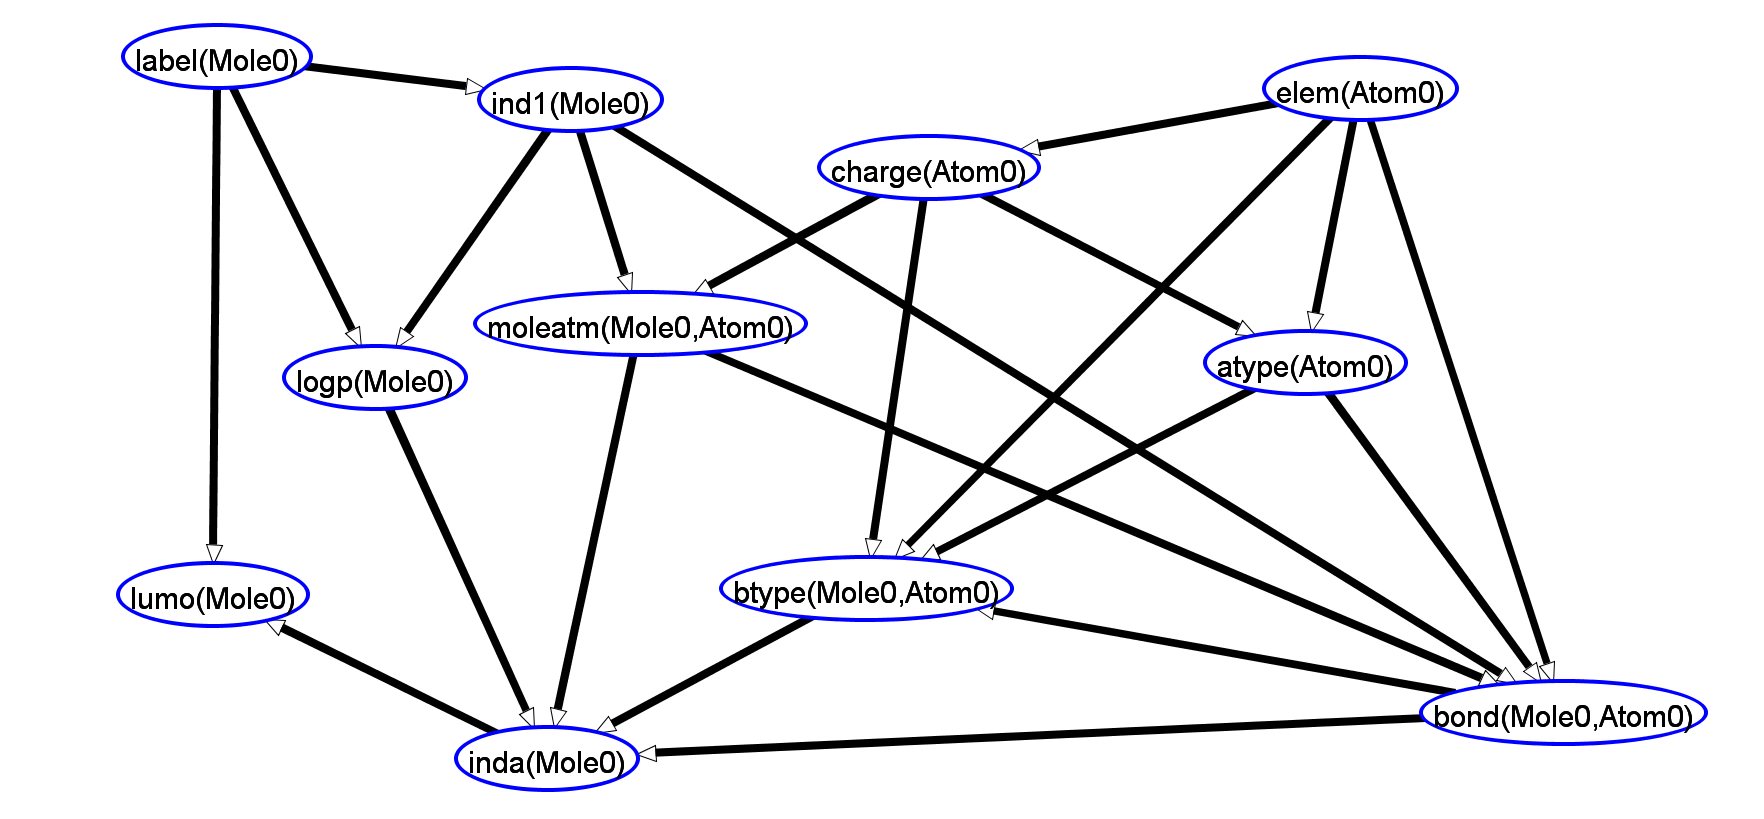
\includegraphics[width=7in,height=0.3\textheight]{muta.png}
%%
%%  \caption{Real Bayes Net Examples:.}
%%   \label{fig:BN_Examplse}
%%\end{figure*}
%
%
% The situation is reversed on the Mutagenesis dataset where flat search does well: compared to previous LAJ algorithm, %attribute-only search,
%it manages to fit the data better with a less complex model. 
%Hiearchical search performs very poorly compared to flat search (lower likelihood yet many more parameters in the model). Investigation of the models shows that the reason for this phenomenon is a special property of the Mutagenesis dataset: The two relationships in the dataset, Bond and MoleAtm, involve the same descriptive attributes. The hierarchical search learns two separate Bayes nets for each relationship, then propagates both sets to the final result. However, the union of the two graphs may not be a compact model of the associations that hold in the entire database. A solution to this problem would be to add a final pruning phase where redundant edges can be eliminated. We expect that with this change, hierarchical search would be competitive with flat search on the Mutagenesis dataset as well.
%
%
%


%%\section{Computing Relational Contingency Tables} \label{sec:cta}
%\section{Computing Contingency Tables For Positive Relationships} \label{sec:cta}
%
%
%%The learning algorithms described in this paper rely on the  availability of the $\ct$-tables (see Figure~\ref{fig:university-tables}). 
%%Computing the contingence tables raises two key challenges that we address in this paper. 
%If a conjunctive query involves only positive relationships, then it can be computed using SQL's sum aggregate function applied to a table join. The SQL sum query represents the positive part of the $\ct$-table much like a view definition represents a relation. 
%The challenge is generality: If the machine learning algorithm is developed without advance knowledge of the database schema, it needs to compute the SQL sum query from metainformation. 
%We propose accomplishing this via a \textbf{metaquery}.
%%: Using the meta-information in the random variable database, we construct an SQL query for each relationship chain. 
%%The SQL query represents a table join followed by a sum aggregation. Executing this query constructs the positive relationship part of the contingency table. 
%
%%In the next section we proposed a new approach for the second challenge.
%%
%%The second challenge is computing event counts that involve negated relationships. This is infeasible using standard table joins [explain: firends vs un-firends]. 
%%We approach this problem in two steps. 
%%First, we show that event counts using $m+1$ negated relationships can be computed from two event counts that each involve at most $m$ relationships. 
%%We state this result as a relational algebra identity in a new extension of relational algebra that we term \textbf{contingency table algebra}. A dynamic programming algorithm applies the algebraic identify repeatedly to efficiently build up a complete contingency table from partial tables that involve fewer negated relationships. 
%
%\subsection{Metaqueries for Utilizing Schema Information} 
%%As the top level of  Figure~\ref{fig:flow} illustrates, 
%The required counts involving only true relationships can be computed using the standard SQL constructs COUNT(*) and GROUP BY. 
%The general form of these operations is the same for every input database. 
%The varying part is the list of columns to be included, which depends on the input database. 
%For a fixed database, the column lists can be hard-coded. 
%To achieve a general solution when the column list is not known in advance, we introduce a new approach that we refer to as an SQL \textbf{meta query}. 
%
%An SQL meta query is an SQL query that takes as input schema information as recorded in the random variable database,
%and produces four kinds of tables: the Select, From, Where and Group By tables. The Select table lists the entries in the Select clause of the target query, the From table lists the entries in the From clause, and similar for Where and GROUP BY tables. %\footnote{basically the Group BY table is same as Select table without $\qcount$ column}. 
%%Thus an SQL meta query maps schema information to the components of another SQL query. 
%Given the four query tables, the corresponding SQL query can be easily executed in an application or stored procedure to produce the $\ct$-table entries.
%Figure~\ref{fig:meta-query} shows an example of meta queries for the university database.
%
%\begin{figure}[htb]
%\begin{center}
%\resizebox{0.5\textwidth}{!}{
%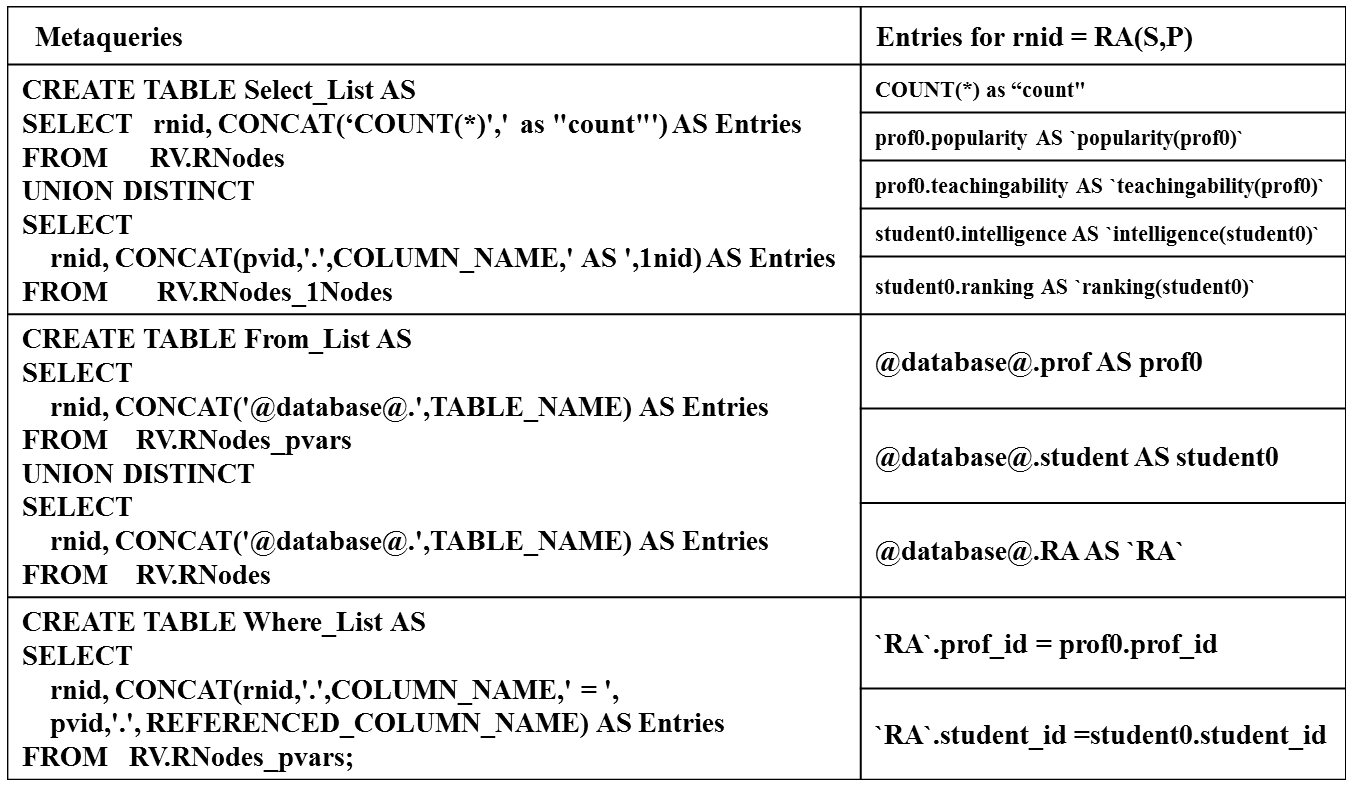
\includegraphics[width=0.5\textwidth]{figures/meta-query.png}
%}
%\caption{Example of Metaqueries and Entries for relationship table $\ra$ (i.e. rnid=$\ra$) based on university database.
%The entries of the Group By table (not shown) are the same as Select table but without $\qcount$ column.
%Here the $\it{@database@}$ is a variable denoting the given database schema.
%~\label{fig:meta-query} }
%\end{center}
%\end{figure}

%
%\section{Computing Contingency Tables For Negated Relationships} \label{sec:cta}
%
%Computing sufficient statistics that involve negated relationships is infeasible using standard table joins. 
%%and can be carried out by regular table joins or optimized virtual joins~\cite{Yin2004}. 
%%
%%Computing joint probabilities for a family containing one or more negative relationships is harder. 
%Standard join tables materialize new data tables that enumerate tuples of objects that are {\em not} related. %(see Figure~\ref{fig:university-tables}).
%%and then apply existing counting methods to the new tables. 
%However, the number of unrelated tuples is too large to make this scalable (think about the number of user pairs who are {\em not} friends on Facebook). 
%%A numerical example will illustrate why this is not feasible. Consider a university database with 20,000 Students, 1,000 Courses and 2,000 TAs. If each student is registered in 10 courses, the size of a $\it{Registered}$ table is 200,000. So the number of complementary student-course pairs is $2 \times 10^{7}-2 \times 10^{5}$, which is too big for most database systems. 
%%If we consider joins, complemented tables are even more difficult to deal with: suppose that each course has at most 3 TAs. Then  the number of satisfying instantiations of a positive relationship only formula such as $\it{Registered}(\S,\C) = \true,\it{TA}(\T,\C) = \true)$ is less than $6 \times 10^{5}$, whereas with negations the number of instantiations of the expression $\it{Registered}(\S,\it{course}) = \false, \it{TA}(\T,\it{course}) = \false)$ is on the order of $4 \times 10^{10}$. 
%%\subsection{The M\"obius parametrization.} 
%%To compute frequencies involving negated relationships, we would like to use the optimized algorithms for table join frequencies as an oracle/black box. 
%%Can we instead reduce the computation of sufficient statistics that involve negated relationships to the computation of sufficient statistics that involve existing (positive) relationships only? 
%%In their work on learning Probabilistic Relational Models with existence  uncertainty, Getoor et al. 
%%provided a subtraction method for the special case of estimating counts with only a single negated relationship \cite[Sec.5.8.4.2]{Getoor2007c}. 
%%They did not treat contingency tables with multiple negated relationships, which we consider next.
%
%We describe a ``virtual join'' algorithm that computes the required data tables without the quadratic cost of materializing a cross-product. Our experiments below compare the virtual joins with materializing table joins. 
%%We approach this problem in two steps. 
%First, we show that query counts using $m+1$ negated relationships can be computed from two query counts that each involve at most $m$ relationships. 
%We state this result as a relational algebra identity in a new extension of relational algebra that we term \textbf{contingency table algebra}. Second, a dynamic programming algorithm applies the algebraic identify repeatedly to efficiently build up a complete contingency table from partial tables.
%% that involve fewer negated relationships. 
%
%%Our first naive implementation constructs this tables using standard joins. 
%%While this was sufficient for our experiments, the cross-products carry a \textbf{quadratic} costs for binary relations, and therefore do not scale to large datasets. 
%%Moreover, the hierarchical search requires joins of the extended tables. 
%
%
%\textbf{to do: check page 19 of plan.pptx}
%%
%%Our starting point is the observation that a statistical learning algorithm like a Bayes net learner does not require an enumeration of individuals tuples, but only {\em sufficient statistics} \cite{Heckerman1995,Schulte2011}. 
%%These can be represented in {\em contingency tables} as follows \cite{Moore1998}. 
%%Consider a fixed list of relationship nodes $\R_{1}, R_{2},\ldots,R_{m}$, and attribute nodes $\functor_{1},\ldots,\functor_{j}$. 
%%A \textbf{query} is a set of $(node = value)$ pairs where each value is of a valid type for the node. 
%%The \textbf{result set} of a query in a database $\D$ is the set of instantiations of the population variables such that the query evaluates as true in $\D$.
%%For example, in the database of Figure~\ref{fig:university-tables} the result set for the query 
%%$(\it{intelligence}(\S) = 2$, $\it{rank}(\S) = 1$, $\it{rating}(\C) = 3$, $\it{Diff}(C) = 1$, $\reg(\S,\C) = F)$ 
%%is the singleton $\{\langle \it{kim}, \it{101}\rangle\}$. 
%%The \textbf{count} of a query is the cardinality of its result set. 
%%Each subset of nodes $\set{V} = v_{1},\ldots,v_{n}$ has an associated \textbf{contingency table} denotes by $\cttable(\set{V})$. %$CT(\set{V})$. 
%%This is a table with a row for each of the possible assignments of values to the nodes in $\set{V}$, and a special integer column called $\qcount$. 
%%The value of the $\qcount$ column in a row corresponding to $V_{1} = v_{1},\ldots,V_{n} = v_{n}$ records the count of the corresponding query. 
%%Figure~\ref{fig:ct} shows a partial contingency table from University database.
%
%
%
%
%
%\subsection{Contingency Table Algebra} 
%%\subsection{Definition} 
%First we introduce some notation.
%If $\dtable$ denotes a generic database table, then $\ColumnList(\dtable)$ is a list of columns in table $\dtable$; the list order is irrelevant. For a CT-table $\ct$, the expression $\ColumnList(\ct)$ denotes a list of columns other than the count column.
%
%none $\qcount$ columns in table $\dtable$, 
%and column sets $\set{V}$, $\set{U}$ are the union of $ \qcount $ column with $\ColumnList({\dtable})$ for different given $\dtable$. 
%Suppose ${\dtable}_{1}$, ${\dtable}_{2}$ be two union-compatible %contingency 
%tables with the same column headers, and ${\dtable}_{3}$ is another table,
%then $\ColumnList({\dtable}_{1}) =V_{1}, \ldots,\ V_{k}$, $\ColumnList({\dtable}_{2}) =V_{1}, \ldots,\ V_{k}$
%and $\ColumnList({\dtable}_{3}) = U_{1}, \ldots,\ U_{m}$.
%We define $\ColumnList({\dtable}_{1}) = \ColumnList({\dtable}_{2})$ by 
%${\dtable}_{1}.V_{1} ={\dtable}_{2}.V_{1}, \ldots, {\dtable}_{1}.V_{k} = {\dtable}_{2}.V_{k}$.
%
%
%\textbf{to do: %update the $CL$, $\cup$,
% check the consistency with algorithm part?}
%
%\subsubsection{Unary Operators} \label{sec:unary}
%\begin{description}
%\item[Selection] $\sigma_{\selectcond}  \ct$ selects a subset of the rows in the  $\ct$-table  that satisfy condition $\selectcond$. This is the standard relational algebra operation except that the selection condition $\selectcond$ may not involve the $\qcount$ column.
%\item[Projection]  %$\project_{\set{V}}  
%$\project_{\V_{1},\ldots,\V_{k}} \ct$ selects a subset of the  columns in the  $\ct$-table, excluding the count column. 
%The counts in the projected subtable are the sum of counts of rows that satisfy the query in the subtable. 
%The  $\ct$-table projection  $\project_{\V_{1},\ldots,\V_{k}} \ct$ can be defined by the following pseudo-SQL code:
%
%\begin{quote}
%SELECT SUM(COUNT) AS COUNT, $V_{1}, \ldots,\ V_{k}$ \\
%FROM $\cttable$ \\
%GROUP BY $V_{1}, \ldots,\ V_{k}$
%\end{quote}
%%\begin{quote}
%%SELECT SUM($\qcount$) AS $\qcount$, $\ColumnList({\ct})$ \\
%%FROM $\ct$ \\
%%GROUP BY $\ColumnList({\ct})$
%%\end{quote}
%
%
%\item[Conditioning]  $\condition_{\selectcond}  \ct$ returns a conditional contingency table. Ordering the columns as $(V_{1},\ldots,V_{i}, \ldots,\V_{i+j}$),  suppose that the selection condition is a conjunction of values of the form $C = (V_{i+1} = v_{i+1},\ldots, V_{i+j} = v_{i+j})$.  Conditioning can be defined in terms of selection and projection by the equation:
%\begin{equation}
%\condition_{\selectcond}  \ct = \project_{\V_{1},\ldots,\V_{i}} (\select_{\selectcond}  \ct) \nonumber
%\end{equation}
%\end{description}
%
%\subsubsection{Binary Operators} \label{sec:bin}
%
%\begin{description}
%\item[Cross Product]  %Let %$\ct_{1}(\V_{1}, \ldots,\ V_{m}),\ct_{3}(U_{1}, \ldots,\ U_{k})$
%%$\ct_{1}(\set{V}),\ct_{3}(\set{U})$ 
%% be two contingency tables %that do not share any papulation variable. 
%The \textbf{cross-product} of $\ct_{1}(\set{U}),\ct_{2}(\set{V})$ is the Cartesian product of the rows, where the product counts are the products of count. The cross-product can be defined by the following pseudo-SQL code:
%% \begin{quote}
%%SELECT \\($\ct_{1}.COUNT*\ct_{2}.COUNT$) AS COUNT,  $U_{1}, \ldots,\ U_{k}, \V_{1}, \ldots,\ V_{m}$ \\
%%FROM  $\ct_{1},\ct_{2}$
%%\end{quote}
%\begin{quote}
%SELECT \\($\ct_{1}.\qcount *\ct_{2}.\qcount$) AS $\qcount$,  $\ColumnList({\ct_{1}}), \ColumnList({\ct_{2}}) $\\
%FROM  $\ct_{1},\ct_{2}$
%\end{quote}
%
%
%\item[Addition] 
% The \textbf{count addition} $\ct_{1}(\set{V}) + \ct_{2}(\set{V})$ adds the counts of matching rows, as in the following pseudo-SQL query.
%\begin{quote}
%SELECT % $\ct_{1}$.COUNT+$\ct_{2}$.COUNT 
%$\ct_{1}.\qcount$+$\ct_{2}.\qcount$ AS $\qcount$, $\ColumnList({\ct_{1}})$ \\%$\ct_{1}.V_{1} , \ldots, \ct_{1}.V_{k} $ \\
%FROM  $\ct_{1},\ct_{2}$\\
%%WHERE $\ct_{1}.V_{1} = \ct_{2}.V_{1}, \ldots, \ct_{1}.V_{k} = \ct_{2}.V_{k}$
%WHERE $\ColumnList({\ct_{1}}) = \ColumnList({\ct_{2}})$
%\end{quote}
%
%If a row appears in one $\ct$-table but not the other, we include the row with the count of the table that contains the row. Note that  $\ct_{1}(\set{V})$ and $\ct_{2}(\set{V})$ are union-compatible because they have the same  column headers.
%
%\item[Subtraction] %Let $\ct_{1}(\set{V}),\ct_{2}(\set{V})$ be two union-compatible contingency tables with the same column headers. 
%The \textbf{count difference} $\ct_{1}(\set{V}) - \ct_{2}(\set{V})$ equals $\ct_{1}(\set{V}) + (- \ct_{2}(\set{V}))$ where $- \ct_{2}(\set{V})$ is the same as $\ct_{2}(\set{V})$ where the counts are negative. 
%Table subtraction is defined only if (i) without the $\qcount$ column, the rows in $\ct_{1}$ are a superset of those in $\ct_{2}$, and (ii) for each row that appears in both tables, the count in $\ct_{1}$ is at least as great as the count in $\ct_{2}$.
%
%
%\end{description}
%
%
%%\subsection{Implementing the Contingency Table Operators}\label{sec:imp}
%%Everything true: database optimization. General tricks, e.g., omit 0 counts. Specific tricks, e.g. merge-sort.
%\subsubsection{Implementation}\label{sec:imp}
%Our implementation is based on SQL queries, whose execution is well optimized by a RDBMS such as MySQL.   
%A RDBMS offers built-in options for improving query planning, such as using covering index  to speed up the conditioning.
%%[give examples: e.g, indixes]. 
%For some operations where MySQL chooses a suboptimal query plan, we implemented our own method.
%
%%\subsubsection{Unary Operators}
%%Suppose we already know the required columns list $\ColumnList({\dtable})$ for each query clause. 
%The selection operator can be implemented  using SQL as with standard relational algebra. 
%Project with $\ct$-tables requires use of the GROUP BY construct as shown in Section~\ref{sec:unary}. 
%%The list of columns to be projected at a point in the algorithm can be found by a meta query. 
%%\subsubsection{Binary Operators}
% % big * smaller, faster enough.
%%The required column lists can be found by a meta query. 
%
%The most difficult operation to implement efficiently is 
%For addition/subtraction, simply executing the SQL query shown above %shown in Section~\ref{sec:bin} 
%may lead to a \textbf{quadratic} cost if a nested-loops join is used, and therefore does not scale to large datasets.
%The most efficient algorithm is a sort-merge join \cite{Ullman1982}. 
%Given two union-compatible $\ct$-tables, each row in one matches at most one other on the non-count columns. 
%As is well known, with unique matches, the cost of a sort-merge join is $\it{size}(table1) + \it{size}(table2) +$ the cost of sorting both tables. 
%Our experiments below are based on a sort-merge join (our own implementation in Java). The cross product is easily implemented in SQL as shown in Section~\ref{sec:bin}. However, the cross product size is quadratic in the size of the input tables, so a quadratic cost is unavoidable.
%%A general trick to shrink the size $\ct$-table is remove the 0 counts in $\ct$-table.
%%But for a general input database, usually the user can not know the column lists in advance. 
%%So in next section, we propose a new method to compute these.
%
%
%

%
%\subsection{Latttice Computation of Contingency Tables} \label{sec:mobius}
%%\textbf{older material}
%%Our flat search algorithm can be implemented by computing the contingency table for all functor nodes, then presenting it to a Bayes net learner. 
%%The hierarchical search algorithms can be implemented by computing the contingency tables for each relationship chain in the lattice (Figure~\ref{fig:big-lattice}). 
%%For a relationship set, the nodes in the contingency table comprise (1) the descriptive attributes of the entities involved in the relationship set, 
%%(2) the descriptive attributes of the relationships, and (3) a Boolean relationship node for each member of the set. 
%This section describes a method for computing the contingency tables level-wise in the relationship chain lattice. We start with a contingency table algebra equivalence that allows us to compute counts for rows with negative relationships from rows with positive relations.
%
%%
%%\textbf{old material} So long as a database probability involves only positive relationships,
%%%formula only contains positive relationships, 
%%%the computation is straightforward. 
%%%For example, in 
%%%$P_{\D}(\it{gender}(\X) = M, \it{Friend}(\X,\Y) = \true)$, the value  $\grounds_{\D}(\it{gender}(\X) = M, \it{Friend}(\X,\Y) = \true)$, the count of friendship pairs $(x,y)$ where $x$ is male and the
%%%{\em Friend} relationship is true, 
%%and can be carried out by regular table joins or optimized virtual joins~\cite{Yin2004}. 
%%%
%%Computing joint probabilities for a family containing one or more negative relationships is harder. 
%%A naive approach would explicitly construct new data tables that enumerate tuples of objects that are {\em not} related. %(see Figure~\ref{fig:university-tables}).
%%%and then apply existing counting methods to the new tables. 
%%However, the number of unrelated tuples is too large to make this scalable (think about the number of user pairs who are {\em not} friends on Facebook). 
%%A numerical example will illustrate why this is not feasible. Consider a university database with 20,000 Students, 1,000 Courses and 2,000 TAs. If each student is registered in 10 courses, the size of a $\it{Registered}$ table is 200,000. So the number of complementary student-course pairs is $2 \times 10^{7}-2 \times 10^{5}$, which is too big for most database systems. 
%%If we consider joins, complemented tables are even more difficult to deal with: suppose that each course has at most 3 TAs. Then  the number of satisfying instantiations of a positive relationship only formula such as $\it{Registered}(\S,\C) = \true,\it{TA}(\T,\C) = \true)$ is less than $6 \times 10^{5}$, whereas with negations the number of instantiations of the expression $\it{Registered}(\S,\it{course}) = \false, \it{TA}(\T,\it{course}) = \false)$ is on the order of $4 \times 10^{10}$. 
%%\subsection{The M\"obius parametrization.} 
%%To compute frequencies involving negated relationships, we would like to use the optimized algorithms for table join frequencies as an oracle/black box. 
%%Can we instead reduce the computation of sufficient statistics that involve negated relationships to the computation of sufficient statistics that involve existing (positive) relationships only? 
%%In their work on learning Probabilistic Relational Models with existence  uncertainty, Getoor et al. 
%%provided a subtraction method for the special case of estimating counts with only a single negated relationship \cite[Sec.5.8.4.2]{Getoor2007c}. 
%%They did not treat contingency tables with multiple negated relationships, which we consider next.
%
%\textbf{need to define *. Point to example in diagram}
%
%\begin{proposition}%[Pivot_CT]
%\label{PivotCT}
%Let $R$ be a relationship node and let $\set{R}$ be a set of relationship nodes. Let $\Nodes$ be a set of nodes that %(1) must contain all $\eatts$ of $\R$, and may contain any other nodes, as long as (2) $\Nodes$ 
%does not contain $\R$ nor any of the $\ratts$ of $\R$. Let  $\X_{1},\ldots, \X_{l}$ be the population variables that appear in $\R$ but not in $\Nodes$ where ${l}$ is a number could be zero. Then we have
%\begin{flalign}
%\label{update}
%&\ct(\Nodes \cup \eatts(R)|\set{R} = \true, R = F) = & \\ %\nonumber\\
%& \ct(\Nodes|\set{R} = \true, R =*) \times \ct(\X_{1}) \times \cdots \times \ct(\X_{l}) \nonumber & \\
%& -\ct(\Nodes  \cup \eatts(R)|\set{R} = \true, R = T). \nonumber&
%\end{flalign}
%If $l = 0$, the equation holds without  the %$ \ct(\X_{1}) \times \cdots \times \ct(\X_{k})$ 
%cross-product term.
%
%\end{proposition}
%
%
%\begin{proof}
%The equation 
%\begin{align}
%&\ct(\Nodes  \cup \eatts(R)|\set{R} = \true, R = *) = &\label{eq:update}  \\ 
%&\ct(\Nodes  \cup \eatts(R)|\set{R} = \true, R = T)  + & \nonumber \\ 
%&\ct(\Nodes  \cup \eatts(R)|\set{R} = \true, R = F) & \nonumber
%\end{align}
%holds because the set $\Nodes \cup \eatts(R)$ contains all population variables in $R$ by the assumption that each population variable is associated with at least one $\eatt .$ % $\it{1Node}$. 
%
%%Using table subtraction Equation~\eqref{eq:update} implies
% Equation~\eqref{eq:update} implies
%\begin{align} 
%&\ct(\Nodes  \cup \eatts(R)|\set{R} = \true, R = \false) =& \label{eq:table-subtract} \\ 
%&\ct(\Nodes  \cup \eatts(R)|\set{R} = \true, R = *) -&\nonumber  \\
% & \ct(\Nodes  \cup \eatts(R)|\set{R} = \true, R = \true).& \nonumber
%\end{align}
%
%To compute the CT-table conditional on the relationship $\R$ being unspecified, we use the equation
%\begin{align}
%&\ct(\Nodes  \cup \eatts(R)|\set{R} = \true, R = *) =  &\label{eq:table-multiply}\\
%&\ct(\Nodes|\set{R} = \true, R =*) \times \ct(\X_{1}) \times \cdots \times \ct(\X_{l})& \nonumber
%\end{align}
%which holds because if the set $\Nodes$ does not contain a population variable of $\R$, then the counts of the associated $\eatts(\R)$ are independent of the counts for $\Nodes$. 
%If $l = 0$, this means there's no new papulation variable introduced, Equations~\eqref{eq:table-multiply} holds without  the cross-product term.
%
%Together Equations~\eqref{eq:table-subtract} and~\eqref{eq:table-multiply} establish the proposition \ref{PivotCT}.
%\end{proof}
%
%Algorithm ~\ref{Pivot_CT_Computation} provides pseudo-code for applying Equation~\eqref{eq:update} to compute a complete CT-table given a partial table where a specified relationship node $\Relation$  is true and another partial table that does not contain the relationship node. We refer to $\Relation$ as the \textbf{pivot} node. For extra generality, we apply the Equation with a condition that lists a set of relationship nodes fixed to be true. 
%
%Algorithm~\ref{level-wise-subtract} shows how the Pivot operation can be applied repeatedly to find all contigency tables in the relationship lattice. 
%
%\begin{enumerate}
%\item Compute $\ct$-tables for entities (lines 1--3).
%\item Compute $\ct$-tables for each single relationship node (lines 4--8).
%\begin{enumerate}
%\item Where the relationship value is unspecified, the $\ct$-table is the cross-product of the $ct$-tables for the entity tables involved in the relationship (line 5).
%\item Where the relationship value is specified as true, the $\ct$-table can be found  using an SQL metaquery (line 6).
%\item Apply the Pivot function to construct the  complete $\ct$-table from the previous two tables (line 7).
%\end{enumerate}
%\item Compute $\ct$-tables for all relationship chains of length $>1$ (lines 9--23).
%\begin{enumerate}
%\item For each relationship chain, find the conditional $\ct$-table where all relationship nodes are specified as true (line 11). 
%\item Order the relationship nodes in the chain arbitrarily. Make each relationship node in order the Pivot node $\Relation_{i}$.
%\item For the current Pivot node $\Relation_{1}$, find the conditional $\ct$-table where $\Relation_{i}$ is unspecified, and the following relations $\Relation_{j}$ with $j>i$ are true (lines 14--19). (This can be computed from a $ct$-table for a shorter chain that has been constructed already.)
%\item The $ct$-table condition on $\Relation_{i}$ and the following relations being true has been constructed already (see loop invariant). Apply the Pivot function to construct the  complete $\ct$-table, conditional on the following relations being true (line 20).
%\end{enumerate}
%\end{enumerate}
%
%
%
%
%
%Algorithm ~\ref{Pivot_CT_Computation} and~\ref{level-wise-subtract} present the fast computation for given length of relationship chain.
%
%The Virtual Join algorithm requires support for two basic tasks: 1) compute initial $\ct$-tables from the base data tables, 
%and 2) apply CT-algebra operations to form new CT-tables from existing ones. %We discuss these in turn.
%
%Figure~\ref{fig:flow} illustrates the computation using  contingency table algebra when there's only one relationship.


%
%
%\begin{figure*}[tb]
%\begin{center}
%\resizebox{0.9\textwidth}{!}{
%%%!%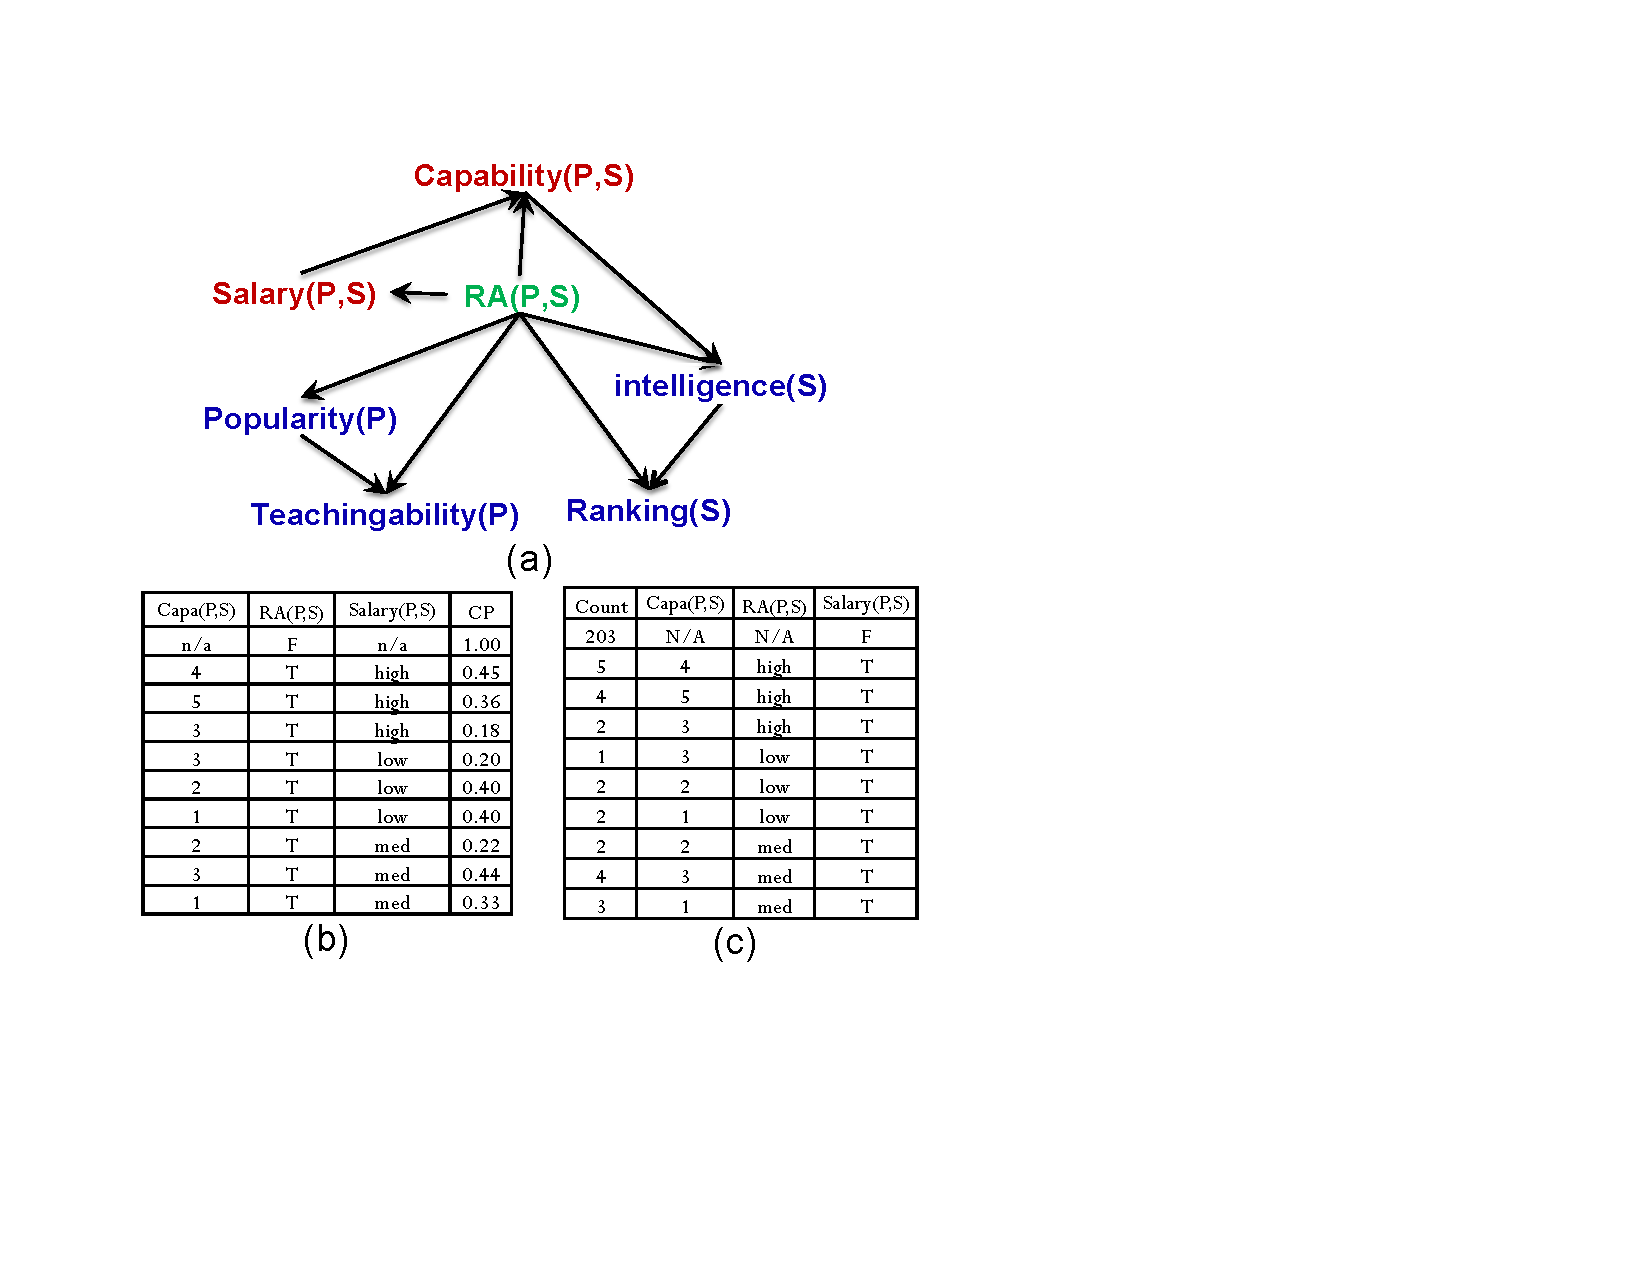
\includegraphics[width=1\textwidth]{pbn}
%%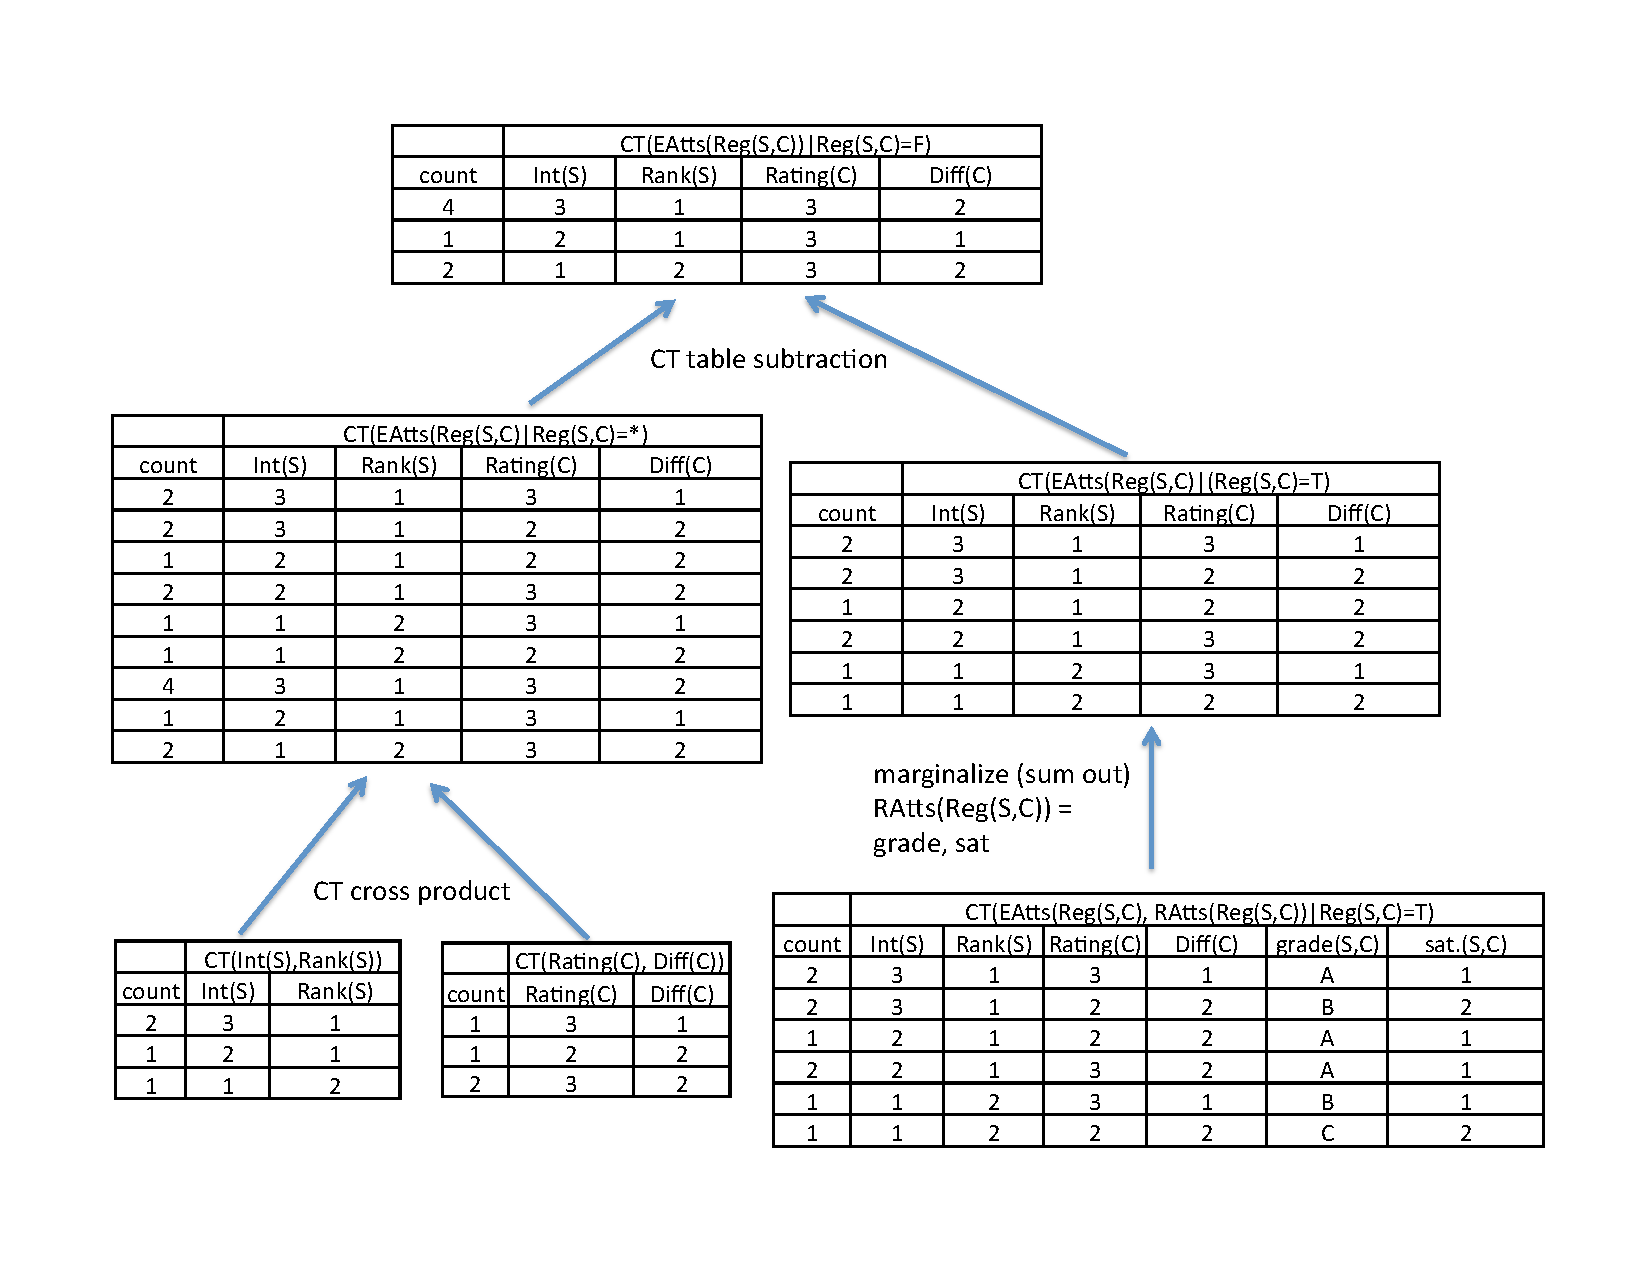
\includegraphics{figures/subtraction-flow.pdf}
%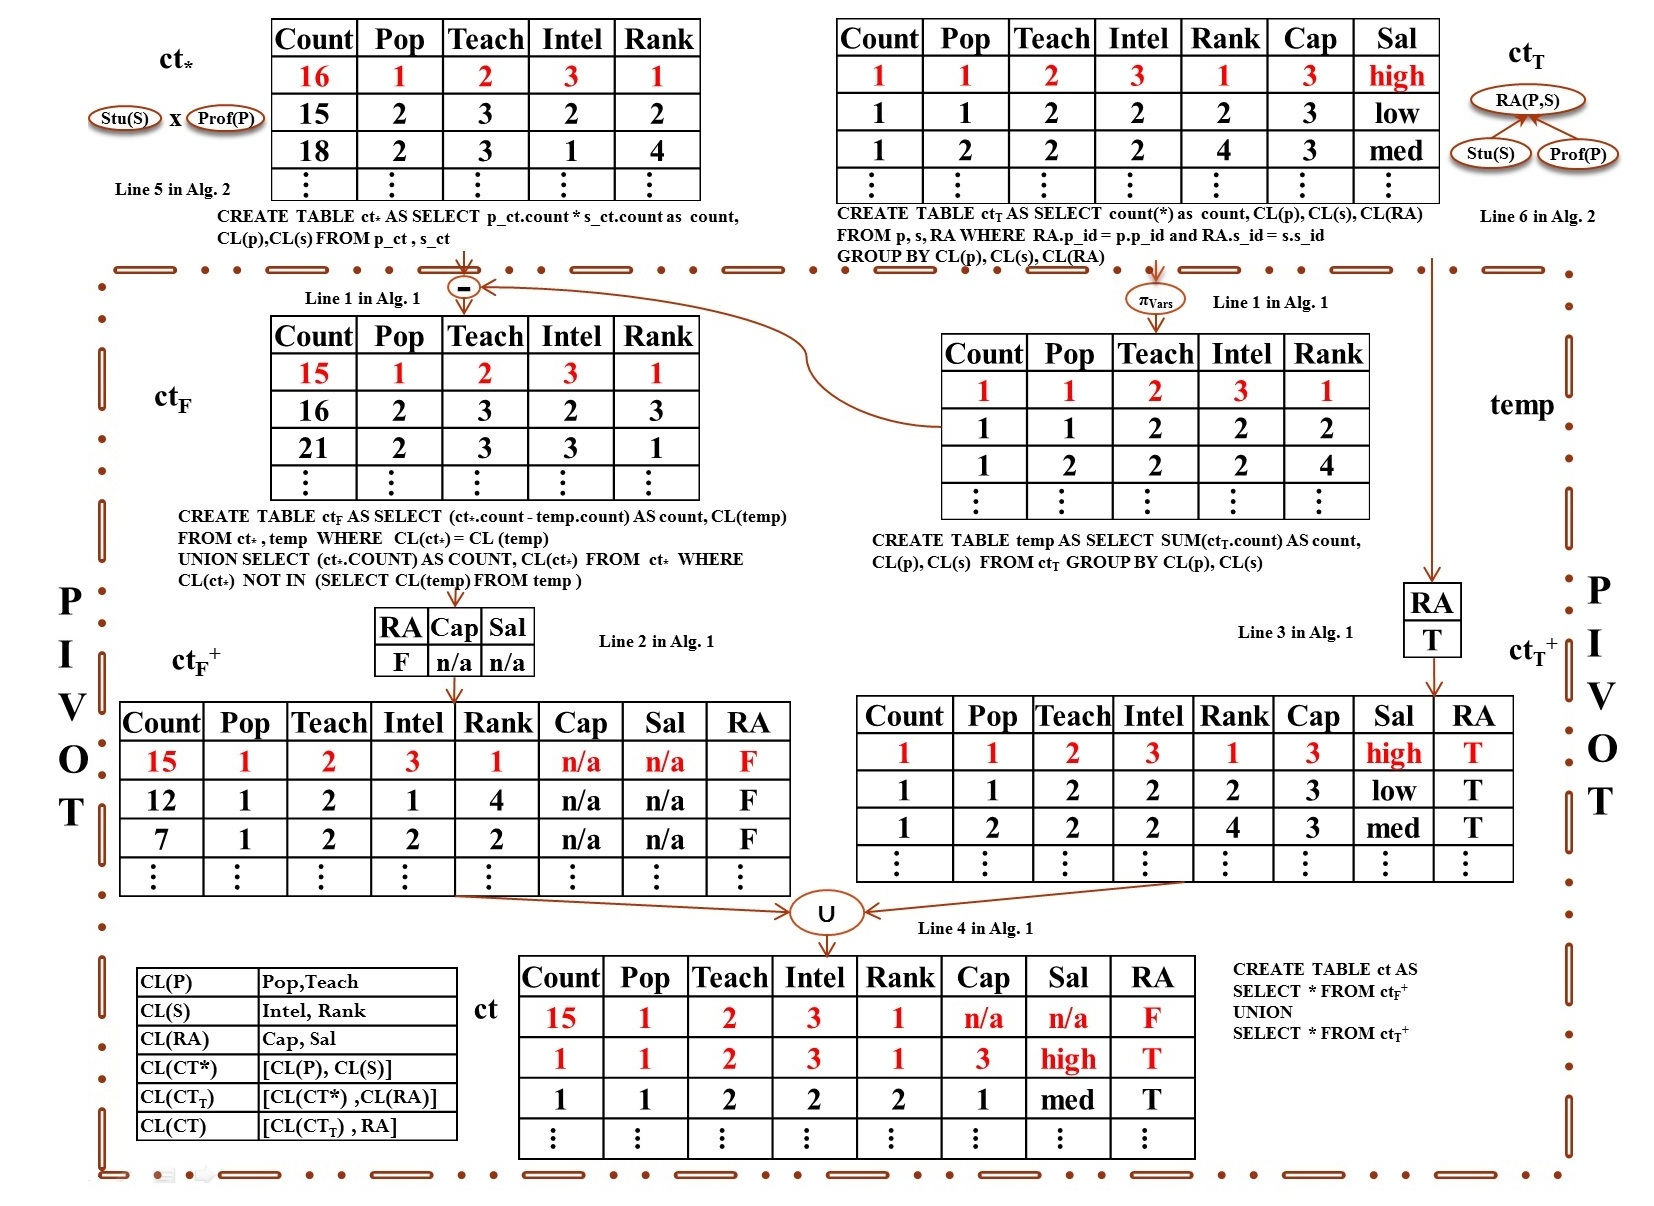
\includegraphics[width=0.9\textwidth]{figures/sub.jpg}
%}
%\caption{Examples of the contingency table algebra operations  following Proposition~\ref{PivotCT} %and equations
%based on partial University database with SQL queries. %[Column-List(TABLE)].
%$\ColumnList({p})= Pop, Teach; \ColumnList({s}) = Intel, Rank;\ColumnList({RA})= Cap, Sal; \ColumnList({CT_{*}}) = \ColumnList({temp}) = Pop, Teach, Intel, Rank; \ColumnList({CT_{T}}) = Pop, Teach, Intel, Rank, Cap, Sal;\ColumnList({CT_{F}}) = Pop, Teach, Intel, Rank;$
%$\ColumnList({CT}) =  \ColumnList(CT_{\false}^{+})  = \ColumnList(CT_{\true}^{+}) = Pop, Teach, Intel, Rank, Cap, Sal, RA.$ to do: change the place?
%\label{fig:flow}}
%\end{center}
%\end{figure*}
%
%
%\begin{algorithm*}[htbp]
%\label{Pivot_CT_Computation}
%%\linesnumbered
%\SetKwData{KwCalls}{Calls}
%\SetKwData{KwCondition}{Precondition:}
%\KwIn{Two conditional contingency tables   $CT_{\true} :=\ct(\it{Nodes},\it{\ratts}(R_{\it{pivot}})|R_{\it{pivot}}=\true$$,\vec{R}=\true)$ and  $CT_{*} :=\ct(\it{Nodes}|R_{\it{pivot}} = *$$,\vec{R}=\true)$ .}
%\KwCondition  %$\it{Nodes}:= \eatts(\R_{1},\ldots,\R_{\ell}) \cup \ratts(\R_{1},\ldots,\R_{\ell}) \cup (\R_1,\ldots,\R_{\ell}) - R_{\it{pivot}} - \ratts(R_{\it{pivot}}) $ \;
% The set $\it{Nodes}$ does not contain the relationship node $R_{\it{pivot}}$ nor any of its descriptive attributes $\ratts(R_{\it{pivot}}$).
%
%% {The set $\it{Nodes}$ contains $\eatts(\R_{1},\ldots,\R_{\ell}) \cup \ratts(\R_{1},\ldots,\R_{\ell}) \cup (\R_1,\ldots,\R_{\ell})$ but not the relationship node $R_{\it{pivot}}$ nor any of its descriptive attributes $\ratts(R_{\it{pivot}}$) \;}
%
%\KwOut{The conditional contigency table $ \ct(\it{Nodes},\it{\ratts}(R_{\it{pivot}}),R_{\it{pivot}}|$$\vec{R}=\true)$ .}
%\begin{algorithmic}[1]
%%\STATE $CT_{\false} := \ct(\it{Nodes}|R_{\it{pivot}} = *$$,\vec{R}=\true) - \pi_{\it{Nodes}} \ct(\it{Nodes},\it{\ratts}(R_{\it{pivot}})|R_{\it{pivot}}=\true$$,\vec{R}=\true)$.
%\STATE $CT_{\false} := CT_{*} - \pi_{\it{Nodes}}CT_{\true}$.
%
%\COMMENT{ Implements the algebra Equation~\ref{update}  in proposition~\ref{PivotCT}. }
%\STATE $CT_{\false}^{+}$ := extend  $CT_{\false}$ with columns $R_{\it{pivot}}$ everywhere false and $\it{\ratts}(R_{\it{pivot}})$ everywhere $n/a$.
%%\STATE $CT_{\true}^{+}$ := extend  $\ct(\it{Nodes},\it{\ratts}(R_{\it{pivot}})|R_{\it{pivot}}=\true$$,\vec{R}=\true)$ with columns $R_{\it{pivot}}$ everywhere true.
%\STATE $CT_{\true}^{+}$ := extend  $CT_{\true}$ with columns $R_{\it{pivot}}$ everywhere true.
%\STATE \Return $CT_{\false}^{+} \cup CT_{\true}^{+}$
%\end{algorithmic}
%\label{alg:pivot}
%\caption{The Pivot function returns a conditional contingency table for a set of attribute nodes and all possible values of the relationship $R_{\it{pivot}}$, including $R_{\it{pivot}} = \false$. %It implements the algebra Equation~\eqref{eq:update}.
% The set of conditional relationships $\vec{R} =(\R_{pivot},\ldots,\R_{\ell})$ %=\true$
% may be empty in  which case the Pivot computes an unconditional CT-table. }
%\end{algorithm*}
%
%
%
%
%\begin{algorithm*}[htbp]
%\label{level-wise-subtract}
%%\linesnumbered
%\SetKwData{KwCalls}{Calls}
%\SetKwData{Notation}{Notation}
%\KwIn{A relational database $\D$; a set of functor nodes}
%\KwOut{A contingency table that lists the count in the database $D$ for each possible assignment of values to each functor node.}
%%\KwCalls  Pivot
%\begin{algorithmic}[1]
%\FORALL{population variables $\X$}
%\STATE compute $\ct(\eatts(\X))$ using SQL queries.
%\ENDFOR
%
%\FORALL{relation node $\R$}
%\STATE $CT_{*} := \ct(\X) \times \ct(\Y)$ where $\X$,$\Y$ are the population variables in $\R$.
%\STATE $CT_{\true} := \ct(\eatts(\R)|\R = \true)$ using SQL joins.
%\STATE Call  $\it{Pivot}(CT_{\true},CT_{*})$ to compute $\ct(\eatts(\R),\ratts(\R),\R)$.
%% with the two tables $CT_{*}$ and $CT_{\true}$  
%\ENDFOR
%
%\FOR{Rchain length $\ell=2$ to $m$}
%\FORALL{Rchain $\R_{1},\ldots,\R_{\ell}$}
%
%\STATE $Current\_CT :=  \ct(\eatts(\R_{1},\ldots,\R_{\ell}), \ratts(\R_{1},\ldots,\R_{\ell})|\R_{1}=\true,\ldots,\R_{\ell}=\true)$ using SQL joins.
%%\STATE $CT_{*} := \ct(\eatts(\R_{2},\ldots,\R_{\ell}), \ratts(\R_{2},\ldots,\R_{\ell})|
%%\R_{1}=*,\R_{2} = \true,\ldots,\R_{\ell}=\true) \times \ct(\X)$ where $\X$ is the population variable in $\R_{1}$, if any, that does not appear in $\R_{2},\ldots,\R_{\ell}$\; 
%%\COMMENT{$CT_{*}$ can be computed from a CT-table for a Rchain of length $\ell-1$.}
%%\STATE  $Current\_CT :=  \it{Pivot}(Current\_CT,CT_{*})$ \;
%%\COMMENT{The table $Current\_CT$ equals $ \ct(\eatts(\R_{1},\ldots,\R_{\ell}), \ratts(\R_{1},\ldots,\R_{\ell})
%%,\R_{1}|\R_{2} = \true,\ldots,\R_{\ell}=\true)$.}
%\FOR{$i=1$ to $\ell$} \label {refline:innerloop}
%\IF{ $i$ equals  1}
%\STATE $CT_{*} := \ct(\eatts(\R_{2},\ldots,\R_{\ell}), \ratts(\R_{2},\ldots,\R_{\ell})|
%\R_{1}=*,\R_{2} = \true,\ldots,\R_{\ell}=\true) \times \ct(\X)$ where $\X$ is the population variable in $\R_{1}$, if any, that does not appear in $\R_{2},\ldots,\R_{\ell}$\; 
%\COMMENT{$CT_{*}$ can be computed from a CT-table for a Rchain of length $\ell-1$.}
%\ELSE
%\STATE $\eatts_{\bar{i}} := \eatts(\R_{1},\ldots,\R_{i-1},\R_{i+1},\ldots,\R_{\ell})$.
%\STATE $\ratts_{\bar{i}} := \ratts(\R_{1},\ldots,\R_{i-1},\R_{i+1},\ldots,\R_{\ell})$.
%%\STATE $\ratts_{i} := \ratts(\R_{1},\ldots,\R_{i-1},\R_{i+1},\ldots,\R_{\ell})$.\
%%\STATE $\it{Nodes_{i}} := \eatts \cup \ratts_{i} \cup \{\R_{1},\ldots,\R_{i-1}\}$.
%%\STATE $\vec{\R} := \{\R_{i+1},\ldots,\R_{\ell}\}$.
%\STATE $CT_{*} := \ct(\eatts_{\bar{i}}, \ratts_{\bar{i}},\R_{1},\ldots,\R_{i-1})|
%\R_{i}=*,\R_{i+1} = \true,\ldots,\R_{\ell}=\true) \times \ct(\Y)$ where $\Y$ is the population variable in $\R_{i}$, if any, that does not appear in $\vec{\R}$. 
%\ENDIF \\
%%\COMMENT{$\vec{R}$ is an Rchain of length $\ell-i$, so the CT-table $ \ct(\eatts,\ratts($$\vec{\R}))$ has been computed already.}
%%\IF{ $i$ equals to 1}
%%\STATE   $CT_{\true} = \ct(\it{Nodes_{i}},\ratts(\R_{i})|\R_{i} = \true,$$\vec{\R} = \true)$ using SQL joins.
%%\ELSE
%%\STATE   $CT_{\true} :=CT_{i-1}$.
%%\COMMENT{updating the $CT_{\true}$ with the $CT_{i-1}$ just computed in previous loop.}
%%\ENDIF \\
%\STATE $Current\_CT :=  \it{Pivot}(Current\_CT,CT_{*})$.
%% with the two tables $CT_{*}$ and $CT_{\true}$  to compute $\ct(\it{Nodes_{i}},\ratts(\R_{i}),\R_{i}|$$\vec{\R} = \true)$.
%\ENDFOR
%
%\COMMENT{Loop Invariant: After  iteration $i$, the table $Current\_CT$ equals $ \ct(\eatts(\R_{1},\ldots,\R_{\ell}), \ratts(\R_{1},\ldots,\R_{\ell})
%,\R_{1},\ldots,\R_{i}|
%\R_{i+1} = \true,\ldots,\R_{\ell}=\true)$}
%%After $i = \ell$, we have computed  $\ct(\eatts(\R_1,\ldots,\R_{\ell}),\ratts(\R_1,\ldots,\R_{\ell}),\R_1,\ldots,\R_{\ell})$}
%
%\ENDFOR
%
%\COMMENT{Loop Invariant: The CT-tables for all Rchains of length $\ell$ have been computed.}
%
%\ENDFOR 
%
%\STATE \Return the CT-table for the Rchain involves all the relationship nodes.
%\end{algorithmic}
%\label{alg:fmt}
%\caption{Virtual Join Algorithm for Computing the Contingency Table for Input Database}%Dynamic Algorithm for Computing  {\em Sufficient Statistics} given one relational database }
%\end{algorithm*}
%
%
%\subsubsection{Complexity Analysis} 
%to do: \textbf{check the consistency of $\cttable$ v.s $\ct$ ??}
%
%The key point about the Virtual Join Algorithm %(VJA) %~\ref{alg:fmt} 
%is that it avoids the generally infeasible enumeration of tuples of entities that are not related.
%{\em The algorithm accesses  only \textbf{existing} tuples, never constructs nonexisting tuples.}
%
%To  analyze the computational cost, we examine the total number of $\ct$-algebra operations performed by the Virtual Join Algorithm. 
%In the next section we discuss the cost of a single  $\ct$-algebra operation.
%
%We provide two upper bounds, one in terms of the number of relationship nodes  $m$, and another in terms of  the number of rows $\row$  in the $\ct$-table which is the output of the algorithm. 
%For these parameters we show that
%$$\it{\# \ct\_\it{ops}} = O(r \cdot \log r) = O(m \cdot 2^{m}) .$$
%
%This shows the efficiency of our algorithm for the following reasons.
%(i) Since the time cost of any algorithm must be at least as great as the time for writing the output, which is as least as great as $\row$, 
%the Virtual Join Algorithm adds at most a logarithmic factor to this lower bound. 
%(ii)  In practice the number $m$ is on the order of the number of tables in the database, 
%which is very small compared to the number of tuples in the tables\footnote{For general $m$, the problem of computing a $\ct$ table in a relational structure is \#P-complete \cite[Prop.12.4]{Domingos2007}.}.
%
%\paragraph{Derivation of Upper Bounds}
%to do : \textbf{give a label for specific line algorithm ?? reference for the identity: maybe some textbook
%}
%
%For a given relationship chain of length $\ell$, the Virtual Join Algorithm goes through the chain linearly (Algorithm~\ref{alg:fmt} inner for loop line ~\ref {refline:innerloop}%12
%). 
%% check line number
%At each iteration, it computes a $\ct_{*}$ table with a single cross product, then performs a single Pivot operation.
% Each Pivot operation requires three  $\ct$-algebra operations. 
%Thus overall, the number of  $\ct$-algebra operations for a relationship chain of length $\ell$ is $6 \cdot \ell = O(\ell)$. For a fixed length $\ell$, there are at most $\binom{m}{\ell}$ relationship chains. Using the known identity
%\begin{align} 
%\sum_{\ell=1}^{m} {m\choose \ell} \cdot \ell = m \cdot  2^{m-1} \label{eq:upperbound}
%\end{align}
%we obtain the $O(m \cdot  2^{m-1}) = O(m \cdot  2^{m})$ upper bound. 
%With the Binomial theorem the identity ~\eqref{eq:upperbound} is easy to prove, we omit further details due to space constraints.
%
%For the upper bound in terms of $\ct$-table rows $\row$, we note that the output $\ct$-table can be decomposed into $2^{m}$ subtables, one for each assignment of values to the $m$ relationship nodes. 
%Each of these subtables contains the same number of rows $d$ , one for each possible assignment of values to the attribute nodes. 
%Thus the total number of rows is given by $r = d \cdot 2^m.$ 
%Therefore we have 
%$m \cdot 2^{m} = \log (r/d) \cdot r/d \leq \log(r) \cdot r.$
%Thus the total number of $\ct$-algebra operations is $O(r \cdot \log(r))$.
%%$\it{\# \ct\_\it{ops}} = O(r \cdot \log r) .$
%
%From this analysis we see that both upper bounds are overestimates. 1) Because relationship chains must be linked by foreign key constraints, the number of valid relationship chains of length $\ell$ is usually much smaller than the number of all possible subsets ${m\choose \ell}$. 2) The constant factor $d$ grows exponentially with the number of attribute nodes, so $log(r) \cdot r$ is a loose upper bound on $log (r/d) \cdot r/d$. 
%We conclude that the number of $\ct$-algebra operations is not the critical factor for scalability, but rather the cost of processing tuples, 
%or in other words, the cost of carrying out a single $\ct$-algebra operation. 
%%In Section~\ref{sec:cta} we discussed how to perform these operations efficiently.
%%
%%Here we give a quick proof of the identity ~\eqref{eq:upperbound} %or put it in the appendix
%%\begin{proof}
%%With the Binomial theorem, for any non-negative integers $l,m$, the binomial formula of two variables $a,b$ is 
%%$$ f(a,b)=\sum_{\ell=0}^{m}\binom{m}{\ell} \cdot a^{m-\ell} \cdot b^\ell = (a+b)^m. $$
%%Suppose we substitute $a$ with one, for any $b$, we have 
%%$$
%%f(1,b)= \sum_{\ell=0}^m\binom{m}{\ell} \cdot b^\ell=(1+b)^m.
%%$$
%%And then we could compute the partial derivative with respect to $b$
%%$$
%%f'_{b}(1,b)= \sum_{\ell=1}^m\binom{m}{\ell}\cdot \ell \cdot b^{\ell-1}=m \cdot (1+b)^{m-1}.$$
%%By substituting $b$ with one, we have 
%%$$
%%f'_{b}(1,1)=  \sum_{\ell=1}^m\binom{m}{\ell}\cdot \ell \cdot 1^{\ell-1}= \sum_{\ell=1}^m\binom{m}{\ell}\cdot \ell = m\cdot(2)^{m-1}.$$
%%
%%That means the following identity
%%$$\sum_{\ell=1}^{m} {m\choose \ell}\cdot \ell = m * 2^{m-1}  $$ holds.
%%\end{proof}
%

%\section{Bayes net Structure Learning }
%
%
%Thus the lattice structure defines a {\em multinet} rather than a single Bayes net. Multinets are a classic Bayes net formalism for modelling {\em context-sensitive} dependencies among variables. They have been applied  for modelling diverse domains, such as sleep disorders, eye diseases, and turbines that generate electricity. 
%Geiger and Heckerman contributed a standard reference article for the multinet formalism  \cite{Geiger1996}.
%
%This Learn-and-Join Algorithm (LAJ)  takes as input a relational database and constructs a Bayes multinet for each relationship set in the multinet lattice. We provide a brief summary; for a detailed description please see \cite{Schulte2011}. The algorithm applies a standard single-table Bayes net learner, which can be chosen by the user, to the contingency table for each lattice point. Computing the contingency tables is the conceptually and computationally most challenging part of our system. We describe a dynamic programming algorithm for precomputing the contingency tables in Section~\ref{sec:cta} below. In this section we describe the structure learning algorithm on the assumption that the contingency tables have been precomputed.
%
% The algorithm proceeds level-wise by considering relationship sets of length $s = 0,1, 2, \ldots$. After Bayes nets have been learned for sets of length $s$, the learned edges are propagated to sets of length $s+1$. In the initial case of single relationship tables where $s=0$, the edges are propagated from Bayes nets learned for entity tables. Propagated edge constraints are of two types: Required and forbidden edges. 
%
%Suppose that $\rchain$ at level $s$ is a parent of $\rchain'$ at level $s+1$.  For required edges, then if an edge $\node \rightarrow \node'$ is present in the Bayes net $\B_{\rchain}$ for the parent chain $\rchain$, the edge must also contained in the Bayes net $\B_{\rchain'}$ for the child  chain $\rchain'$. In other words, edges present in smaller relationship chains are inherited by larger relationship chains. For forbidden edges, if an edge $\node \rightarrow \node'$ is absent from the Bayes nets of all parent chains of $\rchain'$, it must also be absent from the Bayes net of $\rchain'$. In other words, the absence of edges in smaller relationship chains is inherited by larger relationship chains.
%
%{\em Example.} 
%If the $\student$ Bayes net contains an edge $$\it{intelligence}(\S) \rightarrow \it{ranking}(\S),$$ then the Bayes net associated with the relationship $\it{\ra(\S,\C)}$ must also contain this edge (see Figure~\ref{fig:university-tables}). 
%If the $\prof$ Bayes net does not contain an edge $$\(\C) \rightarrow \it{difficulty}(\C)$$, it must also be absent in the Bayes net associated with the relationship $\ra(\S,\C)}$.
%If the $\it{Course}$ Bayes net does not contain an edge $$\it{rating}(\C) \rightarrow \it{difficulty}(\C)$$, it must also be absent in the Bayes net associated with the relationship $\it{Registered(\S,\C)}$.


%{\em Examples.} 
%Consider the lattice shown in Figure~\ref{fig:big-lattice}. 
%Suppose that the graph associated with the relationship $\reg(\S,\C)$ contains an edge $$\it{difficulty}(\C) \rightarrow \it{intelligence}(\S),$$ and that the graph associated with the relationship $\it{TA}(\S,\C)$ does {\em not} contain the edge $\it{difficulty}(\C) \rightarrow \it{intelligence}(\S)$. 
%%(The latter will be the case since the relationship set $\it{TA}(\S,\C)$ does not contain the variable $\S$.)
%% actually, the answer is that the main functor constraint overrides the inheritance constraint.
%Then the edge $\it{difficulty}(\C) \rightarrow \it{intelligence}(\S)$ must be present in the Bayes net associated with the larger relationship set $\reg(\S,\C)$, $\it{TA}(\S,\C)$. If the edge is contained  in neither of the graphs associated with $\it{Registered}(\S,\C)$, and $\it{TA}(\S,\C)$, it must not be present in the graph associated with the $\it{Registered}(\S,\C)$, $\it{TA}(\S,\C)$.
%
%
%Algorithm~\ref{alg:learn} provides pseudo-code. The next section discusses how the edge constraint propagation can be implemented compactly using SQL. 
%
%
%\begin{algorithm}[htbp]
%\label{alg:learn}
%%\linesnumbered
%\SetKwData{KwCalls}{Calls}
%\SetKwData{KwNotation}{Notation}
%\KwIn{A lattice comprising relationship chains and population variables.}
%\KwOut{A Bayes net model for each point in the lattice.}
%\KwNotation $\BNLearn$: Any propositional Bayes net learner that accepts edge constraints and a single table of cases as input.
%%\KwNotation $\BNLearn(\cttable,\it{Econstraints})$ denotes the output DAG of PBN. 
%\BlankLine
%\begin{algorithmic}[1]
%\FORALL{population variables $\X$}
%\STATE Call $\BNLearn(\ct(\X),\emptyset)$ to compute a Bayes net using the pre-computed $\ct$-table for $\X$ (and no constraints).
%\ENDFOR
%
%\FOR{Rchain length $\ell=1$ to $m$}
%\FORALL{Rchain = $\R_{1},\ldots,\R_{\ell}$}
%\STATE Econstraints = Forbidden + Required Edges for  Rchain.%$\R_1,\ldots,\R_\ell$.
%%\BlankLine
%\STATE $\cttable$ := the precomputed CT-table for  Rchain.% $\R_1,\ldots,\R_\ell$.
%\STATE Call $\BNLearn(\cttable,\it{Econstraints})$ to compute a Bayes net for  Rchain.%$\R_1,\ldots,\R_\ell$. 
%\ENDFOR
%\ENDFOR
%\end{algorithmic}
%\label{alg:fmt}
%\caption{Pseudocode for Hierarchical Bayes Net Structure Learning}
%\end{algorithm}
%
%\begin{figure}[htbp]
%\begin{center}
%\resizebox{0.5\textwidth}{!}{
%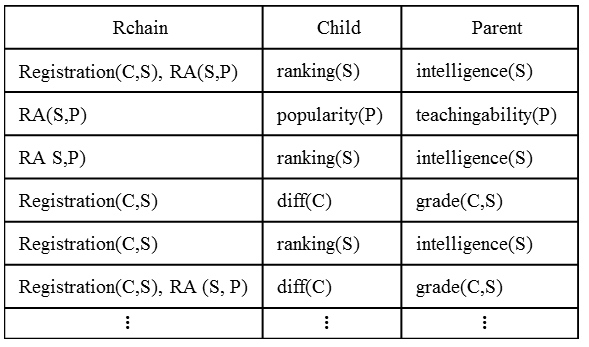
\includegraphics[width=0.3\textwidth]{figures/path-bn.png}
%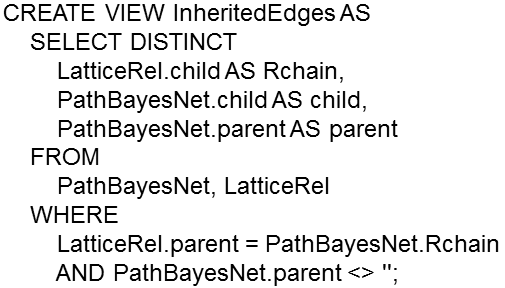
\includegraphics[width=0.3\textwidth]{figures/inherited-view.png}
%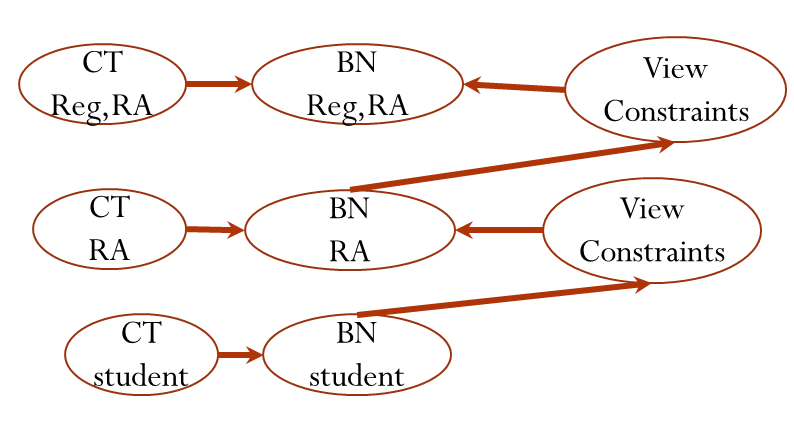
\includegraphics[width=0.3\textwidth]{figures/view-flow.png}
%}
%\caption{Path bayes net and Edge Propagation
%\label{fig:path-bn}}
%\end{center}
%\end{figure}
%
%\subsection{The Model Manager: Edge Propagation} 
%%\paragraph{The Model Manager: Implementing Hierarchical Model Search in SQL}
%Figure~\ref{figure:flow} illustrates the system flow on part of the relationship lattice. The Bayes net learner receives a CT-table and edge constraints as input, and returns a Bayes net. The view mechanism propagates the results as constraints of learning to larger relationship chains, without the need for any further computation.
%
%The Bayes multinet can be stored in a master table called {\em PathBayesNet}, as shown in Figure \ref{fig:path-bn}. An entry such as $$\langle [\it{Registered}(\S,\C),\it{RA}(\S,\P)],\it{ranking}(\S),\it{intelligence}(\S)\rangle$$ means that the 
%Bayes net graph for the relationship chain $\it{Registered}(\S,\C),\it{RA}(\S,\P)$ contains an edge $\it{ranking}(\S)\leftarrow \it{intelligence}(\S)$. 

%
%\begin{figure}[htbp]
%\begin{center}
%\resizebox{0.5\textwidth}{!}{
%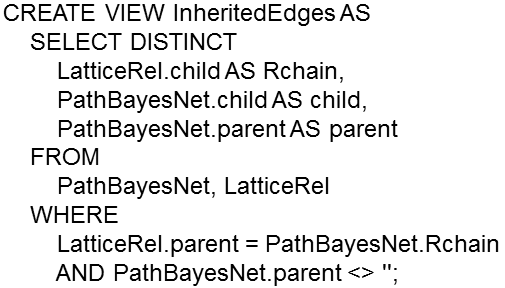
\includegraphics[width=0.3\textwidth]{figures/inherited-view.png}
%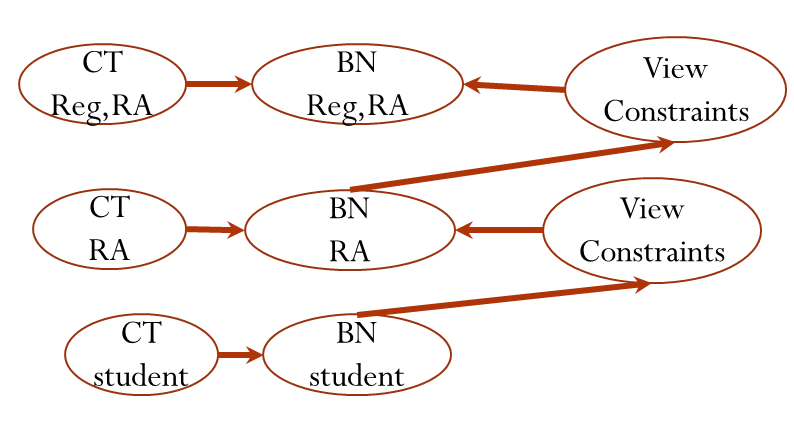
\includegraphics[width=0.3\textwidth]{figures/view-flow.png}
%}
%\caption{Edge Propagation.
%\label{figure:flow}}
%\end{center}
%\end{figure}


%
%The SQL View mechanism propagates edges compactly, as shown in Figure~\ref{fig:path-bn}. 
%%The advantage of the view mechanism is that each time that the Bayes net learner completes learning for a lattice point, the view  update mechanism propagates the results as constraints on learning for the children of the lattice point. 
%The {\em LatticeRel} table records which relationship chains are parents of which others. This auxilliary table makes it easy to write a query that finds, for a given child chain, all the parent chains and inserts their edges as entries for the child chain. This view implements the propagation of required edges. The view definition for forbidden edges is similar: the only difference is that we first need to find the set of complement edges that are {\em not} included in the Bayes net of a given relationship chain. The complement edges are also computed by a view (not shown). 
%




